\documentclass[10pt]{article}
\usepackage[margin=2.2cm]{geometry}
\usepackage{booktabs,longtable,graphicx,array}
\usepackage[hidelinks]{hyperref}
\setlength{\tabcolsep}{4pt}
\newcommand{\stackcell}[1]{\begin{tabular}[t]{@{}l@{}}#1\end{tabular}}
\title{tropical: SubsetSumDecision}
\date{2026-10-25T03:52:34}
\begin{document}
\maketitle

\section{Key results}
This report covers 240 runs (5 seeds; 0 diverged) under frozen hash \texttt{037f987733ac}.
\paragraph{Where to look.} The headline metric is \texttt{ood\_len\_f1} (higher is better).
\autoref{fig:ood_len_f1} plots it against \texttt{fishr\_lambda}.
\autoref{tab:summary-ood_len_f1} gives every cell's mean with its 95\% bootstrap CI.
\autoref{tab:control-ood_len_f1} compares each level with the control.
\autoref{tab:trend-ood_len_f1} gives the trend.
\autoref{tab:paired-ood_len_f1} gives the paired contrasts.
Its tests take the parametric path: values away from the metric bounds.
Cells are compared within a seed: a seed index fixes the data and the initialization.
Comparisons are marked significant at $p < 0.05$ after the stated correction.

\subsection{\texttt{ood\_len\_f1}}
\begin{figure}[tbp]
\centering
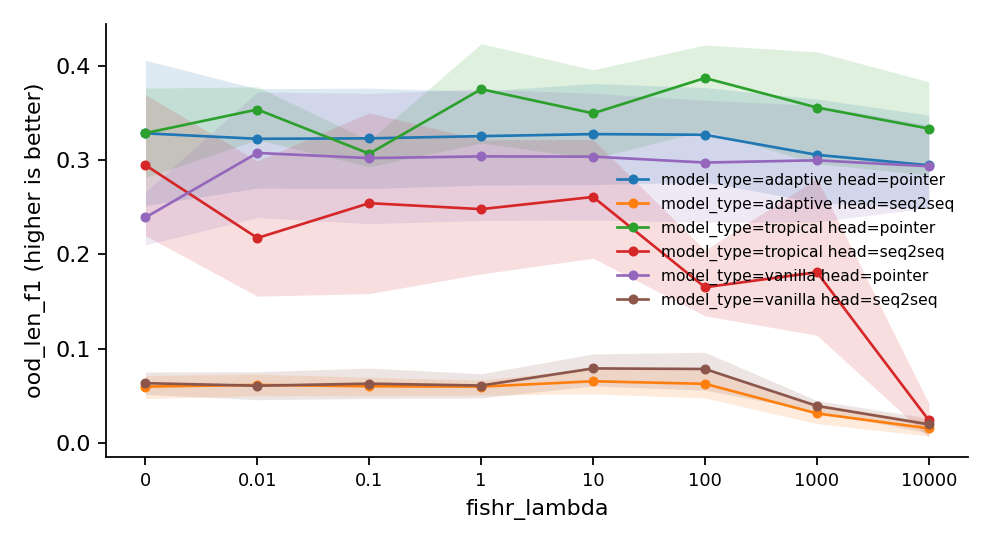
\includegraphics[width=\textwidth]{metric_ood_len_f1.png}
\caption{\texttt{ood\_len\_f1} against \texttt{fishr\_lambda}: the mean over seeds with a 95\% bootstrap CI, one line per combination of the other factors.}
\label{fig:ood_len_f1}
\end{figure}

{\small
\begin{longtable}{lllrlrrr}
\caption{\texttt{ood\_len\_f1} per cell: mean, 95\% bootstrap CI, SD, seeds, diverged runs.}\label{tab:summary-ood_len_f1}\\
\toprule
\texttt{model\_type} & \texttt{head} & \texttt{fishr\_lambda} & mean & 95\% CI & SD & $n$ & div.\\
\midrule
\endhead
adaptive & pointer & 0 & 0.3282 & [0.252, 0.406] & 0.0968 & 5 & 0\\
adaptive & pointer & 0.01 & 0.3224 & [0.27, 0.375] & 0.0726 & 5 & 0\\
adaptive & pointer & 0.1 & 0.3229 & [0.27, 0.376] & 0.0724 & 5 & 0\\
adaptive & pointer & 1 & 0.3252 & [0.273, 0.373] & 0.062 & 5 & 0\\
adaptive & pointer & 10 & 0.3274 & [0.274, 0.381] & 0.0699 & 5 & 0\\
adaptive & pointer & 100 & 0.3267 & [0.277, 0.377] & 0.0666 & 5 & 0\\
adaptive & pointer & 1000 & 0.3054 & [0.255, 0.365] & 0.0724 & 5 & 0\\
adaptive & pointer & 1e+04 & 0.2944 & [0.248, 0.347] & 0.0653 & 5 & 0\\
adaptive & seq2seq & 0 & 0.05996 & [0.0473, 0.0717] & 0.0152 & 5 & 0\\
adaptive & seq2seq & 0.01 & 0.06171 & [0.0502, 0.0732] & 0.0143 & 5 & 0\\
adaptive & seq2seq & 0.1 & 0.0603 & [0.0502, 0.0699] & 0.0126 & 5 & 0\\
adaptive & seq2seq & 1 & 0.05993 & [0.0509, 0.0669] & 0.0108 & 5 & 0\\
adaptive & seq2seq & 10 & 0.06558 & [0.0522, 0.0789] & 0.0177 & 5 & 0\\
adaptive & seq2seq & 100 & 0.06288 & [0.0479, 0.0771] & 0.0193 & 5 & 0\\
adaptive & seq2seq & 1000 & 0.03155 & [0.0207, 0.0418] & 0.0141 & 5 & 0\\
adaptive & seq2seq & 1e+04 & 0.01568 & [0.00754, 0.0228] & 0.0103 & 5 & 0\\
tropical & pointer & 0 & 0.3284 & [0.281, 0.376] & 0.0589 & 5 & 0\\
tropical & pointer & 0.01 & 0.3535 & [0.321, 0.377] & 0.0371 & 5 & 0\\
tropical & pointer & 0.1 & 0.3067 & [0.293, 0.321] & 0.0181 & 5 & 0\\
tropical & pointer & 1 & 0.375 & [0.318, 0.423] & 0.0682 & 5 & 0\\
tropical & pointer & 10 & 0.3494 & [0.301, 0.396] & 0.0651 & 5 & 0\\
tropical & pointer & 100 & 0.3868 & [0.331, 0.422] & 0.0623 & 5 & 0\\
tropical & pointer & 1000 & 0.3556 & [0.296, 0.415] & 0.0768 & 5 & 0\\
tropical & pointer & 1e+04 & 0.3333 & [0.284, 0.383] & 0.0639 & 5 & 0\\
tropical & seq2seq & 0 & 0.2945 & [0.22, 0.369] & 0.0939 & 5 & 0\\
tropical & seq2seq & 0.01 & 0.2174 & [0.156, 0.299] & 0.0967 & 5 & 0\\
tropical & seq2seq & 0.1 & 0.2543 & [0.158, 0.35] & 0.121 & 5 & 0\\
tropical & seq2seq & 1 & 0.2479 & [0.179, 0.321] & 0.092 & 5 & 0\\
tropical & seq2seq & 10 & 0.2608 & [0.196, 0.322] & 0.0859 & 5 & 0\\
tropical & seq2seq & 100 & 0.1651 & [0.135, 0.204] & 0.0469 & 5 & 0\\
tropical & seq2seq & 1000 & 0.1811 & [0.114, 0.28] & 0.112 & 5 & 0\\
tropical & seq2seq & 1e+04 & 0.02423 & [0.00629, 0.0422] & 0.0234 & 5 & 0\\
vanilla & pointer & 0 & 0.2391 & [0.21, 0.266] & 0.0364 & 5 & 0\\
vanilla & pointer & 0.01 & 0.3074 & [0.239, 0.372] & 0.0863 & 5 & 0\\
vanilla & pointer & 0.1 & 0.302 & [0.233, 0.37] & 0.087 & 5 & 0\\
vanilla & pointer & 1 & 0.3038 & [0.236, 0.375] & 0.0896 & 5 & 0\\
vanilla & pointer & 10 & 0.3035 & [0.237, 0.371] & 0.0844 & 5 & 0\\
vanilla & pointer & 100 & 0.2973 & [0.234, 0.363] & 0.0836 & 5 & 0\\
vanilla & pointer & 1000 & 0.2996 & [0.234, 0.358] & 0.0842 & 5 & 0\\
vanilla & pointer & 1e+04 & 0.2933 & [0.249, 0.337] & 0.0602 & 5 & 0\\
vanilla & seq2seq & 0 & 0.06356 & [0.0517, 0.0754] & 0.0151 & 5 & 0\\
vanilla & seq2seq & 0.01 & 0.06088 & [0.0461, 0.0757] & 0.0187 & 5 & 0\\
vanilla & seq2seq & 0.1 & 0.06306 & [0.0473, 0.0796] & 0.0212 & 5 & 0\\
vanilla & seq2seq & 1 & 0.06108 & [0.048, 0.0736] & 0.0166 & 5 & 0\\
vanilla & seq2seq & 10 & 0.07919 & [0.0607, 0.0945] & 0.0229 & 5 & 0\\
vanilla & seq2seq & 100 & 0.07859 & [0.0562, 0.0963] & 0.0264 & 5 & 0\\
vanilla & seq2seq & 1000 & 0.03947 & [0.0338, 0.0452] & 0.00741 & 5 & 0\\
vanilla & seq2seq & 1e+04 & 0.01994 & [0.0107, 0.0266] & 0.0107 & 5 & 0\\
\bottomrule
\end{longtable}
}

{\small
\begin{longtable}{lllrrrl}
\caption{\texttt{ood\_len\_f1}: each level of \texttt{fishr\_lambda} against its control (0), within each combination of the other factors. parametric: Dunnett vs control.}\label{tab:control-ood_len_f1}\\
\toprule
\texttt{model\_type} & \texttt{head} & \texttt{fishr\_lambda} & difference & 95\% CI & $p$ & \\
\midrule
\endhead
adaptive & pointer & 0.01 & -0.005812 & [-0.133, 0.122] & 1.0000 & \\
adaptive & pointer & 0.1 & -0.005338 & [-0.133, 0.122] & 1.0000 & \\
adaptive & pointer & 1 & -0.003003 & [-0.13, 0.124] & 1.0000 & \\
adaptive & pointer & 10 & $-8.349\times10^{-4}$ & [-0.128, 0.127] & 1.0000 & \\
adaptive & pointer & 100 & -0.001539 & [-0.129, 0.126] & 1.0000 & \\
adaptive & pointer & 1000 & -0.0228 & [-0.15, 0.105] & 0.9957 & \\
adaptive & pointer & 1e+04 & -0.03384 & [-0.161, 0.0936] & 0.9625 & \\
adaptive & seq2seq & 0.01 & 0.00175 & [-0.0237, 0.0272] & 1.0000 & \\
adaptive & seq2seq & 0.1 & $3.382\times10^{-4}$ & [-0.0251, 0.0258] & 1.0000 & \\
adaptive & seq2seq & 1 & $-2.794\times10^{-5}$ & [-0.0255, 0.0254] & 1.0000 & \\
adaptive & seq2seq & 10 & 0.00562 & [-0.0199, 0.0311] & 0.9857 & \\
adaptive & seq2seq & 100 & 0.002922 & [-0.0226, 0.0284] & 0.9997 & \\
adaptive & seq2seq & 1000 & -0.02841 & [-0.0539, -0.00293] & 0.0236 & *\\
adaptive & seq2seq & 1e+04 & -0.04428 & [-0.0698, -0.0188] & 0.0002 & *\\
tropical & pointer & 0.01 & 0.02501 & [-0.0782, 0.128] & 0.9764 & \\
tropical & pointer & 0.1 & -0.02179 & [-0.125, 0.0814] & 0.9888 & \\
tropical & pointer & 1 & 0.04655 & [-0.0566, 0.15] & 0.6969 & \\
tropical & pointer & 10 & 0.02096 & [-0.0822, 0.124] & 0.9910 & \\
tropical & pointer & 100 & 0.05835 & [-0.0449, 0.162] & 0.4768 & \\
tropical & pointer & 1000 & 0.02712 & [-0.0761, 0.13] & 0.9644 & \\
tropical & pointer & 1e+04 & 0.00482 & [-0.0984, 0.108] & 1.0000 & \\
tropical & seq2seq & 0.01 & -0.07714 & [-0.233, 0.0791] & 0.6135 & \\
tropical & seq2seq & 0.1 & -0.04025 & [-0.196, 0.116] & 0.9678 & \\
tropical & seq2seq & 1 & -0.04659 & [-0.203, 0.11] & 0.9352 & \\
tropical & seq2seq & 10 & -0.03367 & [-0.19, 0.123] & 0.9874 & \\
tropical & seq2seq & 100 & -0.1294 & [-0.286, 0.0269] & 0.1382 & \\
tropical & seq2seq & 1000 & -0.1134 & [-0.27, 0.0428] & 0.2353 & \\
tropical & seq2seq & 1e+04 & -0.2703 & [-0.427, -0.114] & 0.0002 & *\\
vanilla & pointer & 0.01 & 0.06833 & [-0.0687, 0.205] & 0.6035 & \\
vanilla & pointer & 0.1 & 0.06287 & [-0.0741, 0.2] & 0.6818 & \\
vanilla & pointer & 1 & 0.06468 & [-0.0723, 0.202] & 0.6558 & \\
vanilla & pointer & 10 & 0.06443 & [-0.0726, 0.201] & 0.6593 & \\
vanilla & pointer & 100 & 0.05816 & [-0.0788, 0.195] & 0.7473 & \\
vanilla & pointer & 1000 & 0.06054 & [-0.0765, 0.198] & 0.7146 & \\
vanilla & pointer & 1e+04 & 0.05421 & [-0.0828, 0.191] & 0.7995 & \\
vanilla & seq2seq & 0.01 & -0.002683 & [-0.0348, 0.0294] & 1.0000 & \\
vanilla & seq2seq & 0.1 & $-5.058\times10^{-4}$ & [-0.0326, 0.0316] & 1.0000 & \\
vanilla & seq2seq & 1 & -0.002484 & [-0.0346, 0.0296] & 1.0000 & \\
vanilla & seq2seq & 10 & 0.01563 & [-0.0164, 0.0477] & 0.6259 & \\
vanilla & seq2seq & 100 & 0.01502 & [-0.017, 0.0471] & 0.6629 & \\
vanilla & seq2seq & 1000 & -0.02409 & [-0.0562, 0.00797] & 0.2072 & \\
vanilla & seq2seq & 1e+04 & -0.04363 & [-0.0757, -0.0116] & 0.0042 & *\\
\bottomrule
\end{longtable}
}

{\small
\begin{longtable}{llrrrrr}
\caption{\texttt{ood\_len\_f1} against log10 \texttt{fishr\_lambda}: parametric: OLS slope t-test, seed-bootstrap CI, with the Jonckheere--Terpstra ordered-trend $\tau$ and $p$.}\label{tab:trend-ood_len_f1}\\
\toprule
\texttt{model\_type} & \texttt{head} & estimate & 95\% CI & $p$ & JT $\tau$ & JT $p$\\
\midrule
\endhead
adaptive & pointer & -0.004198 & [-0.0112, 0.00103] & 0.4432 & -0.116 & 0.3915\\
adaptive & seq2seq & -0.00688 & [-0.00807, -0.00571] & $<10^{-4}$ & -0.455 & 0.0004\\
tropical & pointer & 0.001751 & [-0.00287, 0.00605] & 0.7314 & 0.0286 & 0.8382\\
tropical & seq2seq & -0.02888 & [-0.0474, -0.0158] & 0.0013 & -0.429 & 0.0012\\
vanilla & pointer & -0.001912 & [-0.0084, 0.00314] & 0.7684 & -0.0743 & 0.5889\\
vanilla & seq2seq & -0.005446 & [-0.00743, -0.00301] & 0.0117 & -0.326 & 0.0136\\
\bottomrule
\end{longtable}
}

{\small
\begin{longtable}{lrrrl}
\caption{\texttt{ood\_len\_f1}: paired contrasts by seed, Holm-corrected across the cells. parametric: paired t-test by seed, Holm.}\label{tab:paired-ood_len_f1}\\
\toprule
contrast (within) & difference & 95\% CI & $p$ & \\
\midrule
\endhead
\stackcell{model\_type: tropical - vanilla\\\footnotesize head=pointer fishr\_lambda=0 } & 0.08934 & [0.00597, 0.173] & 0.4093 & \\
\stackcell{model\_type: tropical - vanilla\\\footnotesize head=pointer fishr\_lambda=0.01 } & 0.04602 & [-0.0763, 0.168] & 1.0000 & \\
\stackcell{model\_type: tropical - vanilla\\\footnotesize head=pointer fishr\_lambda=0.1 } & 0.004687 & [-0.122, 0.131] & 1.0000 & \\
\stackcell{model\_type: tropical - vanilla\\\footnotesize head=pointer fishr\_lambda=1 } & 0.07121 & [-0.0835, 0.226] & 1.0000 & \\
\stackcell{model\_type: tropical - vanilla\\\footnotesize head=pointer fishr\_lambda=10 } & 0.04587 & [-0.124, 0.215] & 1.0000 & \\
\stackcell{model\_type: tropical - vanilla\\\footnotesize head=pointer fishr\_lambda=100 } & 0.08953 & [-0.0535, 0.233] & 1.0000 & \\
\stackcell{model\_type: tropical - vanilla\\\footnotesize head=pointer fishr\_lambda=1000 } & 0.05592 & [-0.121, 0.233] & 1.0000 & \\
\stackcell{model\_type: tropical - vanilla\\\footnotesize head=pointer fishr\_lambda=1e+04 } & 0.03995 & [-0.064, 0.144] & 1.0000 & \\
\stackcell{model\_type: tropical - vanilla\\\footnotesize head=seq2seq fishr\_lambda=0 } & 0.2309 & [0.132, 0.33] & 0.0463 & *\\
\stackcell{model\_type: tropical - vanilla\\\footnotesize head=seq2seq fishr\_lambda=0.01 } & 0.1565 & [0.0256, 0.287] & 0.3466 & \\
\stackcell{model\_type: tropical - vanilla\\\footnotesize head=seq2seq fishr\_lambda=0.1 } & 0.1912 & [0.0322, 0.35] & 0.3466 & \\
\stackcell{model\_type: tropical - vanilla\\\footnotesize head=seq2seq fishr\_lambda=1 } & 0.1868 & [0.0697, 0.304] & 0.1714 & \\
\stackcell{model\_type: tropical - vanilla\\\footnotesize head=seq2seq fishr\_lambda=10 } & 0.1816 & [0.0677, 0.296] & 0.1714 & \\
\stackcell{model\_type: tropical - vanilla\\\footnotesize head=seq2seq fishr\_lambda=100 } & 0.08655 & [0.0296, 0.144] & 0.1753 & \\
\stackcell{model\_type: tropical - vanilla\\\footnotesize head=seq2seq fishr\_lambda=1000 } & 0.1416 & [$7.96\times10^{-5}$, 0.283] & 0.4493 & \\
\stackcell{model\_type: tropical - vanilla\\\footnotesize head=seq2seq fishr\_lambda=1e+04 } & 0.004291 & [-0.0189, 0.0275] & 1.0000 & \\
\stackcell{model\_type: adaptive - vanilla\\\footnotesize head=pointer fishr\_lambda=0 } & 0.08913 & [-0.0738, 0.252] & 1.0000 & \\
\stackcell{model\_type: adaptive - vanilla\\\footnotesize head=pointer fishr\_lambda=0.01 } & 0.01498 & [-0.0695, 0.0995] & 1.0000 & \\
\stackcell{model\_type: adaptive - vanilla\\\footnotesize head=pointer fishr\_lambda=0.1 } & 0.02092 & [-0.0638, 0.106] & 1.0000 & \\
\stackcell{model\_type: adaptive - vanilla\\\footnotesize head=pointer fishr\_lambda=1 } & 0.02144 & [-0.0708, 0.114] & 1.0000 & \\
\stackcell{model\_type: adaptive - vanilla\\\footnotesize head=pointer fishr\_lambda=10 } & 0.02386 & [-0.0718, 0.12] & 1.0000 & \\
\stackcell{model\_type: adaptive - vanilla\\\footnotesize head=pointer fishr\_lambda=100 } & 0.02943 & [-0.0681, 0.127] & 1.0000 & \\
\stackcell{model\_type: adaptive - vanilla\\\footnotesize head=pointer fishr\_lambda=1000 } & 0.005788 & [-0.0753, 0.0869] & 1.0000 & \\
\stackcell{model\_type: adaptive - vanilla\\\footnotesize head=pointer fishr\_lambda=1e+04 } & 0.001073 & [-0.0905, 0.0926] & 1.0000 & \\
\stackcell{model\_type: adaptive - vanilla\\\footnotesize head=seq2seq fishr\_lambda=0 } & -0.003601 & [-0.012, 0.00479] & 1.0000 & \\
\stackcell{model\_type: adaptive - vanilla\\\footnotesize head=seq2seq fishr\_lambda=0.01 } & $8.320\times10^{-4}$ & [-0.0114, 0.013] & 1.0000 & \\
\stackcell{model\_type: adaptive - vanilla\\\footnotesize head=seq2seq fishr\_lambda=0.1 } & -0.002757 & [-0.019, 0.0135] & 1.0000 & \\
\stackcell{model\_type: adaptive - vanilla\\\footnotesize head=seq2seq fishr\_lambda=1 } & -0.001145 & [-0.0122, 0.0099] & 1.0000 & \\
\stackcell{model\_type: adaptive - vanilla\\\footnotesize head=seq2seq fishr\_lambda=10 } & -0.01361 & [-0.0432, 0.016] & 1.0000 & \\
\stackcell{model\_type: adaptive - vanilla\\\footnotesize head=seq2seq fishr\_lambda=100 } & -0.0157 & [-0.0363, 0.0049] & 1.0000 & \\
\stackcell{model\_type: adaptive - vanilla\\\footnotesize head=seq2seq fishr\_lambda=1000 } & -0.007917 & [-0.0209, 0.00511] & 1.0000 & \\
\stackcell{model\_type: adaptive - vanilla\\\footnotesize head=seq2seq fishr\_lambda=1e+04 } & -0.004252 & [-0.0129, 0.00439] & 1.0000 & \\
\stackcell{head: pointer - seq2seq\\\footnotesize model\_type=adaptive fishr\_lambda=0 } & 0.2683 & [0.159, 0.378] & 0.0335 & *\\
\stackcell{head: pointer - seq2seq\\\footnotesize model\_type=adaptive fishr\_lambda=0.01 } & 0.2607 & [0.159, 0.363] & 0.0335 & *\\
\stackcell{head: pointer - seq2seq\\\footnotesize model\_type=adaptive fishr\_lambda=0.1 } & 0.2626 & [0.162, 0.363] & 0.0329 & *\\
\stackcell{head: pointer - seq2seq\\\footnotesize model\_type=adaptive fishr\_lambda=1 } & 0.2653 & [0.179, 0.351] & 0.0204 & *\\
\stackcell{head: pointer - seq2seq\\\footnotesize model\_type=adaptive fishr\_lambda=10 } & 0.2618 & [0.158, 0.365] & 0.0335 & *\\
\stackcell{head: pointer - seq2seq\\\footnotesize model\_type=adaptive fishr\_lambda=100 } & 0.2638 & [0.167, 0.361] & 0.0295 & *\\
\stackcell{head: pointer - seq2seq\\\footnotesize model\_type=adaptive fishr\_lambda=1000 } & 0.2739 & [0.182, 0.365] & 0.0218 & *\\
\stackcell{head: pointer - seq2seq\\\footnotesize model\_type=adaptive fishr\_lambda=1e+04 } & 0.2787 & [0.203, 0.354] & 0.0123 & *\\
\stackcell{head: pointer - seq2seq\\\footnotesize model\_type=tropical fishr\_lambda=0 } & 0.03394 & [-0.145, 0.213] & 0.7623 & \\
\stackcell{head: pointer - seq2seq\\\footnotesize model\_type=tropical fishr\_lambda=0.01 } & 0.1361 & [0.0247, 0.247] & 0.1647 & \\
\stackcell{head: pointer - seq2seq\\\footnotesize model\_type=tropical fishr\_lambda=0.1 } & 0.0524 & [-0.0956, 0.2] & 0.7623 & \\
\stackcell{head: pointer - seq2seq\\\footnotesize model\_type=tropical fishr\_lambda=1 } & 0.1271 & [-0.0312, 0.285] & 0.2691 & \\
\stackcell{head: pointer - seq2seq\\\footnotesize model\_type=tropical fishr\_lambda=10 } & 0.08857 & [0.0035, 0.174] & 0.1781 & \\
\stackcell{head: pointer - seq2seq\\\footnotesize model\_type=tropical fishr\_lambda=100 } & 0.2217 & [0.0919, 0.351] & 0.0631 & \\
\stackcell{head: pointer - seq2seq\\\footnotesize model\_type=tropical fishr\_lambda=1000 } & 0.1745 & [0.0252, 0.324] & 0.1647 & \\
\stackcell{head: pointer - seq2seq\\\footnotesize model\_type=tropical fishr\_lambda=1e+04 } & 0.309 & [0.221, 0.397] & 0.0134 & *\\
\stackcell{head: pointer - seq2seq\\\footnotesize model\_type=vanilla fishr\_lambda=0 } & 0.1755 & [0.121, 0.23] & 0.0183 & *\\
\stackcell{head: pointer - seq2seq\\\footnotesize model\_type=vanilla fishr\_lambda=0.01 } & 0.2466 & [0.132, 0.361] & 0.0396 & *\\
\stackcell{head: pointer - seq2seq\\\footnotesize model\_type=vanilla fishr\_lambda=0.1 } & 0.2389 & [0.124, 0.354] & 0.0408 & *\\
\stackcell{head: pointer - seq2seq\\\footnotesize model\_type=vanilla fishr\_lambda=1 } & 0.2427 & [0.125, 0.36] & 0.0408 & *\\
\stackcell{head: pointer - seq2seq\\\footnotesize model\_type=vanilla fishr\_lambda=10 } & 0.2243 & [0.134, 0.315] & 0.0335 & *\\
\stackcell{head: pointer - seq2seq\\\footnotesize model\_type=vanilla fishr\_lambda=100 } & 0.2187 & [0.13, 0.307] & 0.0335 & *\\
\stackcell{head: pointer - seq2seq\\\footnotesize model\_type=vanilla fishr\_lambda=1000 } & 0.2602 & [0.156, 0.364] & 0.0335 & *\\
\stackcell{head: pointer - seq2seq\\\footnotesize model\_type=vanilla fishr\_lambda=1e+04 } & 0.2734 & [0.198, 0.349] & 0.0125 & *\\
\bottomrule
\end{longtable}
}

\clearpage
\appendix
\section{Other metrics}
\subsection{\texttt{ood\_len\_exact}}
\begin{figure}[tbp]
\centering
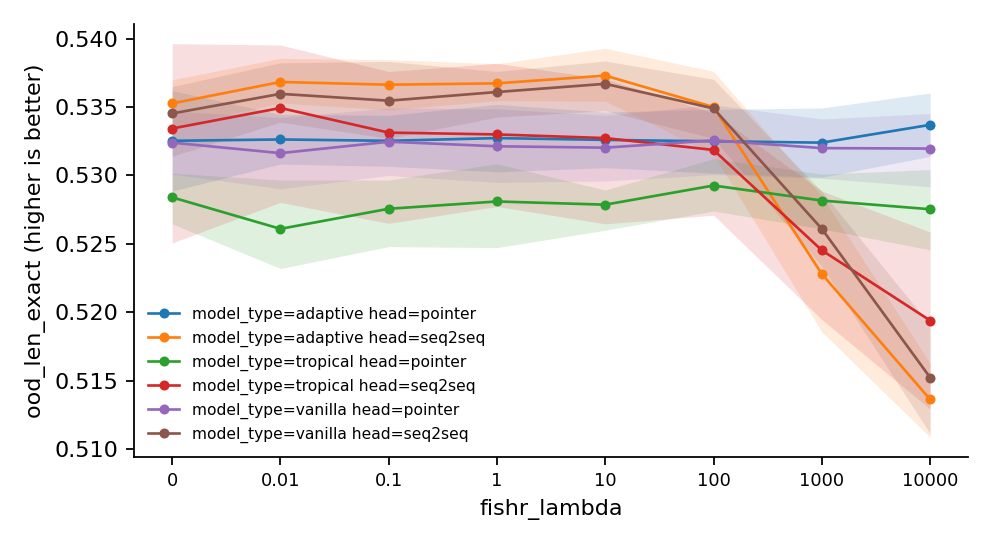
\includegraphics[width=\textwidth]{metric_ood_len_exact.png}
\caption{\texttt{ood\_len\_exact} against \texttt{fishr\_lambda}: the mean over seeds with a 95\% bootstrap CI, one line per combination of the other factors.}
\label{fig:ood_len_exact}
\end{figure}

{\small
\begin{longtable}{lllrlrrr}
\caption{\texttt{ood\_len\_exact} per cell: mean, 95\% bootstrap CI, SD, seeds, diverged runs.}\label{tab:summary-ood_len_exact}\\
\toprule
\texttt{model\_type} & \texttt{head} & \texttt{fishr\_lambda} & mean & 95\% CI & SD & $n$ & div.\\
\midrule
\endhead
adaptive & pointer & 0 & 0.5325 & [0.529, 0.536] & 0.0048 & 5 & 0\\
adaptive & pointer & 0.01 & 0.5326 & [0.531, 0.534] & 0.0024 & 5 & 0\\
adaptive & pointer & 0.1 & 0.5325 & [0.531, 0.534] & 0.00249 & 5 & 0\\
adaptive & pointer & 1 & 0.5327 & [0.53, 0.535] & 0.0032 & 5 & 0\\
adaptive & pointer & 10 & 0.5326 & [0.531, 0.535] & 0.00259 & 5 & 0\\
adaptive & pointer & 100 & 0.5325 & [0.53, 0.535] & 0.00297 & 5 & 0\\
adaptive & pointer & 1000 & 0.5324 & [0.53, 0.535] & 0.00344 & 5 & 0\\
adaptive & pointer & 1e+04 & 0.5337 & [0.531, 0.536] & 0.003 & 5 & 0\\
adaptive & seq2seq & 0 & 0.5353 & [0.534, 0.537] & 0.00219 & 5 & 0\\
adaptive & seq2seq & 0.01 & 0.5368 & [0.535, 0.539] & 0.0021 & 5 & 0\\
adaptive & seq2seq & 0.1 & 0.5366 & [0.535, 0.538] & 0.00255 & 5 & 0\\
adaptive & seq2seq & 1 & 0.5367 & [0.535, 0.538] & 0.00171 & 5 & 0\\
adaptive & seq2seq & 10 & 0.5373 & [0.535, 0.539] & 0.00247 & 5 & 0\\
adaptive & seq2seq & 100 & 0.535 & [0.532, 0.538] & 0.00414 & 5 & 0\\
adaptive & seq2seq & 1000 & 0.5228 & [0.519, 0.528] & 0.00641 & 5 & 0\\
adaptive & seq2seq & 1e+04 & 0.5136 & [0.511, 0.516] & 0.00366 & 5 & 0\\
tropical & pointer & 0 & 0.5284 & [0.526, 0.53] & 0.0025 & 5 & 0\\
tropical & pointer & 0.01 & 0.5261 & [0.523, 0.53] & 0.00403 & 5 & 0\\
tropical & pointer & 0.1 & 0.5276 & [0.525, 0.53] & 0.00307 & 5 & 0\\
tropical & pointer & 1 & 0.5281 & [0.525, 0.531] & 0.00398 & 5 & 0\\
tropical & pointer & 10 & 0.5279 & [0.526, 0.529] & 0.00208 & 5 & 0\\
tropical & pointer & 100 & 0.5293 & [0.527, 0.531] & 0.00241 & 5 & 0\\
tropical & pointer & 1000 & 0.5282 & [0.526, 0.53] & 0.00258 & 5 & 0\\
tropical & pointer & 1e+04 & 0.5275 & [0.525, 0.53] & 0.00382 & 5 & 0\\
tropical & seq2seq & 0 & 0.5334 & [0.525, 0.54] & 0.00914 & 5 & 0\\
tropical & seq2seq & 0.01 & 0.5349 & [0.528, 0.54] & 0.00779 & 5 & 0\\
tropical & seq2seq & 0.1 & 0.5331 & [0.527, 0.538] & 0.0075 & 5 & 0\\
tropical & seq2seq & 1 & 0.533 & [0.528, 0.538] & 0.0064 & 5 & 0\\
tropical & seq2seq & 10 & 0.5327 & [0.526, 0.537] & 0.00751 & 5 & 0\\
tropical & seq2seq & 100 & 0.5319 & [0.527, 0.535] & 0.00526 & 5 & 0\\
tropical & seq2seq & 1000 & 0.5245 & [0.519, 0.529] & 0.00604 & 5 & 0\\
tropical & seq2seq & 1e+04 & 0.5194 & [0.513, 0.526] & 0.00881 & 5 & 0\\
vanilla & pointer & 0 & 0.5324 & [0.53, 0.535] & 0.00299 & 5 & 0\\
vanilla & pointer & 0.01 & 0.5316 & [0.529, 0.534] & 0.00331 & 5 & 0\\
vanilla & pointer & 0.1 & 0.5325 & [0.53, 0.535] & 0.00313 & 5 & 0\\
vanilla & pointer & 1 & 0.5321 & [0.529, 0.535] & 0.00349 & 5 & 0\\
vanilla & pointer & 10 & 0.532 & [0.53, 0.534] & 0.00305 & 5 & 0\\
vanilla & pointer & 100 & 0.5326 & [0.53, 0.535] & 0.00335 & 5 & 0\\
vanilla & pointer & 1000 & 0.532 & [0.53, 0.534] & 0.00271 & 5 & 0\\
vanilla & pointer & 1e+04 & 0.532 & [0.529, 0.535] & 0.00344 & 5 & 0\\
vanilla & seq2seq & 0 & 0.5345 & [0.531, 0.536] & 0.00354 & 5 & 0\\
vanilla & seq2seq & 0.01 & 0.536 & [0.534, 0.538] & 0.00261 & 5 & 0\\
vanilla & seq2seq & 0.1 & 0.5355 & [0.533, 0.538] & 0.0036 & 5 & 0\\
vanilla & seq2seq & 1 & 0.5361 & [0.534, 0.538] & 0.00214 & 5 & 0\\
vanilla & seq2seq & 10 & 0.5367 & [0.535, 0.538] & 0.00222 & 5 & 0\\
vanilla & seq2seq & 100 & 0.5349 & [0.533, 0.537] & 0.00285 & 5 & 0\\
vanilla & seq2seq & 1000 & 0.5261 & [0.523, 0.529] & 0.00365 & 5 & 0\\
vanilla & seq2seq & 1e+04 & 0.5152 & [0.511, 0.519] & 0.00529 & 5 & 0\\
\bottomrule
\end{longtable}
}

{\small
\begin{longtable}{lllrrrl}
\caption{\texttt{ood\_len\_exact}: each level of \texttt{fishr\_lambda} against its control (0), within each combination of the other factors. parametric: Dunnett vs control.}\label{tab:control-ood_len_exact}\\
\toprule
\texttt{model\_type} & \texttt{head} & \texttt{fishr\_lambda} & difference & 95\% CI & $p$ & \\
\midrule
\endhead
adaptive & pointer & 0.01 & $1.000\times10^{-4}$ & [-0.00548, 0.00568] & 1.0000 & \\
adaptive & pointer & 0.1 & $-1.110\times10^{-16}$ & [-0.00558, 0.00558] & 1.0000 & \\
adaptive & pointer & 1 & $2.000\times10^{-4}$ & [-0.00538, 0.00578] & 1.0000 & \\
adaptive & pointer & 10 & $6.667\times10^{-5}$ & [-0.00551, 0.00565] & 1.0000 & \\
adaptive & pointer & 100 & $-3.333\times10^{-5}$ & [-0.00561, 0.00555] & 1.0000 & \\
adaptive & pointer & 1000 & $-1.333\times10^{-4}$ & [-0.00571, 0.00545] & 1.0000 & \\
adaptive & pointer & 1e+04 & 0.001167 & [-0.00441, 0.00675] & 0.9894 & \\
adaptive & seq2seq & 0.01 & 0.001567 & [-0.0045, 0.00763] & 0.9673 & \\
adaptive & seq2seq & 0.1 & 0.001367 & [-0.0047, 0.00743] & 0.9839 & \\
adaptive & seq2seq & 1 & 0.001467 & [-0.0046, 0.00753] & 0.9766 & \\
adaptive & seq2seq & 10 & 0.002033 & [-0.00403, 0.0081] & 0.8923 & \\
adaptive & seq2seq & 100 & $-2.667\times10^{-4}$ & [-0.00633, 0.0058] & 1.0000 & \\
adaptive & seq2seq & 1000 & -0.01247 & [-0.0185, -0.0064] & $<10^{-4}$ & *\\
adaptive & seq2seq & 1e+04 & -0.02163 & [-0.0277, -0.0156] & $<10^{-4}$ & *\\
tropical & pointer & 0.01 & -0.0023 & [-0.00779, 0.00319] & 0.7578 & \\
tropical & pointer & 0.1 & $-8.333\times10^{-4}$ & [-0.00632, 0.00466] & 0.9984 & \\
tropical & pointer & 1 & $-3.000\times10^{-4}$ & [-0.00579, 0.00519] & 1.0000 & \\
tropical & pointer & 10 & $-5.333\times10^{-4}$ & [-0.00602, 0.00496] & 0.9999 & \\
tropical & pointer & 100 & $8.667\times10^{-4}$ & [-0.00462, 0.00636] & 0.9980 & \\
tropical & pointer & 1000 & $-2.333\times10^{-4}$ & [-0.00572, 0.00526] & 1.0000 & \\
tropical & pointer & 1e+04 & $-8.667\times10^{-4}$ & [-0.00636, 0.00462] & 0.9980 & \\
tropical & seq2seq & 0.01 & 0.0015 & [-0.0114, 0.0144] & 0.9997 & \\
tropical & seq2seq & 0.1 & $-3.000\times10^{-4}$ & [-0.0132, 0.0126] & 1.0000 & \\
tropical & seq2seq & 1 & $-4.333\times10^{-4}$ & [-0.0134, 0.0125] & 1.0000 & \\
tropical & seq2seq & 10 & $-7.000\times10^{-4}$ & [-0.0136, 0.0122] & 1.0000 & \\
tropical & seq2seq & 100 & -0.001567 & [-0.0145, 0.0114] & 0.9996 & \\
tropical & seq2seq & 1000 & -0.0089 & [-0.0218, 0.00405] & 0.2833 & \\
tropical & seq2seq & 1e+04 & -0.01403 & [-0.027, -0.00108] & 0.0292 & *\\
vanilla & pointer & 0.01 & $-7.667\times10^{-4}$ & [-0.00635, 0.00481] & 0.9991 & \\
vanilla & pointer & 0.1 & $6.667\times10^{-5}$ & [-0.00551, 0.00565] & 1.0000 & \\
vanilla & pointer & 1 & $-2.667\times10^{-4}$ & [-0.00585, 0.00531] & 1.0000 & \\
vanilla & pointer & 10 & $-3.667\times10^{-4}$ & [-0.00595, 0.00521] & 1.0000 & \\
vanilla & pointer & 100 & $1.667\times10^{-4}$ & [-0.00541, 0.00575] & 1.0000 & \\
vanilla & pointer & 1000 & $-4.000\times10^{-4}$ & [-0.00598, 0.00518] & 1.0000 & \\
vanilla & pointer & 1e+04 & $-4.333\times10^{-4}$ & [-0.00601, 0.00515] & 1.0000 & \\
vanilla & seq2seq & 0.01 & 0.001433 & [-0.00446, 0.00733] & 0.9761 & \\
vanilla & seq2seq & 0.1 & $9.333\times10^{-4}$ & [-0.00496, 0.00683] & 0.9979 & \\
vanilla & seq2seq & 1 & 0.001567 & [-0.00433, 0.00746] & 0.9625 & \\
vanilla & seq2seq & 10 & 0.002167 & [-0.00373, 0.00806] & 0.8463 & \\
vanilla & seq2seq & 100 & $3.667\times10^{-4}$ & [-0.00553, 0.00626] & 1.0000 & \\
vanilla & seq2seq & 1000 & -0.008433 & [-0.0143, -0.00254] & 0.0025 & *\\
vanilla & seq2seq & 1e+04 & -0.0193 & [-0.0252, -0.0134] & $<10^{-4}$ & *\\
\bottomrule
\end{longtable}
}

{\small
\begin{longtable}{llrrrrr}
\caption{\texttt{ood\_len\_exact} against log10 \texttt{fishr\_lambda}: parametric: OLS slope t-test, seed-bootstrap CI, with the Jonckheere--Terpstra ordered-trend $\tau$ and $p$.}\label{tab:trend-ood_len_exact}\\
\toprule
\texttt{model\_type} & \texttt{head} & estimate & 95\% CI & $p$ & JT $\tau$ & JT $p$\\
\midrule
\endhead
adaptive & pointer & $9.643\times10^{-5}$ & [$-7.50\times10^{-5}$, $2.63\times10^{-4}$] & 0.6743 & 0.0724 & 0.6001\\
adaptive & seq2seq & -0.003536 & [-0.00406, -0.00286] & $<10^{-4}$ & -0.52 & 0.0002\\
tropical & pointer & $2.381\times10^{-4}$ & [$-2.26\times10^{-5}$, $4.99\times10^{-4}$] & 0.3649 & 0.105 & 0.4441\\
tropical & seq2seq & -0.002319 & [-0.00357, -0.00107] & 0.0005 & -0.503 & 0.0004\\
vanilla & pointer & $1.786\times10^{-5}$ & [$-8.10\times10^{-5}$, $1.17\times10^{-4}$] & 0.9440 & 0.0552 & 0.6783\\
vanilla & seq2seq & -0.002933 & [-0.00356, -0.00224] & $<10^{-4}$ & -0.497 & 0.0002\\
\bottomrule
\end{longtable}
}

{\small
\begin{longtable}{lrrrl}
\caption{\texttt{ood\_len\_exact}: paired contrasts by seed, Holm-corrected across the cells. parametric: paired t-test by seed, Holm.}\label{tab:paired-ood_len_exact}\\
\toprule
contrast (within) & difference & 95\% CI & $p$ & \\
\midrule
\endhead
\stackcell{model\_type: tropical - vanilla\\\footnotesize head=pointer fishr\_lambda=0 } & -0.004 & [-0.00639, -0.00161] & 0.1358 & \\
\stackcell{model\_type: tropical - vanilla\\\footnotesize head=pointer fishr\_lambda=0.01 } & -0.005533 & [-0.00939, -0.00168] & 0.1987 & \\
\stackcell{model\_type: tropical - vanilla\\\footnotesize head=pointer fishr\_lambda=0.1 } & -0.0049 & [-0.00857, -0.00123] & 0.2087 & \\
\stackcell{model\_type: tropical - vanilla\\\footnotesize head=pointer fishr\_lambda=1 } & -0.004033 & [-0.00679, -0.00128] & 0.1987 & \\
\stackcell{model\_type: tropical - vanilla\\\footnotesize head=pointer fishr\_lambda=10 } & -0.004167 & [-0.0072, -0.00113] & 0.2087 & \\
\stackcell{model\_type: tropical - vanilla\\\footnotesize head=pointer fishr\_lambda=100 } & -0.0033 & [-0.00468, -0.00192] & 0.0432 & *\\
\stackcell{model\_type: tropical - vanilla\\\footnotesize head=pointer fishr\_lambda=1000 } & -0.003833 & [-0.00561, -0.00205] & 0.0590 & \\
\stackcell{model\_type: tropical - vanilla\\\footnotesize head=pointer fishr\_lambda=1e+04 } & -0.004433 & [-0.00851, $-3.53\times10^{-4}$] & 0.3537 & \\
\stackcell{model\_type: tropical - vanilla\\\footnotesize head=seq2seq fishr\_lambda=0 } & -0.0011 & [-0.00896, 0.00676] & 1.0000 & \\
\stackcell{model\_type: tropical - vanilla\\\footnotesize head=seq2seq fishr\_lambda=0.01 } & -0.001033 & [-0.00832, 0.00625] & 1.0000 & \\
\stackcell{model\_type: tropical - vanilla\\\footnotesize head=seq2seq fishr\_lambda=0.1 } & -0.002333 & [-0.00981, 0.00514] & 1.0000 & \\
\stackcell{model\_type: tropical - vanilla\\\footnotesize head=seq2seq fishr\_lambda=1 } & -0.0031 & [-0.00873, 0.00253] & 1.0000 & \\
\stackcell{model\_type: tropical - vanilla\\\footnotesize head=seq2seq fishr\_lambda=10 } & -0.003967 & [-0.0116, 0.00367] & 1.0000 & \\
\stackcell{model\_type: tropical - vanilla\\\footnotesize head=seq2seq fishr\_lambda=100 } & -0.003033 & [-0.00793, 0.00186] & 1.0000 & \\
\stackcell{model\_type: tropical - vanilla\\\footnotesize head=seq2seq fishr\_lambda=1000 } & -0.001567 & [-0.00673, 0.0036] & 1.0000 & \\
\stackcell{model\_type: tropical - vanilla\\\footnotesize head=seq2seq fishr\_lambda=1e+04 } & 0.004167 & [-0.00613, 0.0145] & 1.0000 & \\
\stackcell{model\_type: adaptive - vanilla\\\footnotesize head=pointer fishr\_lambda=0 } & $1.333\times10^{-4}$ & [-0.00318, 0.00345] & 1.0000 & \\
\stackcell{model\_type: adaptive - vanilla\\\footnotesize head=pointer fishr\_lambda=0.01 } & 0.001 & [$-5.21\times10^{-4}$, 0.00252] & 1.0000 & \\
\stackcell{model\_type: adaptive - vanilla\\\footnotesize head=pointer fishr\_lambda=0.1 } & $6.667\times10^{-5}$ & [-0.00134, 0.00147] & 1.0000 & \\
\stackcell{model\_type: adaptive - vanilla\\\footnotesize head=pointer fishr\_lambda=1 } & $6.000\times10^{-4}$ & [$1.24\times10^{-4}$, 0.00108] & 0.3996 & \\
\stackcell{model\_type: adaptive - vanilla\\\footnotesize head=pointer fishr\_lambda=10 } & $5.667\times10^{-4}$ & [$-2.56\times10^{-4}$, 0.00139] & 1.0000 & \\
\stackcell{model\_type: adaptive - vanilla\\\footnotesize head=pointer fishr\_lambda=100 } & $-6.667\times10^{-5}$ & [$-7.62\times10^{-4}$, $6.29\times10^{-4}$] & 1.0000 & \\
\stackcell{model\_type: adaptive - vanilla\\\footnotesize head=pointer fishr\_lambda=1000 } & $4.000\times10^{-4}$ & [$-9.14\times10^{-4}$, 0.00171] & 1.0000 & \\
\stackcell{model\_type: adaptive - vanilla\\\footnotesize head=pointer fishr\_lambda=1e+04 } & 0.001733 & [-0.00167, 0.00513] & 1.0000 & \\
\stackcell{model\_type: adaptive - vanilla\\\footnotesize head=seq2seq fishr\_lambda=0 } & $7.333\times10^{-4}$ & [-0.00272, 0.00419] & 1.0000 & \\
\stackcell{model\_type: adaptive - vanilla\\\footnotesize head=seq2seq fishr\_lambda=0.01 } & $8.667\times10^{-4}$ & [-0.00245, 0.00418] & 1.0000 & \\
\stackcell{model\_type: adaptive - vanilla\\\footnotesize head=seq2seq fishr\_lambda=0.1 } & 0.001167 & [-0.00234, 0.00467] & 1.0000 & \\
\stackcell{model\_type: adaptive - vanilla\\\footnotesize head=seq2seq fishr\_lambda=1 } & $6.333\times10^{-4}$ & [-0.00166, 0.00293] & 1.0000 & \\
\stackcell{model\_type: adaptive - vanilla\\\footnotesize head=seq2seq fishr\_lambda=10 } & $6.000\times10^{-4}$ & [$-7.14\times10^{-4}$, 0.00191] & 1.0000 & \\
\stackcell{model\_type: adaptive - vanilla\\\footnotesize head=seq2seq fishr\_lambda=100 } & $1.000\times10^{-4}$ & [-0.00329, 0.00349] & 1.0000 & \\
\stackcell{model\_type: adaptive - vanilla\\\footnotesize head=seq2seq fishr\_lambda=1000 } & -0.0033 & [-0.00901, 0.00241] & 1.0000 & \\
\stackcell{model\_type: adaptive - vanilla\\\footnotesize head=seq2seq fishr\_lambda=1e+04 } & -0.0016 & [-0.00463, 0.00143] & 1.0000 & \\
\stackcell{head: pointer - seq2seq\\\footnotesize model\_type=adaptive fishr\_lambda=0 } & -0.002733 & [-0.00701, 0.00154] & 0.7518 & \\
\stackcell{head: pointer - seq2seq\\\footnotesize model\_type=adaptive fishr\_lambda=0.01 } & -0.0042 & [-0.00516, -0.00324] & 0.0064 & *\\
\stackcell{head: pointer - seq2seq\\\footnotesize model\_type=adaptive fishr\_lambda=0.1 } & -0.0041 & [-0.00546, -0.00274] & 0.0235 & *\\
\stackcell{head: pointer - seq2seq\\\footnotesize model\_type=adaptive fishr\_lambda=1 } & -0.004 & [-0.00626, -0.00174] & 0.1467 & \\
\stackcell{head: pointer - seq2seq\\\footnotesize model\_type=adaptive fishr\_lambda=10 } & -0.0047 & [-0.00606, -0.00334] & 0.0152 & *\\
\stackcell{head: pointer - seq2seq\\\footnotesize model\_type=adaptive fishr\_lambda=100 } & -0.0025 & [-0.00538, $3.79\times10^{-4}$] & 0.7346 & \\
\stackcell{head: pointer - seq2seq\\\footnotesize model\_type=adaptive fishr\_lambda=1000 } & 0.0096 & [$2.20\times10^{-4}$, 0.019] & 0.6082 & \\
\stackcell{head: pointer - seq2seq\\\footnotesize model\_type=adaptive fishr\_lambda=1e+04 } & 0.02007 & [0.0139, 0.0263] & 0.0188 & *\\
\stackcell{head: pointer - seq2seq\\\footnotesize model\_type=tropical fishr\_lambda=0 } & -0.005033 & [-0.0141, 0.00404] & 0.7606 & \\
\stackcell{head: pointer - seq2seq\\\footnotesize model\_type=tropical fishr\_lambda=0.01 } & -0.008833 & [-0.0176, $-2.30\times10^{-5}$] & 0.6082 & \\
\stackcell{head: pointer - seq2seq\\\footnotesize model\_type=tropical fishr\_lambda=0.1 } & -0.005567 & [-0.0122, 0.00104] & 0.7346 & \\
\stackcell{head: pointer - seq2seq\\\footnotesize model\_type=tropical fishr\_lambda=1 } & -0.0049 & [-0.0106, $8.44\times10^{-4}$] & 0.7346 & \\
\stackcell{head: pointer - seq2seq\\\footnotesize model\_type=tropical fishr\_lambda=10 } & -0.004867 & [-0.0118, 0.00208] & 0.7407 & \\
\stackcell{head: pointer - seq2seq\\\footnotesize model\_type=tropical fishr\_lambda=100 } & -0.0026 & [-0.00799, 0.00279] & 0.7606 & \\
\stackcell{head: pointer - seq2seq\\\footnotesize model\_type=tropical fishr\_lambda=1000 } & 0.003633 & [-0.00277, 0.01] & 0.7606 & \\
\stackcell{head: pointer - seq2seq\\\footnotesize model\_type=tropical fishr\_lambda=1e+04 } & 0.008133 & [-0.00197, 0.0182] & 0.7346 & \\
\stackcell{head: pointer - seq2seq\\\footnotesize model\_type=vanilla fishr\_lambda=0 } & -0.002133 & [-0.00598, 0.00171] & 0.7606 & \\
\stackcell{head: pointer - seq2seq\\\footnotesize model\_type=vanilla fishr\_lambda=0.01 } & -0.004333 & [-0.00678, -0.00189] & 0.1467 & \\
\stackcell{head: pointer - seq2seq\\\footnotesize model\_type=vanilla fishr\_lambda=0.1 } & -0.003 & [-0.00609, $8.69\times10^{-5}$] & 0.6082 & \\
\stackcell{head: pointer - seq2seq\\\footnotesize model\_type=vanilla fishr\_lambda=1 } & -0.003967 & [-0.00669, -0.00124] & 0.2345 & \\
\stackcell{head: pointer - seq2seq\\\footnotesize model\_type=vanilla fishr\_lambda=10 } & -0.004667 & [-0.00728, -0.00205] & 0.1467 & \\
\stackcell{head: pointer - seq2seq\\\footnotesize model\_type=vanilla fishr\_lambda=100 } & -0.002333 & [-0.00435, $-3.16\times10^{-4}$] & 0.4555 & \\
\stackcell{head: pointer - seq2seq\\\footnotesize model\_type=vanilla fishr\_lambda=1000 } & 0.0059 & [0.00249, 0.00931] & 0.1467 & \\
\stackcell{head: pointer - seq2seq\\\footnotesize model\_type=vanilla fishr\_lambda=1e+04 } & 0.01673 & [0.0105, 0.023] & 0.0346 & *\\
\bottomrule
\end{longtable}
}

\subsection{\texttt{ood\_val\_f1}}
\begin{figure}[tbp]
\centering
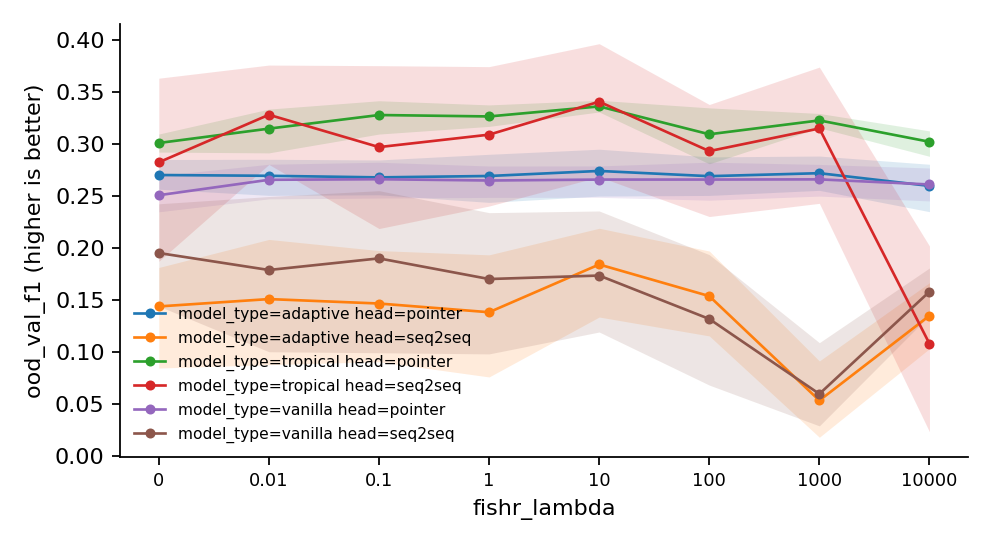
\includegraphics[width=\textwidth]{metric_ood_val_f1.png}
\caption{\texttt{ood\_val\_f1} against \texttt{fishr\_lambda}: the mean over seeds with a 95\% bootstrap CI, one line per combination of the other factors.}
\label{fig:ood_val_f1}
\end{figure}

{\small
\begin{longtable}{lllrlrrr}
\caption{\texttt{ood\_val\_f1} per cell: mean, 95\% bootstrap CI, SD, seeds, diverged runs.}\label{tab:summary-ood_val_f1}\\
\toprule
\texttt{model\_type} & \texttt{head} & \texttt{fishr\_lambda} & mean & 95\% CI & SD & $n$ & div.\\
\midrule
\endhead
adaptive & pointer & 0 & 0.2702 & [0.257, 0.285] & 0.0182 & 5 & 0\\
adaptive & pointer & 0.01 & 0.2695 & [0.251, 0.285] & 0.0218 & 5 & 0\\
adaptive & pointer & 0.1 & 0.268 & [0.251, 0.285] & 0.0217 & 5 & 0\\
adaptive & pointer & 1 & 0.2693 & [0.244, 0.29] & 0.0293 & 5 & 0\\
adaptive & pointer & 10 & 0.2742 & [0.25, 0.295] & 0.0291 & 5 & 0\\
adaptive & pointer & 100 & 0.2691 & [0.251, 0.288] & 0.0238 & 5 & 0\\
adaptive & pointer & 1000 & 0.272 & [0.255, 0.289] & 0.0212 & 5 & 0\\
adaptive & pointer & 1e+04 & 0.2598 & [0.235, 0.281] & 0.0287 & 5 & 0\\
adaptive & seq2seq & 0 & 0.1438 & [0.0846, 0.181] & 0.0655 & 5 & 0\\
adaptive & seq2seq & 0.01 & 0.1509 & [0.0878, 0.208] & 0.0766 & 5 & 0\\
adaptive & seq2seq & 0.1 & 0.1466 & [0.0906, 0.198] & 0.0689 & 5 & 0\\
adaptive & seq2seq & 1 & 0.1382 & [0.076, 0.193] & 0.0746 & 5 & 0\\
adaptive & seq2seq & 10 & 0.1842 & [0.134, 0.219] & 0.0561 & 5 & 0\\
adaptive & seq2seq & 100 & 0.1538 & [0.115, 0.197] & 0.0538 & 5 & 0\\
adaptive & seq2seq & 1000 & 0.05334 & [0.018, 0.0913] & 0.0494 & 5 & 0\\
adaptive & seq2seq & 1e+04 & 0.1349 & [0.103, 0.167] & 0.0405 & 5 & 0\\
tropical & pointer & 0 & 0.301 & [0.292, 0.31] & 0.0113 & 5 & 0\\
tropical & pointer & 0.01 & 0.3149 & [0.292, 0.334] & 0.0264 & 5 & 0\\
tropical & pointer & 0.1 & 0.3279 & [0.31, 0.342] & 0.0217 & 5 & 0\\
tropical & pointer & 1 & 0.3266 & [0.317, 0.338] & 0.0138 & 5 & 0\\
tropical & pointer & 10 & 0.3362 & [0.331, 0.342] & 0.00739 & 5 & 0\\
tropical & pointer & 100 & 0.3094 & [0.281, 0.335] & 0.0379 & 5 & 0\\
tropical & pointer & 1000 & 0.3228 & [0.316, 0.329] & 0.00862 & 5 & 0\\
tropical & pointer & 1e+04 & 0.3022 & [0.288, 0.313] & 0.0164 & 5 & 0\\
tropical & seq2seq & 0 & 0.2825 & [0.187, 0.363] & 0.112 & 5 & 0\\
tropical & seq2seq & 0.01 & 0.3282 & [0.28, 0.376] & 0.0629 & 5 & 0\\
tropical & seq2seq & 0.1 & 0.2971 & [0.219, 0.375] & 0.1 & 5 & 0\\
tropical & seq2seq & 1 & 0.3091 & [0.24, 0.374] & 0.0846 & 5 & 0\\
tropical & seq2seq & 10 & 0.3408 & [0.269, 0.397] & 0.0839 & 5 & 0\\
tropical & seq2seq & 100 & 0.2932 & [0.23, 0.338] & 0.0747 & 5 & 0\\
tropical & seq2seq & 1000 & 0.315 & [0.243, 0.374] & 0.0822 & 5 & 0\\
tropical & seq2seq & 1e+04 & 0.108 & [0.0233, 0.202] & 0.116 & 5 & 0\\
vanilla & pointer & 0 & 0.2508 & [0.235, 0.27] & 0.0228 & 5 & 0\\
vanilla & pointer & 0.01 & 0.2656 & [0.247, 0.281] & 0.0208 & 5 & 0\\
vanilla & pointer & 0.1 & 0.2662 & [0.248, 0.283] & 0.0221 & 5 & 0\\
vanilla & pointer & 1 & 0.265 & [0.249, 0.279] & 0.0197 & 5 & 0\\
vanilla & pointer & 10 & 0.2658 & [0.249, 0.279] & 0.0189 & 5 & 0\\
vanilla & pointer & 100 & 0.2659 & [0.246, 0.283] & 0.0234 & 5 & 0\\
vanilla & pointer & 1000 & 0.2661 & [0.25, 0.28] & 0.0193 & 5 & 0\\
vanilla & pointer & 1e+04 & 0.2611 & [0.245, 0.277] & 0.0213 & 5 & 0\\
vanilla & seq2seq & 0 & 0.1952 & [0.144, 0.243] & 0.0651 & 5 & 0\\
vanilla & seq2seq & 0.01 & 0.1789 & [0.1, 0.25] & 0.103 & 5 & 0\\
vanilla & seq2seq & 0.1 & 0.19 & [0.0993, 0.255] & 0.103 & 5 & 0\\
vanilla & seq2seq & 1 & 0.1702 & [0.0982, 0.234] & 0.0877 & 5 & 0\\
vanilla & seq2seq & 10 & 0.1735 & [0.119, 0.236] & 0.0734 & 5 & 0\\
vanilla & seq2seq & 100 & 0.1318 & [0.0682, 0.194] & 0.0795 & 5 & 0\\
vanilla & seq2seq & 1000 & 0.05965 & [0.0289, 0.109] & 0.0536 & 5 & 0\\
vanilla & seq2seq & 1e+04 & 0.158 & [0.135, 0.181] & 0.0287 & 5 & 0\\
\bottomrule
\end{longtable}
}

{\small
\begin{longtable}{lllrrrl}
\caption{\texttt{ood\_val\_f1}: each level of \texttt{fishr\_lambda} against its control (0), within each combination of the other factors. parametric: Dunnett vs control.}\label{tab:control-ood_val_f1}\\
\toprule
\texttt{model\_type} & \texttt{head} & \texttt{fishr\_lambda} & difference & 95\% CI & $p$ & \\
\midrule
\endhead
adaptive & pointer & 0.01 & $-7.575\times10^{-4}$ & [-0.0437, 0.0422] & 1.0000 & \\
adaptive & pointer & 0.1 & -0.00227 & [-0.0452, 0.0406] & 1.0000 & \\
adaptive & pointer & 1 & $-9.359\times10^{-4}$ & [-0.0439, 0.042] & 1.0000 & \\
adaptive & pointer & 10 & 0.00391 & [-0.039, 0.0468] & 0.9999 & \\
adaptive & pointer & 100 & -0.001113 & [-0.044, 0.0418] & 1.0000 & \\
adaptive & pointer & 1000 & 0.001751 & [-0.0412, 0.0447] & 1.0000 & \\
adaptive & pointer & 1e+04 & -0.01047 & [-0.0534, 0.0324] & 0.9756 & \\
adaptive & seq2seq & 0.01 & 0.007075 & [-0.101, 0.115] & 1.0000 & \\
adaptive & seq2seq & 0.1 & 0.002804 & [-0.105, 0.111] & 1.0000 & \\
adaptive & seq2seq & 1 & -0.005578 & [-0.114, 0.102] & 1.0000 & \\
adaptive & seq2seq & 10 & 0.04037 & [-0.0676, 0.148] & 0.8362 & \\
adaptive & seq2seq & 100 & 0.00994 & [-0.0981, 0.118] & 0.9999 & \\
adaptive & seq2seq & 1000 & -0.09048 & [-0.198, 0.0175] & 0.1308 & \\
adaptive & seq2seq & 1e+04 & -0.008894 & [-0.117, 0.0991] & 1.0000 & \\
tropical & pointer & 0.01 & 0.01381 & [-0.0218, 0.0494] & 0.8123 & \\
tropical & pointer & 0.1 & 0.0269 & [-0.00869, 0.0625] & 0.2023 & \\
tropical & pointer & 1 & 0.02554 & [-0.01, 0.0611] & 0.2450 & \\
tropical & pointer & 10 & 0.03519 & [$-3.97\times10^{-4}$, 0.0708] & 0.0537 & \\
tropical & pointer & 100 & 0.008386 & [-0.0272, 0.044] & 0.9796 & \\
tropical & pointer & 1000 & 0.02173 & [-0.0139, 0.0573] & 0.3982 & \\
tropical & pointer & 1e+04 & 0.001163 & [-0.0344, 0.0368] & 1.0000 & \\
tropical & seq2seq & 0.01 & 0.04574 & [-0.114, 0.205] & 0.9456 & \\
tropical & seq2seq & 0.1 & 0.01462 & [-0.145, 0.174] & 0.9999 & \\
tropical & seq2seq & 1 & 0.0266 & [-0.133, 0.186] & 0.9971 & \\
tropical & seq2seq & 10 & 0.05831 & [-0.101, 0.218] & 0.8485 & \\
tropical & seq2seq & 100 & 0.01078 & [-0.149, 0.17] & 1.0000 & \\
tropical & seq2seq & 1000 & 0.03254 & [-0.127, 0.192] & 0.9907 & \\
tropical & seq2seq & 1e+04 & -0.1745 & [-0.334, -0.0152] & 0.0271 & *\\
vanilla & pointer & 0.01 & 0.01484 & [-0.022, 0.0517] & 0.7872 & \\
vanilla & pointer & 0.1 & 0.01538 & [-0.0215, 0.0522] & 0.7609 & \\
vanilla & pointer & 1 & 0.01415 & [-0.0227, 0.051] & 0.8195 & \\
vanilla & pointer & 10 & 0.01503 & [-0.0218, 0.0519] & 0.7780 & \\
vanilla & pointer & 100 & 0.01507 & [-0.0218, 0.0519] & 0.7761 & \\
vanilla & pointer & 1000 & 0.01524 & [-0.0216, 0.0521] & 0.7675 & \\
vanilla & pointer & 1e+04 & 0.01033 & [-0.0265, 0.0472] & 0.9514 & \\
vanilla & seq2seq & 0.01 & -0.01634 & [-0.152, 0.12] & 0.9996 & \\
vanilla & seq2seq & 0.1 & -0.005171 & [-0.141, 0.131] & 1.0000 & \\
vanilla & seq2seq & 1 & -0.02504 & [-0.161, 0.111] & 0.9949 & \\
vanilla & seq2seq & 10 & -0.02168 & [-0.158, 0.114] & 0.9978 & \\
vanilla & seq2seq & 100 & -0.06344 & [-0.199, 0.0726] & 0.6671 & \\
vanilla & seq2seq & 1000 & -0.1356 & [-0.272, $4.57\times10^{-4}$] & 0.0510 & \\
vanilla & seq2seq & 1e+04 & -0.03718 & [-0.173, 0.0989] & 0.9569 & \\
\bottomrule
\end{longtable}
}

{\small
\begin{longtable}{llrrrrr}
\caption{\texttt{ood\_val\_f1} against log10 \texttt{fishr\_lambda}: parametric: OLS slope t-test, seed-bootstrap CI, with the Jonckheere--Terpstra ordered-trend $\tau$ and $p$.}\label{tab:trend-ood_val_f1}\\
\toprule
\texttt{model\_type} & \texttt{head} & estimate & 95\% CI & $p$ & JT $\tau$ & JT $p$\\
\midrule
\endhead
adaptive & pointer & $-7.598\times10^{-4}$ & [-0.00131, $-2.05\times10^{-4}$] & 0.7068 & -0.0171 & 0.9054\\
adaptive & seq2seq & -0.00782 & [-0.0189, 0.00525] & 0.1729 & -0.192 & 0.1566\\
tropical & pointer & -0.002338 & [-0.00405, $-1.58\times10^{-4}$] & 0.2203 & -0.238 & 0.0746\\
tropical & seq2seq & -0.02288 & [-0.0348, -0.0128] & 0.0109 & -0.265 & 0.0450\\
vanilla & pointer & $-4.600\times10^{-4}$ & [-0.0012, $5.42\times10^{-4}$] & 0.7792 & -0.0286 & 0.8432\\
vanilla & seq2seq & -0.01292 & [-0.0241, 0.00418] & 0.0661 & -0.238 & 0.0736\\
\bottomrule
\end{longtable}
}

{\small
\begin{longtable}{lrrrl}
\caption{\texttt{ood\_val\_f1}: paired contrasts by seed, Holm-corrected across the cells. parametric: paired t-test by seed, Holm.}\label{tab:paired-ood_val_f1}\\
\toprule
contrast (within) & difference & 95\% CI & $p$ & \\
\midrule
\endhead
\stackcell{model\_type: tropical - vanilla\\\footnotesize head=pointer fishr\_lambda=0 } & 0.05023 & [0.0216, 0.0788] & 0.0819 & \\
\stackcell{model\_type: tropical - vanilla\\\footnotesize head=pointer fishr\_lambda=0.01 } & 0.04921 & [0.0211, 0.0773] & 0.0819 & \\
\stackcell{model\_type: tropical - vanilla\\\footnotesize head=pointer fishr\_lambda=0.1 } & 0.06176 & [0.0226, 0.101] & 0.0829 & \\
\stackcell{model\_type: tropical - vanilla\\\footnotesize head=pointer fishr\_lambda=1 } & 0.06163 & [0.0333, 0.0899] & 0.0454 & *\\
\stackcell{model\_type: tropical - vanilla\\\footnotesize head=pointer fishr\_lambda=10 } & 0.0704 & [0.0471, 0.0937] & 0.0166 & *\\
\stackcell{model\_type: tropical - vanilla\\\footnotesize head=pointer fishr\_lambda=100 } & 0.04355 & [0.00532, 0.0818] & 0.1705 & \\
\stackcell{model\_type: tropical - vanilla\\\footnotesize head=pointer fishr\_lambda=1000 } & 0.05672 & [0.0319, 0.0815] & 0.0441 & *\\
\stackcell{model\_type: tropical - vanilla\\\footnotesize head=pointer fishr\_lambda=1e+04 } & 0.04107 & [0.00273, 0.0794] & 0.1705 & \\
\stackcell{model\_type: tropical - vanilla\\\footnotesize head=seq2seq fishr\_lambda=0 } & 0.08725 & [-0.0249, 0.199] & 0.1937 & \\
\stackcell{model\_type: tropical - vanilla\\\footnotesize head=seq2seq fishr\_lambda=0.01 } & 0.1493 & [0.0606, 0.238] & 0.0819 & \\
\stackcell{model\_type: tropical - vanilla\\\footnotesize head=seq2seq fishr\_lambda=0.1 } & 0.107 & [-0.00631, 0.22] & 0.1761 & \\
\stackcell{model\_type: tropical - vanilla\\\footnotesize head=seq2seq fishr\_lambda=1 } & 0.1389 & [0.0486, 0.229] & 0.0829 & \\
\stackcell{model\_type: tropical - vanilla\\\footnotesize head=seq2seq fishr\_lambda=10 } & 0.1672 & [0.0832, 0.251] & 0.0577 & \\
\stackcell{model\_type: tropical - vanilla\\\footnotesize head=seq2seq fishr\_lambda=100 } & 0.1615 & [0.109, 0.214] & 0.0162 & *\\
\stackcell{model\_type: tropical - vanilla\\\footnotesize head=seq2seq fishr\_lambda=1000 } & 0.2554 & [0.143, 0.368] & 0.0441 & *\\
\stackcell{model\_type: tropical - vanilla\\\footnotesize head=seq2seq fishr\_lambda=1e+04 } & -0.05008 & [-0.211, 0.111] & 0.4355 & \\
\stackcell{model\_type: adaptive - vanilla\\\footnotesize head=pointer fishr\_lambda=0 } & 0.01943 & [-0.00815, 0.047] & 1.0000 & \\
\stackcell{model\_type: adaptive - vanilla\\\footnotesize head=pointer fishr\_lambda=0.01 } & 0.003834 & [-0.0386, 0.0463] & 1.0000 & \\
\stackcell{model\_type: adaptive - vanilla\\\footnotesize head=pointer fishr\_lambda=0.1 } & 0.001782 & [-0.0421, 0.0457] & 1.0000 & \\
\stackcell{model\_type: adaptive - vanilla\\\footnotesize head=pointer fishr\_lambda=1 } & 0.004345 & [-0.0465, 0.0552] & 1.0000 & \\
\stackcell{model\_type: adaptive - vanilla\\\footnotesize head=pointer fishr\_lambda=10 } & 0.008312 & [-0.0443, 0.0609] & 1.0000 & \\
\stackcell{model\_type: adaptive - vanilla\\\footnotesize head=pointer fishr\_lambda=100 } & 0.003252 & [-0.0424, 0.0489] & 1.0000 & \\
\stackcell{model\_type: adaptive - vanilla\\\footnotesize head=pointer fishr\_lambda=1000 } & 0.005938 & [-0.034, 0.0459] & 1.0000 & \\
\stackcell{model\_type: adaptive - vanilla\\\footnotesize head=pointer fishr\_lambda=1e+04 } & -0.001369 & [-0.056, 0.0533] & 1.0000 & \\
\stackcell{model\_type: adaptive - vanilla\\\footnotesize head=seq2seq fishr\_lambda=0 } & -0.0514 & [-0.114, 0.0115] & 1.0000 & \\
\stackcell{model\_type: adaptive - vanilla\\\footnotesize head=seq2seq fishr\_lambda=0.01 } & -0.02798 & [-0.124, 0.0679] & 1.0000 & \\
\stackcell{model\_type: adaptive - vanilla\\\footnotesize head=seq2seq fishr\_lambda=0.1 } & -0.04342 & [-0.135, 0.0483] & 1.0000 & \\
\stackcell{model\_type: adaptive - vanilla\\\footnotesize head=seq2seq fishr\_lambda=1 } & -0.03194 & [-0.0932, 0.0293] & 1.0000 & \\
\stackcell{model\_type: adaptive - vanilla\\\footnotesize head=seq2seq fishr\_lambda=10 } & 0.01065 & [-0.0511, 0.0724] & 1.0000 & \\
\stackcell{model\_type: adaptive - vanilla\\\footnotesize head=seq2seq fishr\_lambda=100 } & 0.02198 & [-0.0579, 0.102] & 1.0000 & \\
\stackcell{model\_type: adaptive - vanilla\\\footnotesize head=seq2seq fishr\_lambda=1000 } & -0.006307 & [-0.0316, 0.019] & 1.0000 & \\
\stackcell{model\_type: adaptive - vanilla\\\footnotesize head=seq2seq fishr\_lambda=1e+04 } & -0.02312 & [-0.0426, -0.00359] & 0.4850 & \\
\stackcell{head: pointer - seq2seq\\\footnotesize model\_type=adaptive fishr\_lambda=0 } & 0.1264 & [0.0461, 0.207] & 0.2277 & \\
\stackcell{head: pointer - seq2seq\\\footnotesize model\_type=adaptive fishr\_lambda=0.01 } & 0.1186 & [0.0311, 0.206] & 0.2778 & \\
\stackcell{head: pointer - seq2seq\\\footnotesize model\_type=adaptive fishr\_lambda=0.1 } & 0.1213 & [0.0395, 0.203] & 0.2469 & \\
\stackcell{head: pointer - seq2seq\\\footnotesize model\_type=adaptive fishr\_lambda=1 } & 0.1311 & [0.0505, 0.212] & 0.2139 & \\
\stackcell{head: pointer - seq2seq\\\footnotesize model\_type=adaptive fishr\_lambda=10 } & 0.08997 & [0.0449, 0.135] & 0.1087 & \\
\stackcell{head: pointer - seq2seq\\\footnotesize model\_type=adaptive fishr\_lambda=100 } & 0.1154 & [0.0378, 0.193] & 0.2469 & \\
\stackcell{head: pointer - seq2seq\\\footnotesize model\_type=adaptive fishr\_lambda=1000 } & 0.2187 & [0.149, 0.288] & 0.0217 & *\\
\stackcell{head: pointer - seq2seq\\\footnotesize model\_type=adaptive fishr\_lambda=1e+04 } & 0.1248 & [0.0427, 0.207] & 0.2422 & \\
\stackcell{head: pointer - seq2seq\\\footnotesize model\_type=tropical fishr\_lambda=0 } & 0.01858 & [-0.122, 0.159] & 1.0000 & \\
\stackcell{head: pointer - seq2seq\\\footnotesize model\_type=tropical fishr\_lambda=0.01 } & -0.01334 & [-0.109, 0.082] & 1.0000 & \\
\stackcell{head: pointer - seq2seq\\\footnotesize model\_type=tropical fishr\_lambda=0.1 } & 0.03086 & [-0.115, 0.177] & 1.0000 & \\
\stackcell{head: pointer - seq2seq\\\footnotesize model\_type=tropical fishr\_lambda=1 } & 0.01752 & [-0.0874, 0.122] & 1.0000 & \\
\stackcell{head: pointer - seq2seq\\\footnotesize model\_type=tropical fishr\_lambda=10 } & -0.004535 & [-0.109, 0.0998] & 1.0000 & \\
\stackcell{head: pointer - seq2seq\\\footnotesize model\_type=tropical fishr\_lambda=100 } & 0.01619 & [-0.105, 0.138] & 1.0000 & \\
\stackcell{head: pointer - seq2seq\\\footnotesize model\_type=tropical fishr\_lambda=1000 } & 0.007765 & [-0.0968, 0.112] & 1.0000 & \\
\stackcell{head: pointer - seq2seq\\\footnotesize model\_type=tropical fishr\_lambda=1e+04 } & 0.1943 & [0.0537, 0.335] & 0.2778 & \\
\stackcell{head: pointer - seq2seq\\\footnotesize model\_type=vanilla fishr\_lambda=0 } & 0.0556 & [-0.0222, 0.133] & 1.0000 & \\
\stackcell{head: pointer - seq2seq\\\footnotesize model\_type=vanilla fishr\_lambda=0.01 } & 0.08678 & [-0.0478, 0.221] & 1.0000 & \\
\stackcell{head: pointer - seq2seq\\\footnotesize model\_type=vanilla fishr\_lambda=0.1 } & 0.07614 & [-0.0637, 0.216] & 1.0000 & \\
\stackcell{head: pointer - seq2seq\\\footnotesize model\_type=vanilla fishr\_lambda=1 } & 0.09478 & [-0.0319, 0.221] & 1.0000 & \\
\stackcell{head: pointer - seq2seq\\\footnotesize model\_type=vanilla fishr\_lambda=10 } & 0.09231 & [-0.0166, 0.201] & 0.9382 & \\
\stackcell{head: pointer - seq2seq\\\footnotesize model\_type=vanilla fishr\_lambda=100 } & 0.1341 & [0.013, 0.255] & 0.4826 & \\
\stackcell{head: pointer - seq2seq\\\footnotesize model\_type=vanilla fishr\_lambda=1000 } & 0.2064 & [0.12, 0.293] & 0.0585 & \\
\stackcell{head: pointer - seq2seq\\\footnotesize model\_type=vanilla fishr\_lambda=1e+04 } & 0.1031 & [0.0794, 0.127] & 0.0065 & *\\
\bottomrule
\end{longtable}
}

\subsection{\texttt{ood\_val\_exact}}
\begin{figure}[tbp]
\centering
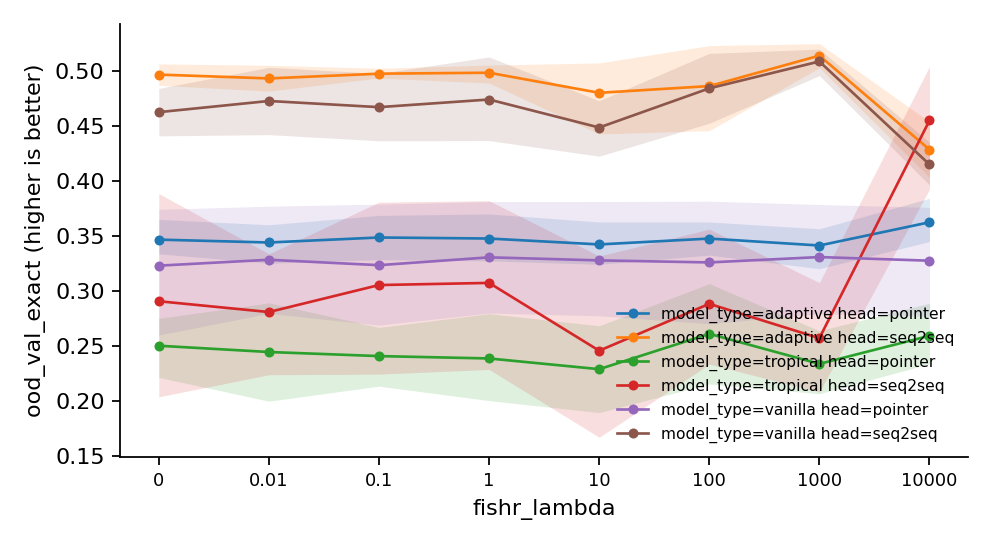
\includegraphics[width=\textwidth]{metric_ood_val_exact.png}
\caption{\texttt{ood\_val\_exact} against \texttt{fishr\_lambda}: the mean over seeds with a 95\% bootstrap CI, one line per combination of the other factors.}
\label{fig:ood_val_exact}
\end{figure}

{\small
\begin{longtable}{lllrlrrr}
\caption{\texttt{ood\_val\_exact} per cell: mean, 95\% bootstrap CI, SD, seeds, diverged runs.}\label{tab:summary-ood_val_exact}\\
\toprule
\texttt{model\_type} & \texttt{head} & \texttt{fishr\_lambda} & mean & 95\% CI & SD & $n$ & div.\\
\midrule
\endhead
adaptive & pointer & 0 & 0.3467 & [0.334, 0.365] & 0.0209 & 5 & 0\\
adaptive & pointer & 0.01 & 0.3441 & [0.325, 0.36] & 0.0231 & 5 & 0\\
adaptive & pointer & 0.1 & 0.3487 & [0.329, 0.369] & 0.0281 & 5 & 0\\
adaptive & pointer & 1 & 0.3477 & [0.327, 0.37] & 0.0287 & 5 & 0\\
adaptive & pointer & 10 & 0.3424 & [0.324, 0.363] & 0.0245 & 5 & 0\\
adaptive & pointer & 100 & 0.3477 & [0.333, 0.363] & 0.0202 & 5 & 0\\
adaptive & pointer & 1000 & 0.3414 & [0.32, 0.357] & 0.0246 & 5 & 0\\
adaptive & pointer & 1e+04 & 0.3625 & [0.345, 0.384] & 0.0257 & 5 & 0\\
adaptive & seq2seq & 0 & 0.4971 & [0.487, 0.507] & 0.013 & 5 & 0\\
adaptive & seq2seq & 0.01 & 0.4936 & [0.482, 0.506] & 0.015 & 5 & 0\\
adaptive & seq2seq & 0.1 & 0.498 & [0.494, 0.503] & 0.00558 & 5 & 0\\
adaptive & seq2seq & 1 & 0.4988 & [0.489, 0.506] & 0.0115 & 5 & 0\\
adaptive & seq2seq & 10 & 0.4805 & [0.443, 0.508] & 0.0418 & 5 & 0\\
adaptive & seq2seq & 100 & 0.4867 & [0.446, 0.524] & 0.0493 & 5 & 0\\
adaptive & seq2seq & 1000 & 0.5144 & [0.503, 0.525] & 0.0141 & 5 & 0\\
adaptive & seq2seq & 1e+04 & 0.4288 & [0.403, 0.454] & 0.0359 & 5 & 0\\
tropical & pointer & 0 & 0.25 & [0.221, 0.275] & 0.0347 & 5 & 0\\
tropical & pointer & 0.01 & 0.2443 & [0.2, 0.289] & 0.0587 & 5 & 0\\
tropical & pointer & 0.1 & 0.2406 & [0.213, 0.267] & 0.0351 & 5 & 0\\
tropical & pointer & 1 & 0.2384 & [0.2, 0.279] & 0.0522 & 5 & 0\\
tropical & pointer & 10 & 0.2287 & [0.189, 0.268] & 0.0512 & 5 & 0\\
tropical & pointer & 100 & 0.2609 & [0.215, 0.307] & 0.061 & 5 & 0\\
tropical & pointer & 1000 & 0.2335 & [0.206, 0.264] & 0.037 & 5 & 0\\
tropical & pointer & 1e+04 & 0.2591 & [0.234, 0.289] & 0.0354 & 5 & 0\\
tropical & seq2seq & 0 & 0.2906 & [0.204, 0.389] & 0.119 & 5 & 0\\
tropical & seq2seq & 0.01 & 0.2807 & [0.224, 0.334] & 0.0722 & 5 & 0\\
tropical & seq2seq & 0.1 & 0.3053 & [0.224, 0.381] & 0.101 & 5 & 0\\
tropical & seq2seq & 1 & 0.3073 & [0.228, 0.382] & 0.102 & 5 & 0\\
tropical & seq2seq & 10 & 0.2455 & [0.167, 0.332] & 0.105 & 5 & 0\\
tropical & seq2seq & 100 & 0.2882 & [0.233, 0.356] & 0.0793 & 5 & 0\\
tropical & seq2seq & 1000 & 0.2569 & [0.208, 0.308] & 0.0649 & 5 & 0\\
tropical & seq2seq & 1e+04 & 0.4553 & [0.393, 0.505] & 0.0735 & 5 & 0\\
vanilla & pointer & 0 & 0.323 & [0.26, 0.374] & 0.0749 & 5 & 0\\
vanilla & pointer & 0.01 & 0.3284 & [0.28, 0.377] & 0.0651 & 5 & 0\\
vanilla & pointer & 0.1 & 0.3235 & [0.269, 0.379] & 0.07 & 5 & 0\\
vanilla & pointer & 1 & 0.3306 & [0.28, 0.381] & 0.0672 & 5 & 0\\
vanilla & pointer & 10 & 0.3278 & [0.277, 0.381] & 0.067 & 5 & 0\\
vanilla & pointer & 100 & 0.326 & [0.27, 0.382] & 0.0724 & 5 & 0\\
vanilla & pointer & 1000 & 0.3308 & [0.279, 0.379] & 0.0653 & 5 & 0\\
vanilla & pointer & 1e+04 & 0.3275 & [0.277, 0.376] & 0.0666 & 5 & 0\\
vanilla & seq2seq & 0 & 0.4629 & [0.441, 0.485] & 0.0288 & 5 & 0\\
vanilla & seq2seq & 0.01 & 0.4731 & [0.442, 0.504] & 0.0405 & 5 & 0\\
vanilla & seq2seq & 0.1 & 0.4675 & [0.437, 0.498] & 0.0407 & 5 & 0\\
vanilla & seq2seq & 1 & 0.4744 & [0.437, 0.513] & 0.0468 & 5 & 0\\
vanilla & seq2seq & 10 & 0.4489 & [0.423, 0.473] & 0.0325 & 5 & 0\\
vanilla & seq2seq & 100 & 0.4846 & [0.453, 0.516] & 0.0425 & 5 & 0\\
vanilla & seq2seq & 1000 & 0.5091 & [0.496, 0.52] & 0.016 & 5 & 0\\
vanilla & seq2seq & 1e+04 & 0.4152 & [0.397, 0.435] & 0.0248 & 5 & 0\\
\bottomrule
\end{longtable}
}

{\small
\begin{longtable}{lllrrrl}
\caption{\texttt{ood\_val\_exact}: each level of \texttt{fishr\_lambda} against its control (0), within each combination of the other factors. parametric: Dunnett vs control.}\label{tab:control-ood_val_exact}\\
\toprule
\texttt{model\_type} & \texttt{head} & \texttt{fishr\_lambda} & difference & 95\% CI & $p$ & \\
\midrule
\endhead
adaptive & pointer & 0.01 & -0.00262 & [-0.0457, 0.0404] & 1.0000 & \\
adaptive & pointer & 0.1 & 0.00194 & [-0.0411, 0.045] & 1.0000 & \\
adaptive & pointer & 1 & 0.001 & [-0.0421, 0.0441] & 1.0000 & \\
adaptive & pointer & 10 & -0.00438 & [-0.0474, 0.0387] & 0.9999 & \\
adaptive & pointer & 100 & $9.600\times10^{-4}$ & [-0.0421, 0.044] & 1.0000 & \\
adaptive & pointer & 1000 & -0.00536 & [-0.0484, 0.0377] & 0.9995 & \\
adaptive & pointer & 1e+04 & 0.0158 & [-0.0273, 0.0589] & 0.8469 & \\
adaptive & seq2seq & 0.01 & -0.00348 & [-0.0522, 0.0452] & 1.0000 & \\
adaptive & seq2seq & 0.1 & $8.400\times10^{-4}$ & [-0.0479, 0.0496] & 1.0000 & \\
adaptive & seq2seq & 1 & 0.0017 & [-0.047, 0.0504] & 1.0000 & \\
adaptive & seq2seq & 10 & -0.0166 & [-0.0653, 0.0321] & 0.8853 & \\
adaptive & seq2seq & 100 & -0.01046 & [-0.0592, 0.0383] & 0.9877 & \\
adaptive & seq2seq & 1000 & 0.01728 & [-0.0314, 0.066] & 0.8656 & \\
adaptive & seq2seq & 1e+04 & -0.06832 & [-0.117, -0.0196] & 0.0031 & *\\
tropical & pointer & 0.01 & -0.00572 & [-0.0876, 0.0761] & 1.0000 & \\
tropical & pointer & 0.1 & -0.00944 & [-0.0913, 0.0724] & 0.9997 & \\
tropical & pointer & 1 & -0.0116 & [-0.0935, 0.0703] & 0.9990 & \\
tropical & pointer & 10 & -0.02136 & [-0.103, 0.0605] & 0.9656 & \\
tropical & pointer & 100 & 0.01084 & [-0.071, 0.0927] & 0.9993 & \\
tropical & pointer & 1000 & -0.01654 & [-0.0984, 0.0653] & 0.9912 & \\
tropical & pointer & 1e+04 & 0.00906 & [-0.0728, 0.0909] & 0.9998 & \\
tropical & seq2seq & 0.01 & -0.00986 & [-0.17, 0.15] & 1.0000 & \\
tropical & seq2seq & 0.1 & 0.01474 & [-0.145, 0.175] & 0.9999 & \\
tropical & seq2seq & 1 & 0.0167 & [-0.143, 0.177] & 0.9999 & \\
tropical & seq2seq & 10 & -0.04508 & [-0.205, 0.115] & 0.9498 & \\
tropical & seq2seq & 100 & -0.00238 & [-0.162, 0.157] & 1.0000 & \\
tropical & seq2seq & 1000 & -0.03368 & [-0.193, 0.126] & 0.9889 & \\
tropical & seq2seq & 1e+04 & 0.1647 & [0.0049, 0.325] & 0.0413 & *\\
vanilla & pointer & 0.01 & 0.00536 & [-0.115, 0.125] & 1.0000 & \\
vanilla & pointer & 0.1 & $4.400\times10^{-4}$ & [-0.119, 0.12] & 1.0000 & \\
vanilla & pointer & 1 & 0.00758 & [-0.112, 0.127] & 1.0000 & \\
vanilla & pointer & 10 & 0.0048 & [-0.115, 0.125] & 1.0000 & \\
vanilla & pointer & 100 & 0.00294 & [-0.117, 0.123] & 1.0000 & \\
vanilla & pointer & 1000 & 0.00782 & [-0.112, 0.128] & 1.0000 & \\
vanilla & pointer & 1e+04 & 0.00452 & [-0.115, 0.124] & 1.0000 & \\
vanilla & seq2seq & 0.01 & 0.01018 & [-0.0517, 0.0721] & 0.9974 & \\
vanilla & seq2seq & 0.1 & 0.00456 & [-0.0574, 0.0665] & 1.0000 & \\
vanilla & seq2seq & 1 & 0.01152 & [-0.0504, 0.0734] & 0.9946 & \\
vanilla & seq2seq & 10 & -0.014 & [-0.0759, 0.0479] & 0.9837 & \\
vanilla & seq2seq & 100 & 0.0217 & [-0.0402, 0.0836] & 0.8717 & \\
vanilla & seq2seq & 1000 & 0.0462 & [-0.0157, 0.108] & 0.2128 & \\
vanilla & seq2seq & 1e+04 & -0.04768 & [-0.11, 0.0142] & 0.1883 & \\
\bottomrule
\end{longtable}
}

{\small
\begin{longtable}{llrrrrr}
\caption{\texttt{ood\_val\_exact} against log10 \texttt{fishr\_lambda}: parametric: OLS slope t-test, seed-bootstrap CI, with the Jonckheere--Terpstra ordered-trend $\tau$ and $p$.}\label{tab:trend-ood_val_exact}\\
\toprule
\texttt{model\_type} & \texttt{head} & estimate & 95\% CI & $p$ & JT $\tau$ & JT $p$\\
\midrule
\endhead
adaptive & pointer & 0.001451 & [$3.36\times10^{-4}$, 0.00215] & 0.4783 & 0.099 & 0.4517\\
adaptive & seq2seq & -0.006207 & [-0.00934, -0.00308] & 0.0455 & -0.124 & 0.3551\\
tropical & pointer & 0.001878 & [-0.00208, 0.00485] & 0.6314 & 0.0476 & 0.7267\\
tropical & seq2seq & 0.01456 & [0.00587, 0.0283] & 0.0934 & 0.177 & 0.1800\\
vanilla & pointer & $2.714\times10^{-4}$ & [$-8.26\times10^{-4}$, 0.00159] & 0.9593 & -0.00952 & 0.9516\\
vanilla & seq2seq & -0.002861 & [-0.00871, 0.00305] & 0.4391 & -0.0914 & 0.4887\\
\bottomrule
\end{longtable}
}

{\small
\begin{longtable}{lrrrl}
\caption{\texttt{ood\_val\_exact}: paired contrasts by seed, Holm-corrected across the cells. parametric: paired t-test by seed, Holm.}\label{tab:paired-ood_val_exact}\\
\toprule
contrast (within) & difference & 95\% CI & $p$ & \\
\midrule
\endhead
\stackcell{model\_type: tropical - vanilla\\\footnotesize head=pointer fishr\_lambda=0 } & -0.07298 & [-0.206, 0.0602] & 0.5887 & \\
\stackcell{model\_type: tropical - vanilla\\\footnotesize head=pointer fishr\_lambda=0.01 } & -0.08406 & [-0.186, 0.018] & 0.5576 & \\
\stackcell{model\_type: tropical - vanilla\\\footnotesize head=pointer fishr\_lambda=0.1 } & -0.08286 & [-0.168, 0.00239] & 0.4875 & \\
\stackcell{model\_type: tropical - vanilla\\\footnotesize head=pointer fishr\_lambda=1 } & -0.09216 & [-0.214, 0.0298] & 0.5576 & \\
\stackcell{model\_type: tropical - vanilla\\\footnotesize head=pointer fishr\_lambda=10 } & -0.09914 & [-0.216, 0.0174] & 0.5576 & \\
\stackcell{model\_type: tropical - vanilla\\\footnotesize head=pointer fishr\_lambda=100 } & -0.06508 & [-0.169, 0.0391] & 0.5887 & \\
\stackcell{model\_type: tropical - vanilla\\\footnotesize head=pointer fishr\_lambda=1000 } & -0.09734 & [-0.207, 0.0125] & 0.5576 & \\
\stackcell{model\_type: tropical - vanilla\\\footnotesize head=pointer fishr\_lambda=1e+04 } & -0.06844 & [-0.174, 0.0374] & 0.5887 & \\
\stackcell{model\_type: tropical - vanilla\\\footnotesize head=seq2seq fishr\_lambda=0 } & -0.1723 & [-0.295, -0.0493] & 0.1871 & \\
\stackcell{model\_type: tropical - vanilla\\\footnotesize head=seq2seq fishr\_lambda=0.01 } & -0.1923 & [-0.251, -0.133] & 0.0123 & *\\
\stackcell{model\_type: tropical - vanilla\\\footnotesize head=seq2seq fishr\_lambda=0.1 } & -0.1621 & [-0.271, -0.0534] & 0.1722 & \\
\stackcell{model\_type: tropical - vanilla\\\footnotesize head=seq2seq fishr\_lambda=1 } & -0.1671 & [-0.285, -0.0492] & 0.1871 & \\
\stackcell{model\_type: tropical - vanilla\\\footnotesize head=seq2seq fishr\_lambda=10 } & -0.2034 & [-0.327, -0.0799] & 0.1330 & \\
\stackcell{model\_type: tropical - vanilla\\\footnotesize head=seq2seq fishr\_lambda=100 } & -0.1964 & [-0.265, -0.127] & 0.0194 & *\\
\stackcell{model\_type: tropical - vanilla\\\footnotesize head=seq2seq fishr\_lambda=1000 } & -0.2522 & [-0.327, -0.178] & 0.0115 & *\\
\stackcell{model\_type: tropical - vanilla\\\footnotesize head=seq2seq fishr\_lambda=1e+04 } & 0.04008 & [-0.0672, 0.147] & 0.5887 & \\
\stackcell{model\_type: adaptive - vanilla\\\footnotesize head=pointer fishr\_lambda=0 } & 0.02372 & [-0.0918, 0.139] & 1.0000 & \\
\stackcell{model\_type: adaptive - vanilla\\\footnotesize head=pointer fishr\_lambda=0.01 } & 0.01574 & [-0.0832, 0.115] & 1.0000 & \\
\stackcell{model\_type: adaptive - vanilla\\\footnotesize head=pointer fishr\_lambda=0.1 } & 0.02522 & [-0.0713, 0.122] & 1.0000 & \\
\stackcell{model\_type: adaptive - vanilla\\\footnotesize head=pointer fishr\_lambda=1 } & 0.01714 & [-0.0923, 0.127] & 1.0000 & \\
\stackcell{model\_type: adaptive - vanilla\\\footnotesize head=pointer fishr\_lambda=10 } & 0.01454 & [-0.0949, 0.124] & 1.0000 & \\
\stackcell{model\_type: adaptive - vanilla\\\footnotesize head=pointer fishr\_lambda=100 } & 0.02174 & [-0.0741, 0.118] & 1.0000 & \\
\stackcell{model\_type: adaptive - vanilla\\\footnotesize head=pointer fishr\_lambda=1000 } & 0.01054 & [-0.0922, 0.113] & 1.0000 & \\
\stackcell{model\_type: adaptive - vanilla\\\footnotesize head=pointer fishr\_lambda=1e+04 } & 0.035 & [-0.0718, 0.142] & 1.0000 & \\
\stackcell{model\_type: adaptive - vanilla\\\footnotesize head=seq2seq fishr\_lambda=0 } & 0.03422 & [-0.00104, 0.0695] & 0.8702 & \\
\stackcell{model\_type: adaptive - vanilla\\\footnotesize head=seq2seq fishr\_lambda=0.01 } & 0.02056 & [-0.0323, 0.0734] & 1.0000 & \\
\stackcell{model\_type: adaptive - vanilla\\\footnotesize head=seq2seq fishr\_lambda=0.1 } & 0.0305 & [-0.0256, 0.0866] & 1.0000 & \\
\stackcell{model\_type: adaptive - vanilla\\\footnotesize head=seq2seq fishr\_lambda=1 } & 0.0244 & [-0.0352, 0.084] & 1.0000 & \\
\stackcell{model\_type: adaptive - vanilla\\\footnotesize head=seq2seq fishr\_lambda=10 } & 0.03162 & [-0.0162, 0.0794] & 1.0000 & \\
\stackcell{model\_type: adaptive - vanilla\\\footnotesize head=seq2seq fishr\_lambda=100 } & 0.00206 & [-0.0562, 0.0603] & 1.0000 & \\
\stackcell{model\_type: adaptive - vanilla\\\footnotesize head=seq2seq fishr\_lambda=1000 } & 0.0053 & [-0.00838, 0.019] & 1.0000 & \\
\stackcell{model\_type: adaptive - vanilla\\\footnotesize head=seq2seq fishr\_lambda=1e+04 } & 0.01358 & [-0.00377, 0.0309] & 1.0000 & \\
\stackcell{head: pointer - seq2seq\\\footnotesize model\_type=adaptive fishr\_lambda=0 } & -0.1504 & [-0.19, -0.111] & 0.0090 & *\\
\stackcell{head: pointer - seq2seq\\\footnotesize model\_type=adaptive fishr\_lambda=0.01 } & -0.1495 & [-0.181, -0.118] & 0.0042 & *\\
\stackcell{head: pointer - seq2seq\\\footnotesize model\_type=adaptive fishr\_lambda=0.1 } & -0.1493 & [-0.181, -0.118] & 0.0043 & *\\
\stackcell{head: pointer - seq2seq\\\footnotesize model\_type=adaptive fishr\_lambda=1 } & -0.1511 & [-0.185, -0.117] & 0.0051 & *\\
\stackcell{head: pointer - seq2seq\\\footnotesize model\_type=adaptive fishr\_lambda=10 } & -0.1382 & [-0.201, -0.0751] & 0.0701 & \\
\stackcell{head: pointer - seq2seq\\\footnotesize model\_type=adaptive fishr\_lambda=100 } & -0.139 & [-0.211, -0.0672] & 0.0960 & \\
\stackcell{head: pointer - seq2seq\\\footnotesize model\_type=adaptive fishr\_lambda=1000 } & -0.173 & [-0.202, -0.144] & 0.0019 & *\\
\stackcell{head: pointer - seq2seq\\\footnotesize model\_type=adaptive fishr\_lambda=1e+04 } & -0.06626 & [-0.127, -0.00541] & 0.3124 & \\
\stackcell{head: pointer - seq2seq\\\footnotesize model\_type=tropical fishr\_lambda=0 } & -0.04056 & [-0.176, 0.0948] & 1.0000 & \\
\stackcell{head: pointer - seq2seq\\\footnotesize model\_type=tropical fishr\_lambda=0.01 } & -0.03642 & [-0.163, 0.0904] & 1.0000 & \\
\stackcell{head: pointer - seq2seq\\\footnotesize model\_type=tropical fishr\_lambda=0.1 } & -0.06474 & [-0.223, 0.0936] & 1.0000 & \\
\stackcell{head: pointer - seq2seq\\\footnotesize model\_type=tropical fishr\_lambda=1 } & -0.06886 & [-0.187, 0.0497] & 1.0000 & \\
\stackcell{head: pointer - seq2seq\\\footnotesize model\_type=tropical fishr\_lambda=10 } & -0.01684 & [-0.164, 0.131] & 1.0000 & \\
\stackcell{head: pointer - seq2seq\\\footnotesize model\_type=tropical fishr\_lambda=100 } & -0.02734 & [-0.193, 0.138] & 1.0000 & \\
\stackcell{head: pointer - seq2seq\\\footnotesize model\_type=tropical fishr\_lambda=1000 } & -0.02342 & [-0.121, 0.0738] & 1.0000 & \\
\stackcell{head: pointer - seq2seq\\\footnotesize model\_type=tropical fishr\_lambda=1e+04 } & -0.1962 & [-0.297, -0.0956] & 0.0960 & \\
\stackcell{head: pointer - seq2seq\\\footnotesize model\_type=vanilla fishr\_lambda=0 } & -0.1399 & [-0.234, -0.0461] & 0.2013 & \\
\stackcell{head: pointer - seq2seq\\\footnotesize model\_type=vanilla fishr\_lambda=0.01 } & -0.1447 & [-0.253, -0.0366] & 0.2465 & \\
\stackcell{head: pointer - seq2seq\\\footnotesize model\_type=vanilla fishr\_lambda=0.1 } & -0.144 & [-0.259, -0.0293] & 0.2773 & \\
\stackcell{head: pointer - seq2seq\\\footnotesize model\_type=vanilla fishr\_lambda=1 } & -0.1438 & [-0.266, -0.0217] & 0.2905 & \\
\stackcell{head: pointer - seq2seq\\\footnotesize model\_type=vanilla fishr\_lambda=10 } & -0.1211 & [-0.222, -0.0202] & 0.2905 & \\
\stackcell{head: pointer - seq2seq\\\footnotesize model\_type=vanilla fishr\_lambda=100 } & -0.1586 & [-0.26, -0.0576] & 0.1809 & \\
\stackcell{head: pointer - seq2seq\\\footnotesize model\_type=vanilla fishr\_lambda=1000 } & -0.1783 & [-0.268, -0.0889] & 0.0933 & \\
\stackcell{head: pointer - seq2seq\\\footnotesize model\_type=vanilla fishr\_lambda=1e+04 } & -0.08768 & [-0.15, -0.0258] & 0.2221 & \\
\bottomrule
\end{longtable}
}

\subsection{\texttt{ood\_noise\_f1}}
\begin{figure}[tbp]
\centering
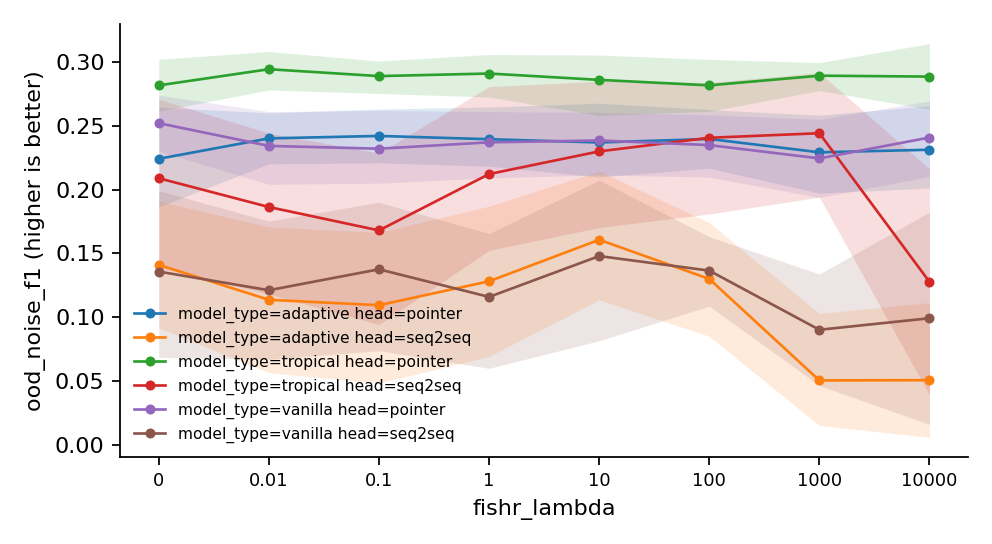
\includegraphics[width=\textwidth]{metric_ood_noise_f1.png}
\caption{\texttt{ood\_noise\_f1} against \texttt{fishr\_lambda}: the mean over seeds with a 95\% bootstrap CI, one line per combination of the other factors.}
\label{fig:ood_noise_f1}
\end{figure}

{\small
\begin{longtable}{lllrlrrr}
\caption{\texttt{ood\_noise\_f1} per cell: mean, 95\% bootstrap CI, SD, seeds, diverged runs.}\label{tab:summary-ood_noise_f1}\\
\toprule
\texttt{model\_type} & \texttt{head} & \texttt{fishr\_lambda} & mean & 95\% CI & SD & $n$ & div.\\
\midrule
\endhead
adaptive & pointer & 0 & 0.2241 & [0.186, 0.265] & 0.0488 & 5 & 0\\
adaptive & pointer & 0.01 & 0.2401 & [0.22, 0.26] & 0.0259 & 5 & 0\\
adaptive & pointer & 0.1 & 0.242 & [0.221, 0.263] & 0.0271 & 5 & 0\\
adaptive & pointer & 1 & 0.2395 & [0.218, 0.265] & 0.0295 & 5 & 0\\
adaptive & pointer & 10 & 0.2369 & [0.21, 0.268] & 0.0367 & 5 & 0\\
adaptive & pointer & 100 & 0.2397 & [0.217, 0.263] & 0.03 & 5 & 0\\
adaptive & pointer & 1000 & 0.2292 & [0.197, 0.258] & 0.0382 & 5 & 0\\
adaptive & pointer & 1e+04 & 0.2312 & [0.201, 0.266] & 0.0422 & 5 & 0\\
adaptive & seq2seq & 0 & 0.1409 & [0.0916, 0.191] & 0.0642 & 5 & 0\\
adaptive & seq2seq & 0.01 & 0.1135 & [0.0564, 0.171] & 0.0727 & 5 & 0\\
adaptive & seq2seq & 0.1 & 0.1093 & [0.0482, 0.166] & 0.0778 & 5 & 0\\
adaptive & seq2seq & 1 & 0.1281 & [0.0691, 0.187] & 0.0761 & 5 & 0\\
adaptive & seq2seq & 10 & 0.1606 & [0.113, 0.215] & 0.0652 & 5 & 0\\
adaptive & seq2seq & 100 & 0.1299 & [0.0849, 0.174] & 0.0579 & 5 & 0\\
adaptive & seq2seq & 1000 & 0.05033 & [0.015, 0.103] & 0.0616 & 5 & 0\\
adaptive & seq2seq & 1e+04 & 0.05052 & [0.00575, 0.111] & 0.0686 & 5 & 0\\
tropical & pointer & 0 & 0.2817 & [0.262, 0.302] & 0.0281 & 5 & 0\\
tropical & pointer & 0.01 & 0.2944 & [0.278, 0.308] & 0.0198 & 5 & 0\\
tropical & pointer & 0.1 & 0.289 & [0.275, 0.301] & 0.0157 & 5 & 0\\
tropical & pointer & 1 & 0.291 & [0.273, 0.306] & 0.0217 & 5 & 0\\
tropical & pointer & 10 & 0.286 & [0.258, 0.306] & 0.0315 & 5 & 0\\
tropical & pointer & 100 & 0.2817 & [0.261, 0.302] & 0.0257 & 5 & 0\\
tropical & pointer & 1000 & 0.2893 & [0.278, 0.3] & 0.0142 & 5 & 0\\
tropical & pointer & 1e+04 & 0.2886 & [0.263, 0.314] & 0.0331 & 5 & 0\\
tropical & seq2seq & 0 & 0.2089 & [0.139, 0.271] & 0.0844 & 5 & 0\\
tropical & seq2seq & 0.01 & 0.1863 & [0.118, 0.244] & 0.0825 & 5 & 0\\
tropical & seq2seq & 0.1 & 0.1679 & [0.0941, 0.229] & 0.0895 & 5 & 0\\
tropical & seq2seq & 1 & 0.2122 & [0.152, 0.281] & 0.0806 & 5 & 0\\
tropical & seq2seq & 10 & 0.2299 & [0.17, 0.285] & 0.0766 & 5 & 0\\
tropical & seq2seq & 100 & 0.2406 & [0.181, 0.284] & 0.0683 & 5 & 0\\
tropical & seq2seq & 1000 & 0.2442 & [0.194, 0.292] & 0.0662 & 5 & 0\\
tropical & seq2seq & 1e+04 & 0.1276 & [0.0389, 0.216] & 0.12 & 5 & 0\\
vanilla & pointer & 0 & 0.2521 & [0.23, 0.274] & 0.0299 & 5 & 0\\
vanilla & pointer & 0.01 & 0.2342 & [0.204, 0.261] & 0.0379 & 5 & 0\\
vanilla & pointer & 0.1 & 0.232 & [0.205, 0.262] & 0.0369 & 5 & 0\\
vanilla & pointer & 1 & 0.237 & [0.209, 0.261] & 0.0343 & 5 & 0\\
vanilla & pointer & 10 & 0.2385 & [0.211, 0.26] & 0.0329 & 5 & 0\\
vanilla & pointer & 100 & 0.2349 & [0.21, 0.259] & 0.0331 & 5 & 0\\
vanilla & pointer & 1000 & 0.2244 & [0.194, 0.255] & 0.0391 & 5 & 0\\
vanilla & pointer & 1e+04 & 0.2408 & [0.21, 0.27] & 0.0372 & 5 & 0\\
vanilla & seq2seq & 0 & 0.1357 & [0.0684, 0.199] & 0.0834 & 5 & 0\\
vanilla & seq2seq & 0.01 & 0.121 & [0.0669, 0.175] & 0.0713 & 5 & 0\\
vanilla & seq2seq & 0.1 & 0.1375 & [0.0736, 0.19] & 0.0761 & 5 & 0\\
vanilla & seq2seq & 1 & 0.1158 & [0.0598, 0.165] & 0.0673 & 5 & 0\\
vanilla & seq2seq & 10 & 0.1478 & [0.0814, 0.207] & 0.0844 & 5 & 0\\
vanilla & seq2seq & 100 & 0.1364 & [0.109, 0.163] & 0.0353 & 5 & 0\\
vanilla & seq2seq & 1000 & 0.09003 & [0.0463, 0.134] & 0.0558 & 5 & 0\\
vanilla & seq2seq & 1e+04 & 0.09908 & [0.0158, 0.182] & 0.108 & 5 & 0\\
\bottomrule
\end{longtable}
}

{\small
\begin{longtable}{lllrrrl}
\caption{\texttt{ood\_noise\_f1}: each level of \texttt{fishr\_lambda} against its control (0), within each combination of the other factors. parametric: Dunnett vs control.}\label{tab:control-ood_noise_f1}\\
\toprule
\texttt{model\_type} & \texttt{head} & \texttt{fishr\_lambda} & difference & 95\% CI & $p$ & \\
\midrule
\endhead
adaptive & pointer & 0.01 & 0.01601 & [-0.0462, 0.0782] & 0.9680 & \\
adaptive & pointer & 0.1 & 0.01792 & [-0.0443, 0.0802] & 0.9448 & \\
adaptive & pointer & 1 & 0.01537 & [-0.0469, 0.0776] & 0.9740 & \\
adaptive & pointer & 10 & 0.01279 & [-0.0494, 0.075] & 0.9904 & \\
adaptive & pointer & 100 & 0.01555 & [-0.0467, 0.0778] & 0.9724 & \\
adaptive & pointer & 1000 & 0.005084 & [-0.0571, 0.0673] & 1.0000 & \\
adaptive & pointer & 1e+04 & 0.007099 & [-0.0551, 0.0693] & 0.9997 & \\
adaptive & seq2seq & 0.01 & -0.02741 & [-0.147, 0.092] & 0.9823 & \\
adaptive & seq2seq & 0.1 & -0.03163 & [-0.151, 0.0878] & 0.9630 & \\
adaptive & seq2seq & 1 & -0.01289 & [-0.132, 0.107] & 0.9998 & \\
adaptive & seq2seq & 10 & 0.01967 & [-0.0997, 0.139] & 0.9974 & \\
adaptive & seq2seq & 100 & -0.01104 & [-0.13, 0.108] & 0.9999 & \\
adaptive & seq2seq & 1000 & -0.09062 & [-0.21, 0.0288] & 0.1992 & \\
adaptive & seq2seq & 1e+04 & -0.09043 & [-0.21, 0.029] & 0.2009 & \\
tropical & pointer & 0.01 & 0.01268 & [-0.0304, 0.0557] & 0.9386 & \\
tropical & pointer & 0.1 & 0.00728 & [-0.0358, 0.0503] & 0.9969 & \\
tropical & pointer & 1 & 0.009293 & [-0.0337, 0.0523] & 0.9873 & \\
tropical & pointer & 10 & 0.004316 & [-0.0387, 0.0474] & 0.9999 & \\
tropical & pointer & 100 & $3.042\times10^{-5}$ & [-0.043, 0.0431] & 1.0000 & \\
tropical & pointer & 1000 & 0.007605 & [-0.0354, 0.0506] & 0.9960 & \\
tropical & pointer & 1e+04 & 0.00688 & [-0.0362, 0.0499] & 0.9978 & \\
tropical & seq2seq & 0.01 & -0.02257 & [-0.171, 0.126] & 0.9984 & \\
tropical & seq2seq & 0.1 & -0.04094 & [-0.189, 0.107] & 0.9547 & \\
tropical & seq2seq & 1 & 0.003288 & [-0.145, 0.152] & 1.0000 & \\
tropical & seq2seq & 10 & 0.02106 & [-0.127, 0.169] & 0.9989 & \\
tropical & seq2seq & 100 & 0.03172 & [-0.117, 0.18] & 0.9879 & \\
tropical & seq2seq & 1000 & 0.0353 & [-0.113, 0.184] & 0.9785 & \\
tropical & seq2seq & 1e+04 & -0.08125 & [-0.229, 0.067] & 0.5088 & \\
vanilla & pointer & 0.01 & -0.01783 & [-0.0794, 0.0438] & 0.9434 & \\
vanilla & pointer & 0.1 & -0.02001 & [-0.0816, 0.0416] & 0.9059 & \\
vanilla & pointer & 1 & -0.01502 & [-0.0766, 0.0466] & 0.9757 & \\
vanilla & pointer & 10 & -0.01357 & [-0.0752, 0.048] & 0.9858 & \\
vanilla & pointer & 100 & -0.0172 & [-0.0788, 0.0444] & 0.9522 & \\
vanilla & pointer & 1000 & -0.02762 & [-0.0892, 0.034] & 0.7022 & \\
vanilla & pointer & 1e+04 & -0.01127 & [-0.0729, 0.0503] & 0.9951 & \\
vanilla & seq2seq & 0.01 & -0.01463 & [-0.146, 0.117] & 0.9998 & \\
vanilla & seq2seq & 0.1 & 0.001793 & [-0.13, 0.134] & 1.0000 & \\
vanilla & seq2seq & 1 & -0.01987 & [-0.152, 0.112] & 0.9985 & \\
vanilla & seq2seq & 10 & 0.01217 & [-0.12, 0.144] & 0.9999 & \\
vanilla & seq2seq & 100 & $7.394\times10^{-4}$ & [-0.131, 0.132] & 1.0000 & \\
vanilla & seq2seq & 1000 & -0.04564 & [-0.177, 0.0861] & 0.8773 & \\
vanilla & seq2seq & 1e+04 & -0.03659 & [-0.168, 0.0951] & 0.9534 & \\
\bottomrule
\end{longtable}
}

{\small
\begin{longtable}{llrrrrr}
\caption{\texttt{ood\_noise\_f1} against log10 \texttt{fishr\_lambda}: parametric: OLS slope t-test, seed-bootstrap CI, with the Jonckheere--Terpstra ordered-trend $\tau$ and $p$.}\label{tab:trend-ood_noise_f1}\\
\toprule
\texttt{model\_type} & \texttt{head} & estimate & 95\% CI & $p$ & JT $\tau$ & JT $p$\\
\midrule
\endhead
adaptive & pointer & -0.001865 & [-0.00419, $5.55\times10^{-4}$] & 0.4788 & -0.0933 & 0.4925\\
adaptive & seq2seq & -0.0109 & [-0.0217, $-1.49\times10^{-4}$] & 0.0796 & -0.261 & 0.0574\\
tropical & pointer & $-9.290\times10^{-4}$ & [-0.00252, $2.23\times10^{-4}$] & 0.6275 & -0.0438 & 0.7546\\
tropical & seq2seq & $1.739\times10^{-4}$ & [-0.00987, 0.0102] & 0.9816 & 0.0476 & 0.7327\\
vanilla & pointer & $8.126\times10^{-5}$ & [-0.00182, 0.00156] & 0.9773 & -0.0019 & 1.0000\\
vanilla & seq2seq & -0.005005 & [-0.0129, 0.00293] & 0.4071 & -0.135 & 0.3073\\
\bottomrule
\end{longtable}
}

{\small
\begin{longtable}{lrrrl}
\caption{\texttt{ood\_noise\_f1}: paired contrasts by seed, Holm-corrected across the cells. parametric: paired t-test by seed, Holm.}\label{tab:paired-ood_noise_f1}\\
\toprule
contrast (within) & difference & 95\% CI & $p$ & \\
\midrule
\endhead
\stackcell{model\_type: tropical - vanilla\\\footnotesize head=pointer fishr\_lambda=0 } & 0.02964 & [-0.0188, 0.0781] & 0.7839 & \\
\stackcell{model\_type: tropical - vanilla\\\footnotesize head=pointer fishr\_lambda=0.01 } & 0.06015 & [0.0153, 0.105] & 0.2848 & \\
\stackcell{model\_type: tropical - vanilla\\\footnotesize head=pointer fishr\_lambda=0.1 } & 0.05693 & [0.0117, 0.102] & 0.2848 & \\
\stackcell{model\_type: tropical - vanilla\\\footnotesize head=pointer fishr\_lambda=1 } & 0.05396 & [0.00143, 0.106] & 0.4631 & \\
\stackcell{model\_type: tropical - vanilla\\\footnotesize head=pointer fishr\_lambda=10 } & 0.04753 & [-0.0122, 0.107] & 0.6414 & \\
\stackcell{model\_type: tropical - vanilla\\\footnotesize head=pointer fishr\_lambda=100 } & 0.04687 & [-0.00673, 0.1] & 0.5772 & \\
\stackcell{model\_type: tropical - vanilla\\\footnotesize head=pointer fishr\_lambda=1000 } & 0.06487 & [0.015, 0.115] & 0.2848 & \\
\stackcell{model\_type: tropical - vanilla\\\footnotesize head=pointer fishr\_lambda=1e+04 } & 0.04779 & [0.0227, 0.0729] & 0.0979 & \\
\stackcell{model\_type: tropical - vanilla\\\footnotesize head=seq2seq fishr\_lambda=0 } & 0.0732 & [-0.0529, 0.199] & 0.7839 & \\
\stackcell{model\_type: tropical - vanilla\\\footnotesize head=seq2seq fishr\_lambda=0.01 } & 0.06526 & [-0.034, 0.165] & 0.7839 & \\
\stackcell{model\_type: tropical - vanilla\\\footnotesize head=seq2seq fishr\_lambda=0.1 } & 0.03047 & [-0.0913, 0.152] & 1.0000 & \\
\stackcell{model\_type: tropical - vanilla\\\footnotesize head=seq2seq fishr\_lambda=1 } & 0.09637 & [-0.00795, 0.201] & 0.5609 & \\
\stackcell{model\_type: tropical - vanilla\\\footnotesize head=seq2seq fishr\_lambda=10 } & 0.08209 & [-0.038, 0.202] & 0.7839 & \\
\stackcell{model\_type: tropical - vanilla\\\footnotesize head=seq2seq fishr\_lambda=100 } & 0.1042 & [0.0252, 0.183] & 0.2848 & \\
\stackcell{model\_type: tropical - vanilla\\\footnotesize head=seq2seq fishr\_lambda=1000 } & 0.1541 & [0.0457, 0.263] & 0.2532 & \\
\stackcell{model\_type: tropical - vanilla\\\footnotesize head=seq2seq fishr\_lambda=1e+04 } & 0.02855 & [-0.112, 0.169] & 1.0000 & \\
\stackcell{model\_type: adaptive - vanilla\\\footnotesize head=pointer fishr\_lambda=0 } & -0.02793 & [-0.112, 0.0559] & 1.0000 & \\
\stackcell{model\_type: adaptive - vanilla\\\footnotesize head=pointer fishr\_lambda=0.01 } & 0.005904 & [-0.0446, 0.0564] & 1.0000 & \\
\stackcell{model\_type: adaptive - vanilla\\\footnotesize head=pointer fishr\_lambda=0.1 } & 0.009998 & [-0.0373, 0.0573] & 1.0000 & \\
\stackcell{model\_type: adaptive - vanilla\\\footnotesize head=pointer fishr\_lambda=1 } & 0.002456 & [-0.0495, 0.0544] & 1.0000 & \\
\stackcell{model\_type: adaptive - vanilla\\\footnotesize head=pointer fishr\_lambda=10 } & -0.001579 & [-0.0461, 0.0429] & 1.0000 & \\
\stackcell{model\_type: adaptive - vanilla\\\footnotesize head=pointer fishr\_lambda=100 } & 0.004817 & [-0.0405, 0.0501] & 1.0000 & \\
\stackcell{model\_type: adaptive - vanilla\\\footnotesize head=pointer fishr\_lambda=1000 } & 0.004773 & [-0.0451, 0.0547] & 1.0000 & \\
\stackcell{model\_type: adaptive - vanilla\\\footnotesize head=pointer fishr\_lambda=1e+04 } & -0.009563 & [-0.0542, 0.035] & 1.0000 & \\
\stackcell{model\_type: adaptive - vanilla\\\footnotesize head=seq2seq fishr\_lambda=0 } & 0.00528 & [-0.0622, 0.0727] & 1.0000 & \\
\stackcell{model\_type: adaptive - vanilla\\\footnotesize head=seq2seq fishr\_lambda=0.01 } & -0.007503 & [-0.117, 0.102] & 1.0000 & \\
\stackcell{model\_type: adaptive - vanilla\\\footnotesize head=seq2seq fishr\_lambda=0.1 } & -0.02815 & [-0.129, 0.0729] & 1.0000 & \\
\stackcell{model\_type: adaptive - vanilla\\\footnotesize head=seq2seq fishr\_lambda=1 } & 0.01227 & [-0.0992, 0.124] & 1.0000 & \\
\stackcell{model\_type: adaptive - vanilla\\\footnotesize head=seq2seq fishr\_lambda=10 } & 0.01277 & [-0.0304, 0.0559] & 1.0000 & \\
\stackcell{model\_type: adaptive - vanilla\\\footnotesize head=seq2seq fishr\_lambda=100 } & -0.006504 & [-0.101, 0.0884] & 1.0000 & \\
\stackcell{model\_type: adaptive - vanilla\\\footnotesize head=seq2seq fishr\_lambda=1000 } & -0.03971 & [-0.107, 0.0272] & 1.0000 & \\
\stackcell{model\_type: adaptive - vanilla\\\footnotesize head=seq2seq fishr\_lambda=1e+04 } & -0.04856 & [-0.11, 0.0131] & 1.0000 & \\
\stackcell{head: pointer - seq2seq\\\footnotesize model\_type=adaptive fishr\_lambda=0 } & 0.08317 & [-0.0079, 0.174] & 0.4500 & \\
\stackcell{head: pointer - seq2seq\\\footnotesize model\_type=adaptive fishr\_lambda=0.01 } & 0.1266 & [0.0306, 0.223] & 0.3941 & \\
\stackcell{head: pointer - seq2seq\\\footnotesize model\_type=adaptive fishr\_lambda=0.1 } & 0.1327 & [0.0274, 0.238] & 0.4242 & \\
\stackcell{head: pointer - seq2seq\\\footnotesize model\_type=adaptive fishr\_lambda=1 } & 0.1114 & [0.0114, 0.211] & 0.4419 & \\
\stackcell{head: pointer - seq2seq\\\footnotesize model\_type=adaptive fishr\_lambda=10 } & 0.07629 & [0.0137, 0.139] & 0.4419 & \\
\stackcell{head: pointer - seq2seq\\\footnotesize model\_type=adaptive fishr\_lambda=100 } & 0.1098 & [0.0127, 0.207] & 0.4419 & \\
\stackcell{head: pointer - seq2seq\\\footnotesize model\_type=adaptive fishr\_lambda=1000 } & 0.1789 & [0.113, 0.245] & 0.0390 & *\\
\stackcell{head: pointer - seq2seq\\\footnotesize model\_type=adaptive fishr\_lambda=1e+04 } & 0.1807 & [0.0956, 0.266] & 0.0910 & \\
\stackcell{head: pointer - seq2seq\\\footnotesize model\_type=tropical fishr\_lambda=0 } & 0.07282 & [-0.0578, 0.203] & 0.6654 & \\
\stackcell{head: pointer - seq2seq\\\footnotesize model\_type=tropical fishr\_lambda=0.01 } & 0.1081 & [0.00245, 0.214] & 0.4419 & \\
\stackcell{head: pointer - seq2seq\\\footnotesize model\_type=tropical fishr\_lambda=0.1 } & 0.121 & [0.0155, 0.227] & 0.4419 & \\
\stackcell{head: pointer - seq2seq\\\footnotesize model\_type=tropical fishr\_lambda=1 } & 0.07883 & [-0.0211, 0.179] & 0.4678 & \\
\stackcell{head: pointer - seq2seq\\\footnotesize model\_type=tropical fishr\_lambda=10 } & 0.05608 & [-0.0515, 0.164] & 0.6654 & \\
\stackcell{head: pointer - seq2seq\\\footnotesize model\_type=tropical fishr\_lambda=100 } & 0.04113 & [-0.0324, 0.115] & 0.6654 & \\
\stackcell{head: pointer - seq2seq\\\footnotesize model\_type=tropical fishr\_lambda=1000 } & 0.04513 & [-0.029, 0.119] & 0.6654 & \\
\stackcell{head: pointer - seq2seq\\\footnotesize model\_type=tropical fishr\_lambda=1e+04 } & 0.161 & [0.0403, 0.282] & 0.3941 & \\
\stackcell{head: pointer - seq2seq\\\footnotesize model\_type=vanilla fishr\_lambda=0 } & 0.1164 & [0.0333, 0.199] & 0.3543 & \\
\stackcell{head: pointer - seq2seq\\\footnotesize model\_type=vanilla fishr\_lambda=0.01 } & 0.1132 & [0.0185, 0.208] & 0.4419 & \\
\stackcell{head: pointer - seq2seq\\\footnotesize model\_type=vanilla fishr\_lambda=0.1 } & 0.09458 & [0.00615, 0.183] & 0.4419 & \\
\stackcell{head: pointer - seq2seq\\\footnotesize model\_type=vanilla fishr\_lambda=1 } & 0.1212 & [0.0203, 0.222] & 0.4419 & \\
\stackcell{head: pointer - seq2seq\\\footnotesize model\_type=vanilla fishr\_lambda=10 } & 0.09064 & [-0.0107, 0.192] & 0.4500 & \\
\stackcell{head: pointer - seq2seq\\\footnotesize model\_type=vanilla fishr\_lambda=100 } & 0.09844 & [0.0485, 0.148] & 0.1142 & \\
\stackcell{head: pointer - seq2seq\\\footnotesize model\_type=vanilla fishr\_lambda=1000 } & 0.1344 & [0.103, 0.165] & 0.0065 & *\\
\stackcell{head: pointer - seq2seq\\\footnotesize model\_type=vanilla fishr\_lambda=1e+04 } & 0.1417 & [0.0232, 0.26] & 0.4419 & \\
\bottomrule
\end{longtable}
}

\subsection{\texttt{ood\_noise\_exact}}
\begin{figure}[tbp]
\centering
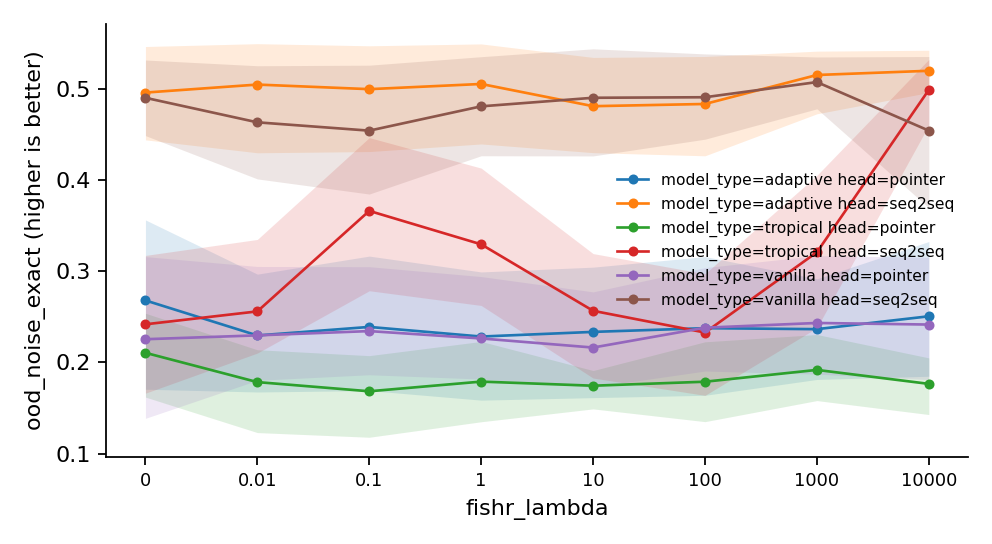
\includegraphics[width=\textwidth]{metric_ood_noise_exact.png}
\caption{\texttt{ood\_noise\_exact} against \texttt{fishr\_lambda}: the mean over seeds with a 95\% bootstrap CI, one line per combination of the other factors.}
\label{fig:ood_noise_exact}
\end{figure}

{\small
\begin{longtable}{lllrlrrr}
\caption{\texttt{ood\_noise\_exact} per cell: mean, 95\% bootstrap CI, SD, seeds, diverged runs.}\label{tab:summary-ood_noise_exact}\\
\toprule
\texttt{model\_type} & \texttt{head} & \texttt{fishr\_lambda} & mean & 95\% CI & SD & $n$ & div.\\
\midrule
\endhead
adaptive & pointer & 0 & 0.268 & [0.171, 0.356] & 0.12 & 5 & 0\\
adaptive & pointer & 0.01 & 0.2296 & [0.168, 0.297] & 0.0871 & 5 & 0\\
adaptive & pointer & 0.1 & 0.2389 & [0.169, 0.317] & 0.0952 & 5 & 0\\
adaptive & pointer & 1 & 0.2284 & [0.159, 0.299] & 0.0931 & 5 & 0\\
adaptive & pointer & 10 & 0.2335 & [0.161, 0.304] & 0.0895 & 5 & 0\\
adaptive & pointer & 100 & 0.2376 & [0.164, 0.316] & 0.0988 & 5 & 0\\
adaptive & pointer & 1000 & 0.2365 & [0.181, 0.292] & 0.0749 & 5 & 0\\
adaptive & pointer & 1e+04 & 0.2506 & [0.185, 0.333] & 0.0964 & 5 & 0\\
adaptive & seq2seq & 0 & 0.4957 & [0.444, 0.546] & 0.0645 & 5 & 0\\
adaptive & seq2seq & 0.01 & 0.5044 & [0.43, 0.549] & 0.0824 & 5 & 0\\
adaptive & seq2seq & 0.1 & 0.4994 & [0.431, 0.547] & 0.0823 & 5 & 0\\
adaptive & seq2seq & 1 & 0.5051 & [0.439, 0.549] & 0.073 & 5 & 0\\
adaptive & seq2seq & 10 & 0.4808 & [0.43, 0.534] & 0.0683 & 5 & 0\\
adaptive & seq2seq & 100 & 0.4832 & [0.426, 0.535] & 0.0764 & 5 & 0\\
adaptive & seq2seq & 1000 & 0.5149 & [0.472, 0.541] & 0.0475 & 5 & 0\\
adaptive & seq2seq & 1e+04 & 0.5195 & [0.496, 0.542] & 0.0298 & 5 & 0\\
tropical & pointer & 0 & 0.2106 & [0.162, 0.254] & 0.0589 & 5 & 0\\
tropical & pointer & 0.01 & 0.1785 & [0.123, 0.214] & 0.0577 & 5 & 0\\
tropical & pointer & 0.1 & 0.1684 & [0.118, 0.207] & 0.0576 & 5 & 0\\
tropical & pointer & 1 & 0.179 & [0.135, 0.223] & 0.0558 & 5 & 0\\
tropical & pointer & 10 & 0.1745 & [0.149, 0.191] & 0.0286 & 5 & 0\\
tropical & pointer & 100 & 0.1789 & [0.135, 0.223] & 0.0566 & 5 & 0\\
tropical & pointer & 1000 & 0.1919 & [0.158, 0.231] & 0.048 & 5 & 0\\
tropical & pointer & 1e+04 & 0.1766 & [0.143, 0.205] & 0.0404 & 5 & 0\\
tropical & seq2seq & 0 & 0.2418 & [0.166, 0.317] & 0.0974 & 5 & 0\\
tropical & seq2seq & 0.01 & 0.256 & [0.21, 0.335] & 0.0889 & 5 & 0\\
tropical & seq2seq & 0.1 & 0.3661 & [0.279, 0.446] & 0.104 & 5 & 0\\
tropical & seq2seq & 1 & 0.3294 & [0.262, 0.413] & 0.1 & 5 & 0\\
tropical & seq2seq & 10 & 0.2566 & [0.183, 0.319] & 0.0853 & 5 & 0\\
tropical & seq2seq & 100 & 0.2328 & [0.164, 0.297] & 0.0879 & 5 & 0\\
tropical & seq2seq & 1000 & 0.3208 & [0.238, 0.405] & 0.112 & 5 & 0\\
tropical & seq2seq & 1e+04 & 0.4987 & [0.46, 0.532] & 0.0455 & 5 & 0\\
vanilla & pointer & 0 & 0.2255 & [0.139, 0.316] & 0.117 & 5 & 0\\
vanilla & pointer & 0.01 & 0.2297 & [0.18, 0.305] & 0.0855 & 5 & 0\\
vanilla & pointer & 0.1 & 0.2344 & [0.187, 0.305] & 0.0803 & 5 & 0\\
vanilla & pointer & 1 & 0.2263 & [0.182, 0.294] & 0.0757 & 5 & 0\\
vanilla & pointer & 10 & 0.2163 & [0.173, 0.277] & 0.0673 & 5 & 0\\
vanilla & pointer & 100 & 0.2381 & [0.191, 0.304] & 0.0758 & 5 & 0\\
vanilla & pointer & 1000 & 0.2433 & [0.187, 0.317] & 0.0884 & 5 & 0\\
vanilla & pointer & 1e+04 & 0.2415 & [0.181, 0.315] & 0.0818 & 5 & 0\\
vanilla & seq2seq & 0 & 0.4899 & [0.449, 0.531] & 0.0525 & 5 & 0\\
vanilla & seq2seq & 0.01 & 0.4631 & [0.401, 0.525] & 0.0806 & 5 & 0\\
vanilla & seq2seq & 0.1 & 0.454 & [0.385, 0.526] & 0.0913 & 5 & 0\\
vanilla & seq2seq & 1 & 0.4806 & [0.426, 0.535] & 0.068 & 5 & 0\\
vanilla & seq2seq & 10 & 0.49 & [0.426, 0.544] & 0.075 & 5 & 0\\
vanilla & seq2seq & 100 & 0.4906 & [0.445, 0.538] & 0.06 & 5 & 0\\
vanilla & seq2seq & 1000 & 0.5072 & [0.478, 0.535] & 0.0409 & 5 & 0\\
vanilla & seq2seq & 1e+04 & 0.454 & [0.37, 0.535] & 0.109 & 5 & 0\\
\bottomrule
\end{longtable}
}

{\small
\begin{longtable}{lllrrrl}
\caption{\texttt{ood\_noise\_exact}: each level of \texttt{fishr\_lambda} against its control (0), within each combination of the other factors. parametric: Dunnett vs control.}\label{tab:control-ood_noise_exact}\\
\toprule
\texttt{model\_type} & \texttt{head} & \texttt{fishr\_lambda} & difference & 95\% CI & $p$ & \\
\midrule
\endhead
adaptive & pointer & 0.01 & -0.03838 & [-0.204, 0.128] & 0.9816 & \\
adaptive & pointer & 0.1 & -0.02904 & [-0.195, 0.137] & 0.9962 & \\
adaptive & pointer & 1 & -0.03958 & [-0.206, 0.126] & 0.9784 & \\
adaptive & pointer & 10 & -0.03448 & [-0.201, 0.132] & 0.9898 & \\
adaptive & pointer & 100 & -0.0304 & [-0.196, 0.136] & 0.9950 & \\
adaptive & pointer & 1000 & -0.03148 & [-0.198, 0.135] & 0.9939 & \\
adaptive & pointer & 1e+04 & -0.01738 & [-0.183, 0.149] & 0.9999 & \\
adaptive & seq2seq & 0.01 & 0.00876 & [-0.11, 0.127] & 1.0000 & \\
adaptive & seq2seq & 0.1 & 0.00374 & [-0.115, 0.122] & 1.0000 & \\
adaptive & seq2seq & 1 & 0.00942 & [-0.109, 0.128] & 1.0000 & \\
adaptive & seq2seq & 10 & -0.01492 & [-0.133, 0.103] & 0.9995 & \\
adaptive & seq2seq & 100 & -0.0125 & [-0.131, 0.106] & 0.9998 & \\
adaptive & seq2seq & 1000 & 0.01926 & [-0.099, 0.138] & 0.9975 & \\
adaptive & seq2seq & 1e+04 & 0.02386 & [-0.0944, 0.142] & 0.9913 & \\
tropical & pointer & 0.01 & -0.03208 & [-0.122, 0.0578] & 0.8622 & \\
tropical & pointer & 0.1 & -0.04214 & [-0.132, 0.0477] & 0.6625 & \\
tropical & pointer & 1 & -0.03154 & [-0.121, 0.0583] & 0.8710 & \\
tropical & pointer & 10 & -0.03604 & [-0.126, 0.0538] & 0.7903 & \\
tropical & pointer & 100 & -0.03166 & [-0.122, 0.0582] & 0.8690 & \\
tropical & pointer & 1000 & -0.01872 & [-0.109, 0.0712] & 0.9896 & \\
tropical & pointer & 1e+04 & -0.03402 & [-0.124, 0.0559] & 0.8286 & \\
tropical & seq2seq & 0.01 & 0.01414 & [-0.147, 0.175] & 1.0000 & \\
tropical & seq2seq & 0.1 & 0.1242 & [-0.0365, 0.285] & 0.1855 & \\
tropical & seq2seq & 1 & 0.0876 & [-0.0732, 0.248] & 0.5149 & \\
tropical & seq2seq & 10 & 0.01478 & [-0.146, 0.176] & 0.9999 & \\
tropical & seq2seq & 100 & -0.00902 & [-0.17, 0.152] & 1.0000 & \\
tropical & seq2seq & 1000 & 0.079 & [-0.0818, 0.24] & 0.6182 & \\
tropical & seq2seq & 1e+04 & 0.2568 & [0.0961, 0.418] & 0.0007 & *\\
vanilla & pointer & 0.01 & 0.00422 & [-0.144, 0.153] & 1.0000 & \\
vanilla & pointer & 0.1 & 0.0089 & [-0.14, 0.157] & 1.0000 & \\
vanilla & pointer & 1 & $8.400\times10^{-4}$ & [-0.148, 0.149] & 1.0000 & \\
vanilla & pointer & 10 & -0.00914 & [-0.158, 0.139] & 1.0000 & \\
vanilla & pointer & 100 & 0.0126 & [-0.136, 0.161] & 1.0000 & \\
vanilla & pointer & 1000 & 0.0178 & [-0.131, 0.166] & 0.9996 & \\
vanilla & pointer & 1e+04 & 0.01606 & [-0.133, 0.165] & 0.9998 & \\
vanilla & seq2seq & 0.01 & -0.02686 & [-0.158, 0.104] & 0.9905 & \\
vanilla & seq2seq & 0.1 & -0.03598 & [-0.167, 0.0951] & 0.9560 & \\
vanilla & seq2seq & 1 & -0.00934 & [-0.14, 0.122] & 1.0000 & \\
vanilla & seq2seq & 10 & $4.000\times10^{-5}$ & [-0.131, 0.131] & 1.0000 & \\
vanilla & seq2seq & 100 & $6.200\times10^{-4}$ & [-0.13, 0.132] & 1.0000 & \\
vanilla & seq2seq & 1000 & 0.01722 & [-0.114, 0.148] & 0.9994 & \\
vanilla & seq2seq & 1e+04 & -0.03596 & [-0.167, 0.0951] & 0.9561 & \\
\bottomrule
\end{longtable}
}

{\small
\begin{longtable}{llrrrrr}
\caption{\texttt{ood\_noise\_exact} against log10 \texttt{fishr\_lambda}: parametric: OLS slope t-test, seed-bootstrap CI, with the Jonckheere--Terpstra ordered-trend $\tau$ and $p$.}\label{tab:trend-ood_noise_exact}\\
\toprule
\texttt{model\_type} & \texttt{head} & estimate & 95\% CI & $p$ & JT $\tau$ & JT $p$\\
\midrule
\endhead
adaptive & pointer & 0.002404 & [-0.00321, 0.00597] & 0.7371 & 0.0876 & 0.5183\\
adaptive & seq2seq & 0.001944 & [-0.00705, 0.0151] & 0.7225 & -0.0571 & 0.6755\\
tropical & pointer & 0.001461 & [-0.00312, 0.00634] & 0.7138 & -0.0019 & 0.9910\\
tropical & seq2seq & 0.01932 & [0.00262, 0.0346] & 0.0535 & 0.272 & 0.0400\\
vanilla & pointer & 0.002324 & [$-6.16\times10^{-4}$, 0.00477] & 0.7112 & 0.0819 & 0.5495\\
vanilla & seq2seq & 0.003181 & [-0.00159, 0.00864] & 0.6142 & 0.0171 & 0.9102\\
\bottomrule
\end{longtable}
}

{\small
\begin{longtable}{lrrrl}
\caption{\texttt{ood\_noise\_exact}: paired contrasts by seed, Holm-corrected across the cells. parametric: paired t-test by seed, Holm.}\label{tab:paired-ood_noise_exact}\\
\toprule
contrast (within) & difference & 95\% CI & $p$ & \\
\midrule
\endhead
\stackcell{model\_type: tropical - vanilla\\\footnotesize head=pointer fishr\_lambda=0 } & -0.0149 & [-0.209, 0.179] & 1.0000 & \\
\stackcell{model\_type: tropical - vanilla\\\footnotesize head=pointer fishr\_lambda=0.01 } & -0.0512 & [-0.226, 0.124] & 1.0000 & \\
\stackcell{model\_type: tropical - vanilla\\\footnotesize head=pointer fishr\_lambda=0.1 } & -0.06594 & [-0.233, 0.101] & 1.0000 & \\
\stackcell{model\_type: tropical - vanilla\\\footnotesize head=pointer fishr\_lambda=1 } & -0.04728 & [-0.185, 0.0901] & 1.0000 & \\
\stackcell{model\_type: tropical - vanilla\\\footnotesize head=pointer fishr\_lambda=10 } & -0.0418 & [-0.16, 0.0765] & 1.0000 & \\
\stackcell{model\_type: tropical - vanilla\\\footnotesize head=pointer fishr\_lambda=100 } & -0.05916 & [-0.207, 0.089] & 1.0000 & \\
\stackcell{model\_type: tropical - vanilla\\\footnotesize head=pointer fishr\_lambda=1000 } & -0.05142 & [-0.185, 0.0817] & 1.0000 & \\
\stackcell{model\_type: tropical - vanilla\\\footnotesize head=pointer fishr\_lambda=1e+04 } & -0.06498 & [-0.213, 0.0831] & 1.0000 & \\
\stackcell{model\_type: tropical - vanilla\\\footnotesize head=seq2seq fishr\_lambda=0 } & -0.2481 & [-0.373, -0.124] & 0.0785 & \\
\stackcell{model\_type: tropical - vanilla\\\footnotesize head=seq2seq fishr\_lambda=0.01 } & -0.2071 & [-0.296, -0.118] & 0.0475 & *\\
\stackcell{model\_type: tropical - vanilla\\\footnotesize head=seq2seq fishr\_lambda=0.1 } & -0.0879 & [-0.187, 0.0115] & 0.7004 & \\
\stackcell{model\_type: tropical - vanilla\\\footnotesize head=seq2seq fishr\_lambda=1 } & -0.1512 & [-0.246, -0.0562] & 0.1496 & \\
\stackcell{model\_type: tropical - vanilla\\\footnotesize head=seq2seq fishr\_lambda=10 } & -0.2334 & [-0.386, -0.0811] & 0.1572 & \\
\stackcell{model\_type: tropical - vanilla\\\footnotesize head=seq2seq fishr\_lambda=100 } & -0.2578 & [-0.4, -0.115] & 0.1029 & \\
\stackcell{model\_type: tropical - vanilla\\\footnotesize head=seq2seq fishr\_lambda=1000 } & -0.1863 & [-0.371, -0.00171] & 0.5357 & \\
\stackcell{model\_type: tropical - vanilla\\\footnotesize head=seq2seq fishr\_lambda=1e+04 } & 0.04468 & [-0.0985, 0.188] & 1.0000 & \\
\stackcell{model\_type: adaptive - vanilla\\\footnotesize head=pointer fishr\_lambda=0 } & 0.0425 & [-0.089, 0.174] & 1.0000 & \\
\stackcell{model\_type: adaptive - vanilla\\\footnotesize head=pointer fishr\_lambda=0.01 } & $-1.000\times10^{-4}$ & [-0.0735, 0.0733] & 1.0000 & \\
\stackcell{model\_type: adaptive - vanilla\\\footnotesize head=pointer fishr\_lambda=0.1 } & 0.00456 & [-0.0644, 0.0735] & 1.0000 & \\
\stackcell{model\_type: adaptive - vanilla\\\footnotesize head=pointer fishr\_lambda=1 } & 0.00208 & [-0.0735, 0.0776] & 1.0000 & \\
\stackcell{model\_type: adaptive - vanilla\\\footnotesize head=pointer fishr\_lambda=10 } & 0.01716 & [-0.0709, 0.105] & 1.0000 & \\
\stackcell{model\_type: adaptive - vanilla\\\footnotesize head=pointer fishr\_lambda=100 } & $-5.000\times10^{-4}$ & [-0.0715, 0.0705] & 1.0000 & \\
\stackcell{model\_type: adaptive - vanilla\\\footnotesize head=pointer fishr\_lambda=1000 } & -0.00678 & [-0.0838, 0.0702] & 1.0000 & \\
\stackcell{model\_type: adaptive - vanilla\\\footnotesize head=pointer fishr\_lambda=1e+04 } & 0.00906 & [-0.0788, 0.0969] & 1.0000 & \\
\stackcell{model\_type: adaptive - vanilla\\\footnotesize head=seq2seq fishr\_lambda=0 } & 0.00574 & [-0.0512, 0.0627] & 1.0000 & \\
\stackcell{model\_type: adaptive - vanilla\\\footnotesize head=seq2seq fishr\_lambda=0.01 } & 0.04136 & [-0.0642, 0.147] & 1.0000 & \\
\stackcell{model\_type: adaptive - vanilla\\\footnotesize head=seq2seq fishr\_lambda=0.1 } & 0.04546 & [-0.0523, 0.143] & 1.0000 & \\
\stackcell{model\_type: adaptive - vanilla\\\footnotesize head=seq2seq fishr\_lambda=1 } & 0.0245 & [-0.0469, 0.0959] & 1.0000 & \\
\stackcell{model\_type: adaptive - vanilla\\\footnotesize head=seq2seq fishr\_lambda=10 } & -0.00922 & [-0.0675, 0.0491] & 1.0000 & \\
\stackcell{model\_type: adaptive - vanilla\\\footnotesize head=seq2seq fishr\_lambda=100 } & -0.00738 & [-0.0889, 0.0741] & 1.0000 & \\
\stackcell{model\_type: adaptive - vanilla\\\footnotesize head=seq2seq fishr\_lambda=1000 } & 0.00778 & [-0.0144, 0.03] & 1.0000 & \\
\stackcell{model\_type: adaptive - vanilla\\\footnotesize head=seq2seq fishr\_lambda=1e+04 } & 0.06556 & [-0.0339, 0.165] & 1.0000 & \\
\stackcell{head: pointer - seq2seq\\\footnotesize model\_type=adaptive fishr\_lambda=0 } & -0.2277 & [-0.373, -0.0822] & 0.0977 & \\
\stackcell{head: pointer - seq2seq\\\footnotesize model\_type=adaptive fishr\_lambda=0.01 } & -0.2748 & [-0.375, -0.175] & 0.0274 & *\\
\stackcell{head: pointer - seq2seq\\\footnotesize model\_type=adaptive fishr\_lambda=0.1 } & -0.2605 & [-0.358, -0.163] & 0.0274 & *\\
\stackcell{head: pointer - seq2seq\\\footnotesize model\_type=adaptive fishr\_lambda=1 } & -0.2767 & [-0.378, -0.176] & 0.0274 & *\\
\stackcell{head: pointer - seq2seq\\\footnotesize model\_type=adaptive fishr\_lambda=10 } & -0.2473 & [-0.307, -0.187] & 0.0080 & *\\
\stackcell{head: pointer - seq2seq\\\footnotesize model\_type=adaptive fishr\_lambda=100 } & -0.2456 & [-0.334, -0.157] & 0.0274 & *\\
\stackcell{head: pointer - seq2seq\\\footnotesize model\_type=adaptive fishr\_lambda=1000 } & -0.2784 & [-0.353, -0.204] & 0.0114 & *\\
\stackcell{head: pointer - seq2seq\\\footnotesize model\_type=adaptive fishr\_lambda=1e+04 } & -0.2689 & [-0.39, -0.148] & 0.0420 & *\\
\stackcell{head: pointer - seq2seq\\\footnotesize model\_type=tropical fishr\_lambda=0 } & -0.03124 & [-0.163, 0.101] & 0.5465 & \\
\stackcell{head: pointer - seq2seq\\\footnotesize model\_type=tropical fishr\_lambda=0.01 } & -0.07746 & [-0.186, 0.0315] & 0.4784 & \\
\stackcell{head: pointer - seq2seq\\\footnotesize model\_type=tropical fishr\_lambda=0.1 } & -0.1976 & [-0.369, -0.0259] & 0.2140 & \\
\stackcell{head: pointer - seq2seq\\\footnotesize model\_type=tropical fishr\_lambda=1 } & -0.1504 & [-0.318, 0.0174] & 0.3381 & \\
\stackcell{head: pointer - seq2seq\\\footnotesize model\_type=tropical fishr\_lambda=10 } & -0.08206 & [-0.215, 0.051] & 0.4859 & \\
\stackcell{head: pointer - seq2seq\\\footnotesize model\_type=tropical fishr\_lambda=100 } & -0.05388 & [-0.149, 0.0408] & 0.4859 & \\
\stackcell{head: pointer - seq2seq\\\footnotesize model\_type=tropical fishr\_lambda=1000 } & -0.129 & [-0.238, -0.0197] & 0.2140 & \\
\stackcell{head: pointer - seq2seq\\\footnotesize model\_type=tropical fishr\_lambda=1e+04 } & -0.3221 & [-0.414, -0.231] & 0.0136 & *\\
\stackcell{head: pointer - seq2seq\\\footnotesize model\_type=vanilla fishr\_lambda=0 } & -0.2645 & [-0.412, -0.117] & 0.0686 & \\
\stackcell{head: pointer - seq2seq\\\footnotesize model\_type=vanilla fishr\_lambda=0.01 } & -0.2334 & [-0.329, -0.137] & 0.0326 & *\\
\stackcell{head: pointer - seq2seq\\\footnotesize model\_type=vanilla fishr\_lambda=0.1 } & -0.2196 & [-0.322, -0.117] & 0.0438 & *\\
\stackcell{head: pointer - seq2seq\\\footnotesize model\_type=vanilla fishr\_lambda=1 } & -0.2543 & [-0.345, -0.164] & 0.0274 & *\\
\stackcell{head: pointer - seq2seq\\\footnotesize model\_type=vanilla fishr\_lambda=10 } & -0.2736 & [-0.36, -0.187] & 0.0194 & *\\
\stackcell{head: pointer - seq2seq\\\footnotesize model\_type=vanilla fishr\_lambda=100 } & -0.2525 & [-0.334, -0.171] & 0.0205 & *\\
\stackcell{head: pointer - seq2seq\\\footnotesize model\_type=vanilla fishr\_lambda=1000 } & -0.2639 & [-0.363, -0.165] & 0.0274 & *\\
\stackcell{head: pointer - seq2seq\\\footnotesize model\_type=vanilla fishr\_lambda=1e+04 } & -0.2124 & [-0.32, -0.105] & 0.0530 & \\
\bottomrule
\end{longtable}
}

\subsection{\texttt{id\_f1}}
\begin{figure}[tbp]
\centering
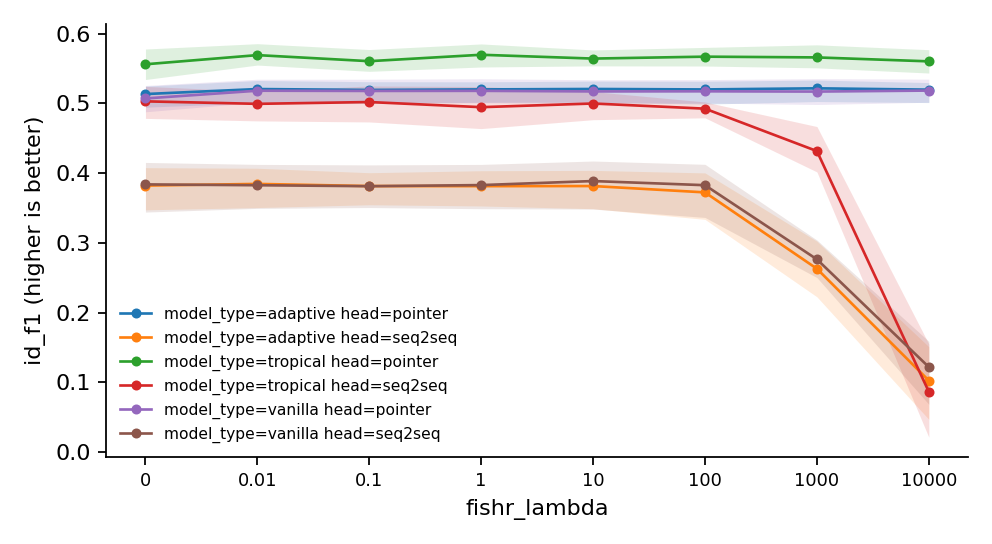
\includegraphics[width=\textwidth]{metric_id_f1.png}
\caption{\texttt{id\_f1} against \texttt{fishr\_lambda}: the mean over seeds with a 95\% bootstrap CI, one line per combination of the other factors.}
\label{fig:id_f1}
\end{figure}

{\small
\begin{longtable}{lllrlrrr}
\caption{\texttt{id\_f1} per cell: mean, 95\% bootstrap CI, SD, seeds, diverged runs.}\label{tab:summary-id_f1}\\
\toprule
\texttt{model\_type} & \texttt{head} & \texttt{fishr\_lambda} & mean & 95\% CI & SD & $n$ & div.\\
\midrule
\endhead
adaptive & pointer & 0 & 0.5135 & [0.495, 0.525] & 0.0211 & 5 & 0\\
adaptive & pointer & 0.01 & 0.5207 & [0.501, 0.533] & 0.0221 & 5 & 0\\
adaptive & pointer & 0.1 & 0.5195 & [0.5, 0.531] & 0.0214 & 5 & 0\\
adaptive & pointer & 1 & 0.5202 & [0.502, 0.531] & 0.0208 & 5 & 0\\
adaptive & pointer & 10 & 0.5208 & [0.502, 0.532] & 0.0213 & 5 & 0\\
adaptive & pointer & 100 & 0.5202 & [0.499, 0.532] & 0.0232 & 5 & 0\\
adaptive & pointer & 1000 & 0.5218 & [0.503, 0.534] & 0.0211 & 5 & 0\\
adaptive & pointer & 1e+04 & 0.5199 & [0.501, 0.53] & 0.0205 & 5 & 0\\
adaptive & seq2seq & 0 & 0.3822 & [0.347, 0.408] & 0.0401 & 5 & 0\\
adaptive & seq2seq & 0.01 & 0.3846 & [0.351, 0.407] & 0.0377 & 5 & 0\\
adaptive & seq2seq & 0.1 & 0.3815 & [0.355, 0.401] & 0.0309 & 5 & 0\\
adaptive & seq2seq & 1 & 0.3814 & [0.353, 0.404] & 0.0337 & 5 & 0\\
adaptive & seq2seq & 10 & 0.3815 & [0.349, 0.404] & 0.0369 & 5 & 0\\
adaptive & seq2seq & 100 & 0.3724 & [0.334, 0.4] & 0.0442 & 5 & 0\\
adaptive & seq2seq & 1000 & 0.2629 & [0.223, 0.302] & 0.0522 & 5 & 0\\
adaptive & seq2seq & 1e+04 & 0.1024 & [0.0467, 0.151] & 0.067 & 5 & 0\\
tropical & pointer & 0 & 0.5563 & [0.534, 0.578] & 0.0277 & 5 & 0\\
tropical & pointer & 0.01 & 0.5694 & [0.555, 0.586] & 0.0199 & 5 & 0\\
tropical & pointer & 0.1 & 0.5607 & [0.546, 0.577] & 0.0211 & 5 & 0\\
tropical & pointer & 1 & 0.5699 & [0.552, 0.585] & 0.022 & 5 & 0\\
tropical & pointer & 10 & 0.5644 & [0.554, 0.577] & 0.0146 & 5 & 0\\
tropical & pointer & 100 & 0.5672 & [0.554, 0.58] & 0.0179 & 5 & 0\\
tropical & pointer & 1000 & 0.5661 & [0.551, 0.584] & 0.0216 & 5 & 0\\
tropical & pointer & 1e+04 & 0.5604 & [0.544, 0.577] & 0.0219 & 5 & 0\\
tropical & seq2seq & 0 & 0.5031 & [0.479, 0.525] & 0.0296 & 5 & 0\\
tropical & seq2seq & 0.01 & 0.4995 & [0.475, 0.518] & 0.0289 & 5 & 0\\
tropical & seq2seq & 0.1 & 0.5021 & [0.473, 0.525] & 0.0341 & 5 & 0\\
tropical & seq2seq & 1 & 0.4947 & [0.464, 0.524] & 0.0367 & 5 & 0\\
tropical & seq2seq & 10 & 0.5 & [0.477, 0.517] & 0.0255 & 5 & 0\\
tropical & seq2seq & 100 & 0.4926 & [0.479, 0.502] & 0.0159 & 5 & 0\\
tropical & seq2seq & 1000 & 0.4317 & [0.402, 0.467] & 0.0409 & 5 & 0\\
tropical & seq2seq & 1e+04 & 0.0864 & [0.0211, 0.155] & 0.0855 & 5 & 0\\
vanilla & pointer & 0 & 0.5072 & [0.488, 0.526] & 0.0252 & 5 & 0\\
vanilla & pointer & 0.01 & 0.5183 & [0.502, 0.535] & 0.0218 & 5 & 0\\
vanilla & pointer & 0.1 & 0.518 & [0.501, 0.535] & 0.022 & 5 & 0\\
vanilla & pointer & 1 & 0.5182 & [0.501, 0.535] & 0.0226 & 5 & 0\\
vanilla & pointer & 10 & 0.5173 & [0.501, 0.534] & 0.0224 & 5 & 0\\
vanilla & pointer & 100 & 0.5175 & [0.501, 0.534] & 0.0221 & 5 & 0\\
vanilla & pointer & 1000 & 0.5171 & [0.499, 0.536] & 0.0248 & 5 & 0\\
vanilla & pointer & 1e+04 & 0.5185 & [0.502, 0.535] & 0.0222 & 5 & 0\\
vanilla & seq2seq & 0 & 0.3839 & [0.344, 0.415] & 0.0467 & 5 & 0\\
vanilla & seq2seq & 0.01 & 0.3827 & [0.349, 0.413] & 0.0409 & 5 & 0\\
vanilla & seq2seq & 0.1 & 0.3813 & [0.351, 0.412] & 0.0423 & 5 & 0\\
vanilla & seq2seq & 1 & 0.3829 & [0.349, 0.413] & 0.0404 & 5 & 0\\
vanilla & seq2seq & 10 & 0.3887 & [0.349, 0.417] & 0.0461 & 5 & 0\\
vanilla & seq2seq & 100 & 0.3828 & [0.336, 0.413] & 0.0505 & 5 & 0\\
vanilla & seq2seq & 1000 & 0.2764 & [0.25, 0.304] & 0.0336 & 5 & 0\\
vanilla & seq2seq & 1e+04 & 0.1218 & [0.0684, 0.159] & 0.0591 & 5 & 0\\
\bottomrule
\end{longtable}
}

{\small
\begin{longtable}{lllrrrl}
\caption{\texttt{id\_f1}: each level of \texttt{fishr\_lambda} against its control (0), within each combination of the other factors. parametric: Dunnett vs control.}\label{tab:control-id_f1}\\
\toprule
\texttt{model\_type} & \texttt{head} & \texttt{fishr\_lambda} & difference & 95\% CI & $p$ & \\
\midrule
\endhead
adaptive & pointer & 0.01 & 0.007179 & [-0.0303, 0.0447] & 0.9936 & \\
adaptive & pointer & 0.1 & 0.00593 & [-0.0316, 0.0434] & 0.9979 & \\
adaptive & pointer & 1 & 0.006643 & [-0.0308, 0.0441] & 0.9959 & \\
adaptive & pointer & 10 & 0.007283 & [-0.0302, 0.0448] & 0.9930 & \\
adaptive & pointer & 100 & 0.006625 & [-0.0309, 0.0441] & 0.9960 & \\
adaptive & pointer & 1000 & 0.008216 & [-0.0293, 0.0457] & 0.9862 & \\
adaptive & pointer & 1e+04 & 0.006318 & [-0.0312, 0.0438] & 0.9970 & \\
adaptive & seq2seq & 0.01 & 0.002401 & [-0.0749, 0.0797] & 1.0000 & \\
adaptive & seq2seq & 0.1 & $-6.942\times10^{-4}$ & [-0.0779, 0.0766] & 1.0000 & \\
adaptive & seq2seq & 1 & $-8.149\times10^{-4}$ & [-0.0781, 0.0764] & 1.0000 & \\
adaptive & seq2seq & 10 & $-6.654\times10^{-4}$ & [-0.0779, 0.0766] & 1.0000 & \\
adaptive & seq2seq & 100 & -0.00976 & [-0.087, 0.0675] & 0.9995 & \\
adaptive & seq2seq & 1000 & -0.1193 & [-0.197, -0.0421] & 0.0010 & *\\
adaptive & seq2seq & 1e+04 & -0.2798 & [-0.357, -0.203] & $<10^{-4}$ & *\\
tropical & pointer & 0.01 & 0.01314 & [-0.0238, 0.0501] & 0.8635 & \\
tropical & pointer & 0.1 & 0.004439 & [-0.0325, 0.0414] & 0.9996 & \\
tropical & pointer & 1 & 0.01364 & [-0.0233, 0.0506] & 0.8430 & \\
tropical & pointer & 10 & 0.008164 & [-0.0288, 0.0451] & 0.9855 & \\
tropical & pointer & 100 & 0.01093 & [-0.026, 0.0478] & 0.9372 & \\
tropical & pointer & 1000 & 0.009839 & [-0.0271, 0.0468] & 0.9618 & \\
tropical & pointer & 1e+04 & 0.004186 & [-0.0327, 0.0411] & 0.9998 & \\
tropical & seq2seq & 0.01 & -0.003576 & [-0.0769, 0.0698] & 1.0000 & \\
tropical & seq2seq & 0.1 & $-9.973\times10^{-4}$ & [-0.0743, 0.0724] & 1.0000 & \\
tropical & seq2seq & 1 & -0.008355 & [-0.0817, 0.065] & 0.9997 & \\
tropical & seq2seq & 10 & -0.003091 & [-0.0764, 0.0703] & 1.0000 & \\
tropical & seq2seq & 100 & -0.01049 & [-0.0838, 0.0629] & 0.9989 & \\
tropical & seq2seq & 1000 & -0.07138 & [-0.145, 0.00197] & 0.0591 & \\
tropical & seq2seq & 1e+04 & -0.4167 & [-0.49, -0.343] & $<10^{-4}$ & *\\
vanilla & pointer & 0.01 & 0.01113 & [-0.0289, 0.0512] & 0.9533 & \\
vanilla & pointer & 0.1 & 0.01079 & [-0.0293, 0.0508] & 0.9600 & \\
vanilla & pointer & 1 & 0.01094 & [-0.0291, 0.051] & 0.9570 & \\
vanilla & pointer & 10 & 0.01008 & [-0.03, 0.0501] & 0.9714 & \\
vanilla & pointer & 100 & 0.01024 & [-0.0298, 0.0503] & 0.9690 & \\
vanilla & pointer & 1000 & 0.009875 & [-0.0302, 0.0499] & 0.9742 & \\
vanilla & pointer & 1e+04 & 0.01131 & [-0.0288, 0.0514] & 0.9498 & \\
vanilla & seq2seq & 0.01 & -0.001203 & [-0.0807, 0.0783] & 1.0000 & \\
vanilla & seq2seq & 0.1 & -0.002582 & [-0.0821, 0.0769] & 1.0000 & \\
vanilla & seq2seq & 1 & -0.001009 & [-0.0805, 0.0785] & 1.0000 & \\
vanilla & seq2seq & 10 & 0.004793 & [-0.0747, 0.0843] & 1.0000 & \\
vanilla & seq2seq & 100 & -0.001145 & [-0.0806, 0.0783] & 1.0000 & \\
vanilla & seq2seq & 1000 & -0.1075 & [-0.187, -0.028] & 0.0044 & *\\
vanilla & seq2seq & 1e+04 & -0.2621 & [-0.342, -0.183] & $<10^{-4}$ & *\\
\bottomrule
\end{longtable}
}

{\small
\begin{longtable}{llrrrrr}
\caption{\texttt{id\_f1} against log10 \texttt{fishr\_lambda}: parametric: OLS slope t-test, seed-bootstrap CI, with the Jonckheere--Terpstra ordered-trend $\tau$ and $p$.}\label{tab:trend-id_f1}\\
\toprule
\texttt{model\_type} & \texttt{head} & estimate & 95\% CI & $p$ & JT $\tau$ & JT $p$\\
\midrule
\endhead
adaptive & pointer & $7.045\times10^{-5}$ & [$-1.74\times10^{-4}$, $3.59\times10^{-4}$] & 0.9667 & 0.00952 & 0.9544\\
adaptive & seq2seq & -0.03903 & [-0.0429, -0.0346] & $<10^{-4}$ & -0.558 & 0.0002\\
tropical & pointer & $-6.706\times10^{-4}$ & [-0.00171, $3.73\times10^{-4}$] & 0.6748 & -0.0362 & 0.7938\\
tropical & seq2seq & -0.04936 & [-0.0575, -0.0402] & $<10^{-4}$ & -0.558 & 0.0002\\
vanilla & pointer & $-7.105\times10^{-5}$ & [$-3.49\times10^{-4}$, $2.07\times10^{-4}$] & 0.9680 & -0.00952 & 0.9556\\
vanilla & seq2seq & -0.03545 & [-0.0405, -0.0299] & $<10^{-4}$ & -0.493 & 0.0002\\
\bottomrule
\end{longtable}
}

{\small
\begin{longtable}{lrrrl}
\caption{\texttt{id\_f1}: paired contrasts by seed, Holm-corrected across the cells. parametric: paired t-test by seed, Holm.}\label{tab:paired-id_f1}\\
\toprule
contrast (within) & difference & 95\% CI & $p$ & \\
\midrule
\endhead
\stackcell{model\_type: tropical - vanilla\\\footnotesize head=pointer fishr\_lambda=0 } & 0.04904 & [$-5.79\times10^{-4}$, 0.0987] & 0.1655 & \\
\stackcell{model\_type: tropical - vanilla\\\footnotesize head=pointer fishr\_lambda=0.01 } & 0.05106 & [0.0128, 0.0893] & 0.1393 & \\
\stackcell{model\_type: tropical - vanilla\\\footnotesize head=pointer fishr\_lambda=0.1 } & 0.0427 & [0.00181, 0.0836] & 0.1655 & \\
\stackcell{model\_type: tropical - vanilla\\\footnotesize head=pointer fishr\_lambda=1 } & 0.05174 & [0.0146, 0.0889] & 0.1393 & \\
\stackcell{model\_type: tropical - vanilla\\\footnotesize head=pointer fishr\_lambda=10 } & 0.04713 & [0.0146, 0.0796] & 0.1393 & \\
\stackcell{model\_type: tropical - vanilla\\\footnotesize head=pointer fishr\_lambda=100 } & 0.04973 & [0.0156, 0.0838] & 0.1393 & \\
\stackcell{model\_type: tropical - vanilla\\\footnotesize head=pointer fishr\_lambda=1000 } & 0.04901 & [0.00311, 0.0949] & 0.1655 & \\
\stackcell{model\_type: tropical - vanilla\\\footnotesize head=pointer fishr\_lambda=1e+04 } & 0.04192 & [0.0105, 0.0734] & 0.1393 & \\
\stackcell{model\_type: tropical - vanilla\\\footnotesize head=seq2seq fishr\_lambda=0 } & 0.1192 & [0.0652, 0.173] & 0.0358 & *\\
\stackcell{model\_type: tropical - vanilla\\\footnotesize head=seq2seq fishr\_lambda=0.01 } & 0.1168 & [0.0741, 0.159] & 0.0225 & *\\
\stackcell{model\_type: tropical - vanilla\\\footnotesize head=seq2seq fishr\_lambda=0.1 } & 0.1207 & [0.0753, 0.166] & 0.0235 & *\\
\stackcell{model\_type: tropical - vanilla\\\footnotesize head=seq2seq fishr\_lambda=1 } & 0.1118 & [0.0649, 0.159] & 0.0324 & *\\
\stackcell{model\_type: tropical - vanilla\\\footnotesize head=seq2seq fishr\_lambda=10 } & 0.1113 & [0.0747, 0.148] & 0.0162 & *\\
\stackcell{model\_type: tropical - vanilla\\\footnotesize head=seq2seq fishr\_lambda=100 } & 0.1098 & [0.063, 0.157] & 0.0324 & *\\
\stackcell{model\_type: tropical - vanilla\\\footnotesize head=seq2seq fishr\_lambda=1000 } & 0.1553 & [0.119, 0.191] & 0.0045 & *\\
\stackcell{model\_type: tropical - vanilla\\\footnotesize head=seq2seq fishr\_lambda=1e+04 } & -0.03542 & [-0.135, 0.0643] & 0.3797 & \\
\stackcell{model\_type: adaptive - vanilla\\\footnotesize head=pointer fishr\_lambda=0 } & 0.006318 & [-0.0132, 0.0258] & 1.0000 & \\
\stackcell{model\_type: adaptive - vanilla\\\footnotesize head=pointer fishr\_lambda=0.01 } & 0.002366 & [-0.0225, 0.0272] & 1.0000 & \\
\stackcell{model\_type: adaptive - vanilla\\\footnotesize head=pointer fishr\_lambda=0.1 } & 0.001463 & [-0.0222, 0.0252] & 1.0000 & \\
\stackcell{model\_type: adaptive - vanilla\\\footnotesize head=pointer fishr\_lambda=1 } & 0.002021 & [-0.0211, 0.0251] & 1.0000 & \\
\stackcell{model\_type: adaptive - vanilla\\\footnotesize head=pointer fishr\_lambda=10 } & 0.00352 & [-0.0208, 0.0278] & 1.0000 & \\
\stackcell{model\_type: adaptive - vanilla\\\footnotesize head=pointer fishr\_lambda=100 } & 0.0027 & [-0.0211, 0.0265] & 1.0000 & \\
\stackcell{model\_type: adaptive - vanilla\\\footnotesize head=pointer fishr\_lambda=1000 } & 0.004659 & [-0.0178, 0.0271] & 1.0000 & \\
\stackcell{model\_type: adaptive - vanilla\\\footnotesize head=pointer fishr\_lambda=1e+04 } & 0.00133 & [-0.0227, 0.0254] & 1.0000 & \\
\stackcell{model\_type: adaptive - vanilla\\\footnotesize head=seq2seq fishr\_lambda=0 } & -0.001708 & [-0.0304, 0.027] & 1.0000 & \\
\stackcell{model\_type: adaptive - vanilla\\\footnotesize head=seq2seq fishr\_lambda=0.01 } & 0.001896 & [-0.0212, 0.025] & 1.0000 & \\
\stackcell{model\_type: adaptive - vanilla\\\footnotesize head=seq2seq fishr\_lambda=0.1 } & $1.799\times10^{-4}$ & [-0.0186, 0.019] & 1.0000 & \\
\stackcell{model\_type: adaptive - vanilla\\\footnotesize head=seq2seq fishr\_lambda=1 } & -0.001514 & [-0.0176, 0.0146] & 1.0000 & \\
\stackcell{model\_type: adaptive - vanilla\\\footnotesize head=seq2seq fishr\_lambda=10 } & -0.007167 & [-0.0263, 0.012] & 1.0000 & \\
\stackcell{model\_type: adaptive - vanilla\\\footnotesize head=seq2seq fishr\_lambda=100 } & -0.01032 & [-0.0431, 0.0225] & 1.0000 & \\
\stackcell{model\_type: adaptive - vanilla\\\footnotesize head=seq2seq fishr\_lambda=1000 } & -0.01348 & [-0.0437, 0.0167] & 1.0000 & \\
\stackcell{model\_type: adaptive - vanilla\\\footnotesize head=seq2seq fishr\_lambda=1e+04 } & -0.0194 & [-0.0519, 0.0131] & 1.0000 & \\
\stackcell{head: pointer - seq2seq\\\footnotesize model\_type=adaptive fishr\_lambda=0 } & 0.1313 & [0.074, 0.189] & 0.0294 & *\\
\stackcell{head: pointer - seq2seq\\\footnotesize model\_type=adaptive fishr\_lambda=0.01 } & 0.1361 & [0.0792, 0.193] & 0.0294 & *\\
\stackcell{head: pointer - seq2seq\\\footnotesize model\_type=adaptive fishr\_lambda=0.1 } & 0.138 & [0.0907, 0.185] & 0.0240 & *\\
\stackcell{head: pointer - seq2seq\\\footnotesize model\_type=adaptive fishr\_lambda=1 } & 0.1388 & [0.088, 0.19] & 0.0281 & *\\
\stackcell{head: pointer - seq2seq\\\footnotesize model\_type=adaptive fishr\_lambda=10 } & 0.1393 & [0.0839, 0.195] & 0.0292 & *\\
\stackcell{head: pointer - seq2seq\\\footnotesize model\_type=adaptive fishr\_lambda=100 } & 0.1477 & [0.0849, 0.211] & 0.0294 & *\\
\stackcell{head: pointer - seq2seq\\\footnotesize model\_type=adaptive fishr\_lambda=1000 } & 0.2589 & [0.176, 0.341] & 0.0190 & *\\
\stackcell{head: pointer - seq2seq\\\footnotesize model\_type=adaptive fishr\_lambda=1e+04 } & 0.4174 & [0.32, 0.515] & 0.0064 & *\\
\stackcell{head: pointer - seq2seq\\\footnotesize model\_type=tropical fishr\_lambda=0 } & 0.0532 & [0.0192, 0.0872] & 0.0438 & *\\
\stackcell{head: pointer - seq2seq\\\footnotesize model\_type=tropical fishr\_lambda=0.01 } & 0.06991 & [0.0297, 0.11] & 0.0438 & *\\
\stackcell{head: pointer - seq2seq\\\footnotesize model\_type=tropical fishr\_lambda=0.1 } & 0.05863 & [0.00974, 0.108] & 0.0513 & \\
\stackcell{head: pointer - seq2seq\\\footnotesize model\_type=tropical fishr\_lambda=1 } & 0.07519 & [0.015, 0.135] & 0.0513 & \\
\stackcell{head: pointer - seq2seq\\\footnotesize model\_type=tropical fishr\_lambda=10 } & 0.06445 & [0.0333, 0.0956] & 0.0365 & *\\
\stackcell{head: pointer - seq2seq\\\footnotesize model\_type=tropical fishr\_lambda=100 } & 0.07461 & [0.0476, 0.102] & 0.0281 & *\\
\stackcell{head: pointer - seq2seq\\\footnotesize model\_type=tropical fishr\_lambda=1000 } & 0.1344 & [0.0819, 0.187] & 0.0292 & *\\
\stackcell{head: pointer - seq2seq\\\footnotesize model\_type=tropical fishr\_lambda=1e+04 } & 0.474 & [0.359, 0.589] & 0.0069 & *\\
\stackcell{head: pointer - seq2seq\\\footnotesize model\_type=vanilla fishr\_lambda=0 } & 0.1233 & [0.0553, 0.191] & 0.0438 & *\\
\stackcell{head: pointer - seq2seq\\\footnotesize model\_type=vanilla fishr\_lambda=0.01 } & 0.1356 & [0.0859, 0.185] & 0.0281 & *\\
\stackcell{head: pointer - seq2seq\\\footnotesize model\_type=vanilla fishr\_lambda=0.1 } & 0.1367 & [0.0823, 0.191] & 0.0292 & *\\
\stackcell{head: pointer - seq2seq\\\footnotesize model\_type=vanilla fishr\_lambda=1 } & 0.1353 & [0.0833, 0.187] & 0.0292 & *\\
\stackcell{head: pointer - seq2seq\\\footnotesize model\_type=vanilla fishr\_lambda=10 } & 0.1286 & [0.0644, 0.193] & 0.0365 & *\\
\stackcell{head: pointer - seq2seq\\\footnotesize model\_type=vanilla fishr\_lambda=100 } & 0.1347 & [0.0561, 0.213] & 0.0438 & *\\
\stackcell{head: pointer - seq2seq\\\footnotesize model\_type=vanilla fishr\_lambda=1000 } & 0.2407 & [0.189, 0.293] & 0.0051 & *\\
\stackcell{head: pointer - seq2seq\\\footnotesize model\_type=vanilla fishr\_lambda=1e+04 } & 0.3967 & [0.308, 0.485] & 0.0055 & *\\
\bottomrule
\end{longtable}
}

\subsection{\texttt{id\_exact}}
\begin{figure}[tbp]
\centering
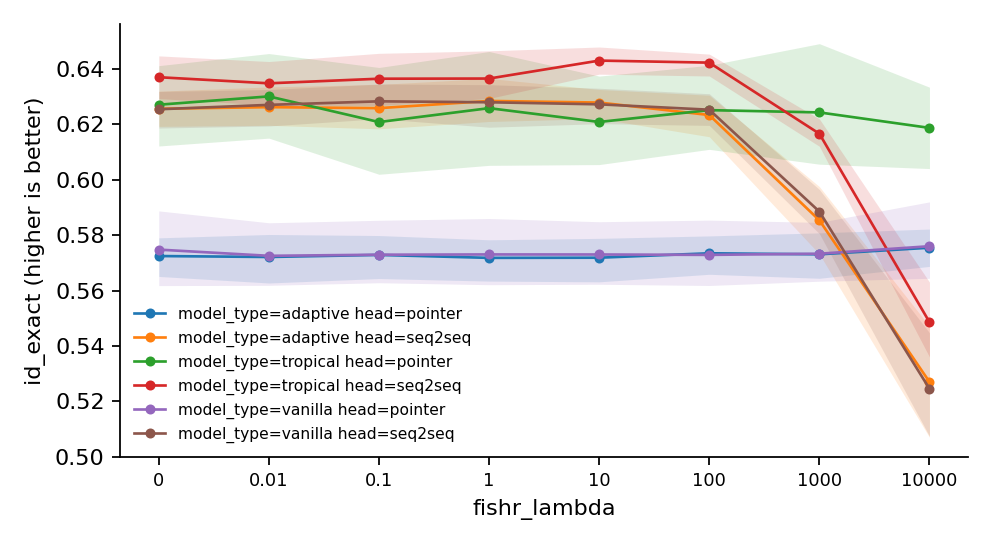
\includegraphics[width=\textwidth]{metric_id_exact.png}
\caption{\texttt{id\_exact} against \texttt{fishr\_lambda}: the mean over seeds with a 95\% bootstrap CI, one line per combination of the other factors.}
\label{fig:id_exact}
\end{figure}

{\small
\begin{longtable}{lllrlrrr}
\caption{\texttt{id\_exact} per cell: mean, 95\% bootstrap CI, SD, seeds, diverged runs.}\label{tab:summary-id_exact}\\
\toprule
\texttt{model\_type} & \texttt{head} & \texttt{fishr\_lambda} & mean & 95\% CI & SD & $n$ & div.\\
\midrule
\endhead
adaptive & pointer & 0 & 0.5724 & [0.565, 0.579] & 0.00944 & 5 & 0\\
adaptive & pointer & 0.01 & 0.5721 & [0.563, 0.58] & 0.0111 & 5 & 0\\
adaptive & pointer & 0.1 & 0.5728 & [0.564, 0.58] & 0.00986 & 5 & 0\\
adaptive & pointer & 1 & 0.5718 & [0.563, 0.578] & 0.00975 & 5 & 0\\
adaptive & pointer & 10 & 0.5718 & [0.563, 0.579] & 0.0102 & 5 & 0\\
adaptive & pointer & 100 & 0.5734 & [0.566, 0.58] & 0.00894 & 5 & 0\\
adaptive & pointer & 1000 & 0.5731 & [0.564, 0.581] & 0.00999 & 5 & 0\\
adaptive & pointer & 1e+04 & 0.5754 & [0.569, 0.582] & 0.00901 & 5 & 0\\
adaptive & seq2seq & 0 & 0.6256 & [0.619, 0.632] & 0.00769 & 5 & 0\\
adaptive & seq2seq & 0.01 & 0.6262 & [0.62, 0.633] & 0.00881 & 5 & 0\\
adaptive & seq2seq & 0.1 & 0.6258 & [0.618, 0.634] & 0.00997 & 5 & 0\\
adaptive & seq2seq & 1 & 0.6284 & [0.621, 0.637] & 0.00987 & 5 & 0\\
adaptive & seq2seq & 10 & 0.6278 & [0.622, 0.633] & 0.00677 & 5 & 0\\
adaptive & seq2seq & 100 & 0.6233 & [0.615, 0.63] & 0.00972 & 5 & 0\\
adaptive & seq2seq & 1000 & 0.5853 & [0.573, 0.598] & 0.0166 & 5 & 0\\
adaptive & seq2seq & 1e+04 & 0.527 & [0.507, 0.547] & 0.0275 & 5 & 0\\
tropical & pointer & 0 & 0.627 & [0.612, 0.641] & 0.0186 & 5 & 0\\
tropical & pointer & 0.01 & 0.63 & [0.615, 0.645] & 0.0197 & 5 & 0\\
tropical & pointer & 0.1 & 0.6208 & [0.602, 0.64] & 0.0262 & 5 & 0\\
tropical & pointer & 1 & 0.6258 & [0.605, 0.646] & 0.0277 & 5 & 0\\
tropical & pointer & 10 & 0.6208 & [0.605, 0.637] & 0.0205 & 5 & 0\\
tropical & pointer & 100 & 0.6251 & [0.611, 0.641] & 0.0191 & 5 & 0\\
tropical & pointer & 1000 & 0.6243 & [0.606, 0.649] & 0.0266 & 5 & 0\\
tropical & pointer & 1e+04 & 0.6187 & [0.604, 0.633] & 0.0184 & 5 & 0\\
tropical & seq2seq & 0 & 0.637 & [0.629, 0.645] & 0.01 & 5 & 0\\
tropical & seq2seq & 0.01 & 0.6348 & [0.627, 0.643] & 0.0101 & 5 & 0\\
tropical & seq2seq & 0.1 & 0.6364 & [0.627, 0.646] & 0.0123 & 5 & 0\\
tropical & seq2seq & 1 & 0.6365 & [0.629, 0.646] & 0.0112 & 5 & 0\\
tropical & seq2seq & 10 & 0.643 & [0.638, 0.648] & 0.0064 & 5 & 0\\
tropical & seq2seq & 100 & 0.6422 & [0.637, 0.645] & 0.00548 & 5 & 0\\
tropical & seq2seq & 1000 & 0.6166 & [0.612, 0.622] & 0.00649 & 5 & 0\\
tropical & seq2seq & 1e+04 & 0.5486 & [0.536, 0.563] & 0.0183 & 5 & 0\\
vanilla & pointer & 0 & 0.5748 & [0.562, 0.589] & 0.0169 & 5 & 0\\
vanilla & pointer & 0.01 & 0.5725 & [0.562, 0.584] & 0.0147 & 5 & 0\\
vanilla & pointer & 0.1 & 0.5729 & [0.563, 0.585] & 0.0154 & 5 & 0\\
vanilla & pointer & 1 & 0.573 & [0.562, 0.586] & 0.0154 & 5 & 0\\
vanilla & pointer & 10 & 0.573 & [0.562, 0.585] & 0.015 & 5 & 0\\
vanilla & pointer & 100 & 0.5729 & [0.562, 0.585] & 0.0151 & 5 & 0\\
vanilla & pointer & 1000 & 0.5733 & [0.563, 0.585] & 0.0143 & 5 & 0\\
vanilla & pointer & 1e+04 & 0.576 & [0.564, 0.592] & 0.0186 & 5 & 0\\
vanilla & seq2seq & 0 & 0.6254 & [0.619, 0.632] & 0.0079 & 5 & 0\\
vanilla & seq2seq & 0.01 & 0.627 & [0.619, 0.633] & 0.00859 & 5 & 0\\
vanilla & seq2seq & 0.1 & 0.6283 & [0.622, 0.635] & 0.00767 & 5 & 0\\
vanilla & seq2seq & 1 & 0.6279 & [0.619, 0.634] & 0.0097 & 5 & 0\\
vanilla & seq2seq & 10 & 0.6272 & [0.62, 0.633] & 0.00843 & 5 & 0\\
vanilla & seq2seq & 100 & 0.6252 & [0.62, 0.631] & 0.00726 & 5 & 0\\
vanilla & seq2seq & 1000 & 0.5885 & [0.581, 0.596] & 0.0106 & 5 & 0\\
vanilla & seq2seq & 1e+04 & 0.5246 & [0.507, 0.545] & 0.0241 & 5 & 0\\
\bottomrule
\end{longtable}
}

{\small
\begin{longtable}{lllrrrl}
\caption{\texttt{id\_exact}: each level of \texttt{fishr\_lambda} against its control (0), within each combination of the other factors. parametric: Dunnett vs control.}\label{tab:control-id_exact}\\
\toprule
\texttt{model\_type} & \texttt{head} & \texttt{fishr\_lambda} & difference & 95\% CI & $p$ & \\
\midrule
\endhead
adaptive & pointer & 0.01 & $-3.400\times10^{-4}$ & [-0.0175, 0.0168] & 1.0000 & \\
adaptive & pointer & 0.1 & $4.000\times10^{-4}$ & [-0.0167, 0.0175] & 1.0000 & \\
adaptive & pointer & 1 & $-6.600\times10^{-4}$ & [-0.0178, 0.0165] & 1.0000 & \\
adaptive & pointer & 10 & $-6.000\times10^{-4}$ & [-0.0177, 0.0165] & 1.0000 & \\
adaptive & pointer & 100 & 0.001 & [-0.0161, 0.0181] & 1.0000 & \\
adaptive & pointer & 1000 & $6.200\times10^{-4}$ & [-0.0165, 0.0177] & 1.0000 & \\
adaptive & pointer & 1e+04 & 0.003 & [-0.0141, 0.0201] & 0.9962 & \\
adaptive & seq2seq & 0.01 & $5.800\times10^{-4}$ & [-0.0234, 0.0245] & 1.0000 & \\
adaptive & seq2seq & 0.1 & $2.200\times10^{-4}$ & [-0.0237, 0.0242] & 1.0000 & \\
adaptive & seq2seq & 1 & 0.00282 & [-0.0211, 0.0268] & 0.9997 & \\
adaptive & seq2seq & 10 & 0.00224 & [-0.0217, 0.0262] & 0.9999 & \\
adaptive & seq2seq & 100 & -0.00226 & [-0.0262, 0.0217] & 0.9999 & \\
adaptive & seq2seq & 1000 & -0.04024 & [-0.0642, -0.0163] & 0.0003 & *\\
adaptive & seq2seq & 1e+04 & -0.09856 & [-0.123, -0.0746] & $<10^{-4}$ & *\\
tropical & pointer & 0.01 & 0.003 & [-0.0362, 0.0422] & 1.0000 & \\
tropical & pointer & 0.1 & -0.00626 & [-0.0454, 0.0329] & 0.9978 & \\
tropical & pointer & 1 & -0.00124 & [-0.0404, 0.0379] & 1.0000 & \\
tropical & pointer & 10 & -0.00622 & [-0.0454, 0.0329] & 0.9979 & \\
tropical & pointer & 100 & -0.00196 & [-0.0411, 0.0372] & 1.0000 & \\
tropical & pointer & 1000 & -0.00278 & [-0.0419, 0.0364] & 1.0000 & \\
tropical & pointer & 1e+04 & -0.00836 & [-0.0475, 0.0308] & 0.9881 & \\
tropical & seq2seq & 0.01 & -0.0022 & [-0.0211, 0.0167] & 0.9997 & \\
tropical & seq2seq & 0.1 & $-5.400\times10^{-4}$ & [-0.0194, 0.0183] & 1.0000 & \\
tropical & seq2seq & 1 & $-4.800\times10^{-4}$ & [-0.0193, 0.0184] & 1.0000 & \\
tropical & seq2seq & 10 & 0.006 & [-0.0129, 0.0249] & 0.9136 & \\
tropical & seq2seq & 100 & 0.00526 & [-0.0136, 0.0241] & 0.9524 & \\
tropical & seq2seq & 1000 & -0.02038 & [-0.0392, -0.00153] & 0.0296 & *\\
tropical & seq2seq & 1e+04 & -0.08836 & [-0.107, -0.0695] & $<10^{-4}$ & *\\
vanilla & pointer & 0.01 & -0.00224 & [-0.0297, 0.0252] & 1.0000 & \\
vanilla & pointer & 0.1 & -0.00184 & [-0.0293, 0.0256] & 1.0000 & \\
vanilla & pointer & 1 & -0.00174 & [-0.0292, 0.0257] & 1.0000 & \\
vanilla & pointer & 10 & -0.00176 & [-0.0292, 0.0257] & 1.0000 & \\
vanilla & pointer & 100 & -0.0019 & [-0.0294, 0.0256] & 1.0000 & \\
vanilla & pointer & 1000 & -0.00148 & [-0.029, 0.026] & 1.0000 & \\
vanilla & pointer & 1e+04 & 0.00122 & [-0.0263, 0.0287] & 1.0000 & \\
vanilla & seq2seq & 0.01 & 0.00158 & [-0.019, 0.0221] & 1.0000 & \\
vanilla & seq2seq & 0.1 & 0.00286 & [-0.0177, 0.0234] & 0.9991 & \\
vanilla & seq2seq & 1 & 0.00252 & [-0.018, 0.0231] & 0.9996 & \\
vanilla & seq2seq & 10 & 0.00178 & [-0.0188, 0.0223] & 1.0000 & \\
vanilla & seq2seq & 100 & $-1.600\times10^{-4}$ & [-0.0207, 0.0204] & 1.0000 & \\
vanilla & seq2seq & 1000 & -0.03692 & [-0.0575, -0.0164] & 0.0001 & *\\
vanilla & seq2seq & 1e+04 & -0.1008 & [-0.121, -0.0803] & $<10^{-4}$ & *\\
\bottomrule
\end{longtable}
}

{\small
\begin{longtable}{llrrrrr}
\caption{\texttt{id\_exact} against log10 \texttt{fishr\_lambda}: parametric: OLS slope t-test, seed-bootstrap CI, with the Jonckheere--Terpstra ordered-trend $\tau$ and $p$.}\label{tab:trend-id_exact}\\
\toprule
\texttt{model\_type} & \texttt{head} & estimate & 95\% CI & $p$ & JT $\tau$ & JT $p$\\
\midrule
\endhead
adaptive & pointer & $4.329\times10^{-4}$ & [$1.03\times10^{-4}$, $7.71\times10^{-4}$] & 0.5779 & 0.0838 & 0.5395\\
adaptive & seq2seq & -0.01369 & [-0.0169, -0.0105] & $<10^{-4}$ & -0.531 & 0.0002\\
tropical & pointer & $-9.943\times10^{-4}$ & [-0.00174, $-2.50\times10^{-4}$] & 0.5848 & -0.0248 & 0.8484\\
tropical & seq2seq & -0.01044 & [-0.0125, -0.00838] & $<10^{-4}$ & -0.392 & 0.0030\\
vanilla & pointer & $3.907\times10^{-4}$ & [$-3.71\times10^{-5}$, $8.76\times10^{-4}$] & 0.7493 & 0.0419 & 0.7658\\
vanilla & seq2seq & -0.01391 & [-0.0166, -0.0112] & $<10^{-4}$ & -0.573 & 0.0002\\
\bottomrule
\end{longtable}
}

{\small
\begin{longtable}{lrrrl}
\caption{\texttt{id\_exact}: paired contrasts by seed, Holm-corrected across the cells. parametric: paired t-test by seed, Holm.}\label{tab:paired-id_exact}\\
\toprule
contrast (within) & difference & 95\% CI & $p$ & \\
\midrule
\endhead
\stackcell{model\_type: tropical - vanilla\\\footnotesize head=pointer fishr\_lambda=0 } & 0.05228 & [0.0269, 0.0776] & 0.0692 & \\
\stackcell{model\_type: tropical - vanilla\\\footnotesize head=pointer fishr\_lambda=0.01 } & 0.05752 & [0.0307, 0.0843] & 0.0639 & \\
\stackcell{model\_type: tropical - vanilla\\\footnotesize head=pointer fishr\_lambda=0.1 } & 0.04786 & [0.0102, 0.0855] & 0.1450 & \\
\stackcell{model\_type: tropical - vanilla\\\footnotesize head=pointer fishr\_lambda=1 } & 0.05278 & [0.017, 0.0886] & 0.1363 & \\
\stackcell{model\_type: tropical - vanilla\\\footnotesize head=pointer fishr\_lambda=10 } & 0.04782 & [0.0202, 0.0754] & 0.1030 & \\
\stackcell{model\_type: tropical - vanilla\\\footnotesize head=pointer fishr\_lambda=100 } & 0.05222 & [0.0239, 0.0805] & 0.0961 & \\
\stackcell{model\_type: tropical - vanilla\\\footnotesize head=pointer fishr\_lambda=1000 } & 0.05098 & [0.0147, 0.0873] & 0.1363 & \\
\stackcell{model\_type: tropical - vanilla\\\footnotesize head=pointer fishr\_lambda=1e+04 } & 0.0427 & [0.0195, 0.0659] & 0.0961 & \\
\stackcell{model\_type: tropical - vanilla\\\footnotesize head=seq2seq fishr\_lambda=0 } & 0.01156 & [-0.00795, 0.0311] & 0.8767 & \\
\stackcell{model\_type: tropical - vanilla\\\footnotesize head=seq2seq fishr\_lambda=0.01 } & 0.00778 & [-0.0125, 0.0281] & 0.8767 & \\
\stackcell{model\_type: tropical - vanilla\\\footnotesize head=seq2seq fishr\_lambda=0.1 } & 0.00816 & [-0.0142, 0.0306] & 0.8767 & \\
\stackcell{model\_type: tropical - vanilla\\\footnotesize head=seq2seq fishr\_lambda=1 } & 0.00856 & [-0.00722, 0.0243] & 0.8767 & \\
\stackcell{model\_type: tropical - vanilla\\\footnotesize head=seq2seq fishr\_lambda=10 } & 0.01578 & [0.00495, 0.0266] & 0.1363 & \\
\stackcell{model\_type: tropical - vanilla\\\footnotesize head=seq2seq fishr\_lambda=100 } & 0.01698 & [0.00577, 0.0282] & 0.1363 & \\
\stackcell{model\_type: tropical - vanilla\\\footnotesize head=seq2seq fishr\_lambda=1000 } & 0.0281 & [0.0111, 0.0451] & 0.1106 & \\
\stackcell{model\_type: tropical - vanilla\\\footnotesize head=seq2seq fishr\_lambda=1e+04 } & 0.02404 & [-0.0277, 0.0758] & 0.8767 & \\
\stackcell{model\_type: adaptive - vanilla\\\footnotesize head=pointer fishr\_lambda=0 } & -0.00232 & [-0.0195, 0.0149] & 1.0000 & \\
\stackcell{model\_type: adaptive - vanilla\\\footnotesize head=pointer fishr\_lambda=0.01 } & $-4.200\times10^{-4}$ & [-0.0157, 0.0149] & 1.0000 & \\
\stackcell{model\_type: adaptive - vanilla\\\footnotesize head=pointer fishr\_lambda=0.1 } & $-8.000\times10^{-5}$ & [-0.0155, 0.0153] & 1.0000 & \\
\stackcell{model\_type: adaptive - vanilla\\\footnotesize head=pointer fishr\_lambda=1 } & -0.00124 & [-0.0176, 0.0152] & 1.0000 & \\
\stackcell{model\_type: adaptive - vanilla\\\footnotesize head=pointer fishr\_lambda=10 } & -0.00116 & [-0.0167, 0.0144] & 1.0000 & \\
\stackcell{model\_type: adaptive - vanilla\\\footnotesize head=pointer fishr\_lambda=100 } & $5.800\times10^{-4}$ & [-0.0141, 0.0153] & 1.0000 & \\
\stackcell{model\_type: adaptive - vanilla\\\footnotesize head=pointer fishr\_lambda=1000 } & $-2.200\times10^{-4}$ & [-0.0168, 0.0163] & 1.0000 & \\
\stackcell{model\_type: adaptive - vanilla\\\footnotesize head=pointer fishr\_lambda=1e+04 } & $-5.400\times10^{-4}$ & [-0.0175, 0.0165] & 1.0000 & \\
\stackcell{model\_type: adaptive - vanilla\\\footnotesize head=seq2seq fishr\_lambda=0 } & $1.800\times10^{-4}$ & [-0.00234, 0.0027] & 1.0000 & \\
\stackcell{model\_type: adaptive - vanilla\\\footnotesize head=seq2seq fishr\_lambda=0.01 } & $-8.200\times10^{-4}$ & [-0.00616, 0.00452] & 1.0000 & \\
\stackcell{model\_type: adaptive - vanilla\\\footnotesize head=seq2seq fishr\_lambda=0.1 } & -0.00246 & [-0.00593, 0.00101] & 1.0000 & \\
\stackcell{model\_type: adaptive - vanilla\\\footnotesize head=seq2seq fishr\_lambda=1 } & $4.800\times10^{-4}$ & [-0.00856, 0.00952] & 1.0000 & \\
\stackcell{model\_type: adaptive - vanilla\\\footnotesize head=seq2seq fishr\_lambda=10 } & $6.400\times10^{-4}$ & [-0.00386, 0.00514] & 1.0000 & \\
\stackcell{model\_type: adaptive - vanilla\\\footnotesize head=seq2seq fishr\_lambda=100 } & -0.00192 & [-0.00651, 0.00267] & 1.0000 & \\
\stackcell{model\_type: adaptive - vanilla\\\footnotesize head=seq2seq fishr\_lambda=1000 } & -0.00314 & [-0.0233, 0.0171] & 1.0000 & \\
\stackcell{model\_type: adaptive - vanilla\\\footnotesize head=seq2seq fishr\_lambda=1e+04 } & 0.00246 & [-0.00224, 0.00716] & 1.0000 & \\
\stackcell{head: pointer - seq2seq\\\footnotesize model\_type=adaptive fishr\_lambda=0 } & -0.05314 & [-0.0599, -0.0464] & 0.0006 & *\\
\stackcell{head: pointer - seq2seq\\\footnotesize model\_type=adaptive fishr\_lambda=0.01 } & -0.05406 & [-0.0638, -0.0443] & 0.0022 & *\\
\stackcell{head: pointer - seq2seq\\\footnotesize model\_type=adaptive fishr\_lambda=0.1 } & -0.05296 & [-0.0634, -0.0425] & 0.0029 & *\\
\stackcell{head: pointer - seq2seq\\\footnotesize model\_type=adaptive fishr\_lambda=1 } & -0.05662 & [-0.0687, -0.0445] & 0.0038 & *\\
\stackcell{head: pointer - seq2seq\\\footnotesize model\_type=adaptive fishr\_lambda=10 } & -0.05598 & [-0.0637, -0.0483] & 0.0008 & *\\
\stackcell{head: pointer - seq2seq\\\footnotesize model\_type=adaptive fishr\_lambda=100 } & -0.04988 & [-0.0566, -0.0432] & 0.0007 & *\\
\stackcell{head: pointer - seq2seq\\\footnotesize model\_type=adaptive fishr\_lambda=1000 } & -0.01228 & [-0.0441, 0.0195] & 1.0000 & \\
\stackcell{head: pointer - seq2seq\\\footnotesize model\_type=adaptive fishr\_lambda=1e+04 } & 0.04842 & [0.0137, 0.0831] & 0.1973 & \\
\stackcell{head: pointer - seq2seq\\\footnotesize model\_type=tropical fishr\_lambda=0 } & -0.00992 & [-0.035, 0.0151] & 1.0000 & \\
\stackcell{head: pointer - seq2seq\\\footnotesize model\_type=tropical fishr\_lambda=0.01 } & -0.00472 & [-0.0326, 0.0232] & 1.0000 & \\
\stackcell{head: pointer - seq2seq\\\footnotesize model\_type=tropical fishr\_lambda=0.1 } & -0.01564 & [-0.0512, 0.0199] & 1.0000 & \\
\stackcell{head: pointer - seq2seq\\\footnotesize model\_type=tropical fishr\_lambda=1 } & -0.01068 & [-0.0569, 0.0356] & 1.0000 & \\
\stackcell{head: pointer - seq2seq\\\footnotesize model\_type=tropical fishr\_lambda=10 } & -0.02214 & [-0.0489, 0.00461] & 0.6650 & \\
\stackcell{head: pointer - seq2seq\\\footnotesize model\_type=tropical fishr\_lambda=100 } & -0.01714 & [-0.0388, 0.00453] & 0.6650 & \\
\stackcell{head: pointer - seq2seq\\\footnotesize model\_type=tropical fishr\_lambda=1000 } & 0.00768 & [-0.0303, 0.0457] & 1.0000 & \\
\stackcell{head: pointer - seq2seq\\\footnotesize model\_type=tropical fishr\_lambda=1e+04 } & 0.07008 & [0.0353, 0.105] & 0.0604 & \\
\stackcell{head: pointer - seq2seq\\\footnotesize model\_type=vanilla fishr\_lambda=0 } & -0.05064 & [-0.0668, -0.0345] & 0.0133 & *\\
\stackcell{head: pointer - seq2seq\\\footnotesize model\_type=vanilla fishr\_lambda=0.01 } & -0.05446 & [-0.0691, -0.0398] & 0.0079 & *\\
\stackcell{head: pointer - seq2seq\\\footnotesize model\_type=vanilla fishr\_lambda=0.1 } & -0.05534 & [-0.0675, -0.0431] & 0.0041 & *\\
\stackcell{head: pointer - seq2seq\\\footnotesize model\_type=vanilla fishr\_lambda=1 } & -0.0549 & [-0.071, -0.0388] & 0.0103 & *\\
\stackcell{head: pointer - seq2seq\\\footnotesize model\_type=vanilla fishr\_lambda=10 } & -0.05418 & [-0.0728, -0.0355] & 0.0167 & *\\
\stackcell{head: pointer - seq2seq\\\footnotesize model\_type=vanilla fishr\_lambda=100 } & -0.05238 & [-0.0646, -0.0401] & 0.0049 & *\\
\stackcell{head: pointer - seq2seq\\\footnotesize model\_type=vanilla fishr\_lambda=1000 } & -0.0152 & [-0.0308, $3.84\times10^{-4}$] & 0.4829 & \\
\stackcell{head: pointer - seq2seq\\\footnotesize model\_type=vanilla fishr\_lambda=1e+04 } & 0.05142 & [0.0124, 0.0905] & 0.2163 & \\
\bottomrule
\end{longtable}
}


\section{Curves}
\begin{figure}[tbp]
\centering
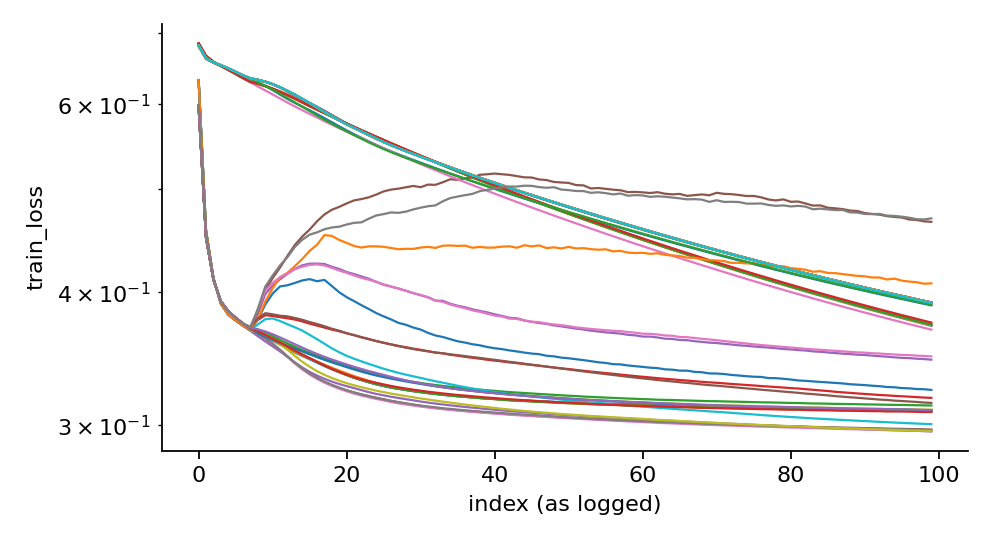
\includegraphics[width=\textwidth]{curve_train_loss.png}
\caption{\texttt{train\_loss}, the mean over seeds per cell.}
\label{fig:curve-1}
\end{figure}
\begin{figure}[tbp]
\centering
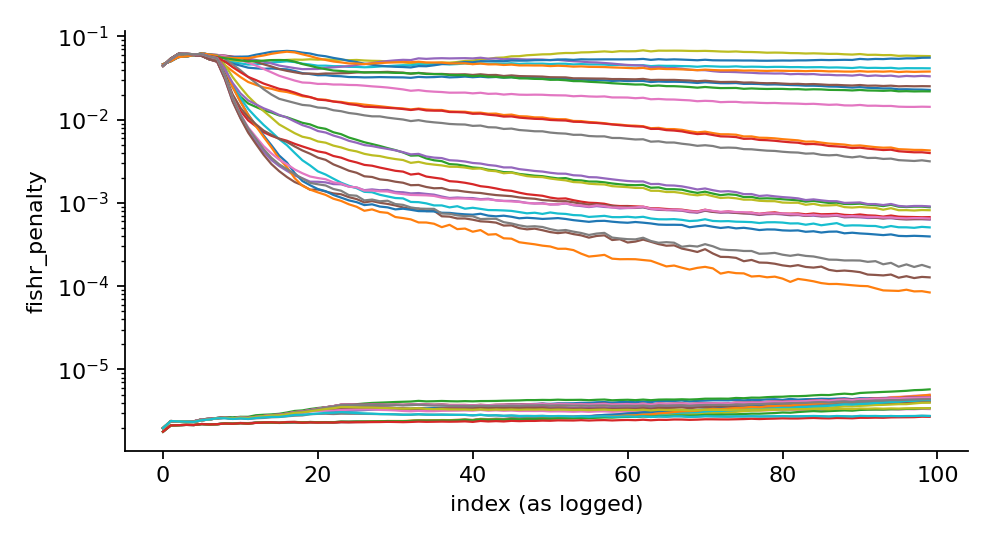
\includegraphics[width=\textwidth]{curve_fishr_penalty.png}
\caption{\texttt{fishr\_penalty}, the mean over seeds per cell.}
\label{fig:curve-2}
\end{figure}
\begin{figure}[tbp]
\centering
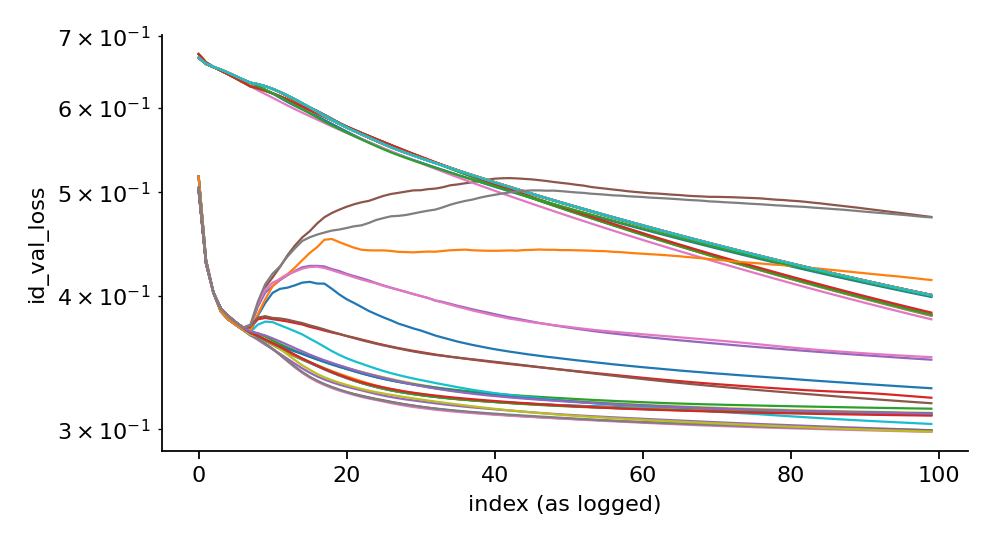
\includegraphics[width=\textwidth]{curve_id_val_loss.png}
\caption{\texttt{id\_val\_loss}, the mean over seeds per cell.}
\label{fig:curve-3}
\end{figure}

\section{Configuration}
The base configuration every run shares (frozen hash \texttt{037f987733ac}); factor levels are in \autoref{tab:summary-ood_len_f1}.
{\footnotesize
\begin{verbatim}
task:
  name: SubsetSumDecisionDataset
  value_range:
  - -5
  - 5
  target_range:
  - 1
  - 10
  weight_range: null
  adversarial_range:
  - 10
  - 30
  noise_prob: 0.0
data:
  train_lengths:
  - 4
  - 5
  - 6
  - 7
  - 8
  ood_lengths:
  - 12
  - 16
  - 64
  ood_value_range:
  - -20
  - 20
  ood_noise_range:
  - 10
  - 30
  ood_noise_prob: 0.5
  n_per_length: 20000
  n_eval_per_length: 2000
  curve_eval_limit: 256
model:
  d_model: 64
  n_heads: 2
  num_layers: 1
  dropout: 0.0
  tropical_impl: legacy
optim:
  lr: 0.0001
  epochs: 100
  batch_size: 100
  eval_batch_size: 256
fishr:
  ema: 0.95
  anneal_iters: 1500
  reset_optimizer: true
\end{verbatim}
}
Store: \texttt{campaigns/tropical/SubsetSumDecision/results}.
\end{document}